% =============================================================================
%
% This is the LaTeX source code of the lecture notes.
%
%
% Author:   Blazej Bucha
% Year:     2022
% Contact:  blazej.bucha@stuba.sk
% Encoding: UTF-8
%
% =============================================================================






% LaTeX Packages
% =============================================================================

\documentclass[a4paper,12pt]{book}
\usepackage[backend=biber,style=iso-authoryear,maxcitenames=2]{biblatex}
\usepackage[main=slovak]{babel}
\usepackage[utf8]{inputenc}
\usepackage[T1]{fontenc}
\usepackage{amsmath}
\usepackage{mathtools}
\usepackage{upgreek}
\usepackage{listings}
\usepackage{xcolor}
\usepackage{graphicx}
\usepackage{accsupp}
\usepackage{csquotes}
\usepackage{cancel}
\usepackage[width=0.95\textwidth,font=small]{caption}
\usepackage[unicode,
            pdfborder={0 0 0},
            colorlinks=true,
            urlcolor=blue,
            citecolor=blue,
            linkcolor=blue]{hyperref}
\usepackage[top=2.5cm, bottom=2.5cm, left=2.5cm, right=2.5cm]{geometry}
\linespread{1.2}
\let\MakeUppercase\relax

% =============================================================================






% Set up the "biblatex" package (see 
% "https://github.com/michal-h21/biblatex-iso690" for further detail)
% =============================================================================

% Add the bibtext file with the references
\addbibresource{references.bib}


% Replace "et al." by the Slovak "a kol."
\DefineBibliographyStrings{slovak}{ andothers = {a\addspace kol\adddot} }


% Change the default separators between the authors of the same bibtex entry.  
% In the main text, we want "a" between two authors.  In the "References" 
% section, we want ";" between all authors.
\DeclareDelimFormat{multinamedelim}{\addspace a \addspace}
\DeclareDelimFormat[bib]{multinamedelim}{\addsemicolon\space}
\DeclareDelimAlias[bib]{finalnamedelim}{multinamedelim}

% =============================================================================






% Define and set the style of code listings
% =============================================================================

% Define custom colours
\definecolor{comments}{rgb}{0.65, 0.65, 0.65}
\definecolor{strings}{rgb}{0.0, 0.3, 0.7}
\definecolor{linenumbers}{rgb}{0.5, 0.5, 0.5}
\definecolor{keywords}{rgb}{0.85, 0.0, 0.0}
\definecolor{backcolour}{rgb}{0.98, 0.98, 0.98}


% Define custom listing style
\lstdefinestyle{codestyle}
{
    backgroundcolor=\color{backcolour},
    commentstyle=\color{comments},
    keywordstyle=\color{keywords},
    numberstyle=\tiny\noncopynumber,
    columns=flexible,
    stringstyle=\color{strings},
    basicstyle=\ttfamily\footnotesize,
    breakatwhitespace=false,
    breaklines=true,
    captionpos=b,
    keepspaces=true,
    numbers=left,
    numbersep=5pt,
    showspaces=false,
    showstringspaces=false,
    showtabs=false,
    tabsize=2
}


% Defines a new command that ensures we can copy the source code from the
% compiled PDF without copying the line numbers
\newcommand{\noncopynumber}[1]
{
    \BeginAccSupp{method=escape,ActualText={}}
    #1
    \EndAccSupp{}
}


% Apply the custom listing style
\lstset{style=codestyle}


% It seems the "listings" package is not able to encode the nice special Slovak
% characters such as "á", "ľ", etc.  Next follows a brute force solution.
\lstset{
  literate={á}{{\'a}}1
           {ä}{{\" a}}1
           {č}{{\v c}}1
           {ď}{{d\kern-0.07cm\char39\kern-0.07cm}}1
           {é}{{\'e}}1
           {í}{{\'i}}1
           {ĺ}{{\'l}}1
           {ľ}{{l\kern-0.12cm\char39\kern-0.05cm}}1
           {ň}{{\v n}}1
           {ó}{{\'o}}1
           {ô}{{\^o}}1
           {ŕ}{{\'r}}1
           {š}{{\v s}}1
           {ť}{{t\kern-0.10cm\char39\kern-0.05cm}}1
           {ú}{{\'u}}1
           {ý}{{\'y}}1
           {ž}{{\v z}}1
           {Á}{{\'A}}1
           {Ä}{{\" A}}1
           {Č}{{\v C}}1
           {Ď}{{\v D}}1
           {É}{{\'E}}1
           {Í}{{\'I}}1
           {Ĺ}{{\'L}}1
           {Ľ}{{L\kern-0.12cm\char39\kern-0.00cm}}1
           {Ň}{{\v N}}1
           {Ó}{{\'O}}1
           {Ô}{{\^O}}1
           {Ŕ}{{\'R}}1
           {Š}{{\v S}}1
           {Ť}{{\v T}}1
           {Ú}{{\'U}}1
           {Ý}{{\'Y}}1
           {Ž}{{\v Z}}1
}


% Add the "as" keyword to the Python listings
\lstdefinelanguage{mypython}[]{Python}{morekeywords={as,True,False}}


% Caption title for listings
\renewcommand\lstlistingname{Zdrojový kód}

% =============================================================================






% Custom commands
% =============================================================================
\newcommand{\diff}{\mathrm d}
\newcommand{\grad}{\mathrm{grad}}
\newcommand{\gidx}{\mathrm g}
\newcommand{\cidx}{\mathrm c}
\let\vec\mathbf

% Let's change the "Dodatok" label of chapters after Conclusions to "Príloha"
\addto\captionsslovak{\renewcommand\appendixname{Príloha}}

% =============================================================================






% Custom hyphenation for some English words in a Slovak text
% =============================================================================

% Isn't there a more clever way to achieve the same?
\hyphenation{New-ton}
\hyphenation{New-to-nov}
\hyphenation{New-to-nom}
\hyphenation{New-to-nov-ho}
\hyphenation{New-to-no-vým}

% =============================================================================






% =============================================================================

\sloppy
\begin{document}

% -----------------------------------------------------------------------------

\chapter*{Predslov}

Mnohé geodetické merania a~úkony využívajú pôsobenie tiažového poľa alebo sú 
ním ovplyvnené, od použitia olovnice až po merania založené na globálnych 
navigačných družicových systémoch.  Táto práca sa zaoberá tiažovým poľom 
s~dôrazom na geodetický kontext.  Určená je predovšetkým ako doplňujúci učebný 
text k~predmetom \emph{Fyzikálna geodézia~1} a~\emph{Fyzikálna geodézia~2} pre 
študentov odboru Geodézia a~kartografia Stavebnej fakulty Slovenskej technickej 
univerzity v~Bratislave.  Niektoré časti by azda mohli byť užitočné aj 
pre~študentov príbuzných vedných odborov alebo jednoducho pre záujemcov 
o~problematiku gravitačného a~tiažového poľa.

Popísané sú základné princípy gravitačného a~tiažového poľa vychádzajúce
z~Newtonovho gravitačného zákona
(Kapitola~\ref{sec:gravitational_and_gravity_field}), sférické harmonické
funkcie (Kapitola~\ref{sec:spherical_harmonic_expansion}), normálne a~poruchové
pole Zeme (Kapitoly~\ref{sec:normal_gravity_field}
a~\ref{sec:disturbing_field}) a~základy určovania geoidu
(Kapitola~\ref{sec:geoid_determination}).  Zvolili sme formu, ktorú na základe
desaťročných skúseností s~výučbou fyzikálnej geodézie považujeme za
najvhodnejšiu pre očakávaných čitateľov, študentov geodézie a~kartografie.
Znamená to, že hoci intelektuálne potešenie zo spoznávania tiažového poľa je
bezodné, predsa len si vyžaduje pokročilé matematické zručnosti a~nepochybne
aj~isté zanietenie.  Snažili sme sa preto o~výklad, ktorý by bol jednoduchý,
zrozumiteľný, úplný, nápomocný a~súčasne i~podnecujúci.  Na miestach, kde sme
to považovali za vhodné, text sme doplnili o~počítačový kód, ktorý prakticky
demonštruje diskutovanú problematiku.  Nádejame sa, že jeho štúdiom,
testovaním a~úpravou je možné niektorým konceptom porozumieť jednoduchšie.

Aj keď napísaniu tejto práce bolo venované veľké úsilie, bolo by prekvapivé, ak 
by sa v~nej nenašli časti, ktoré mohli byť spracované zrozumiteľnejšie, či 
témy, ktoré v~nej obsiahnuté nie sú, no mohli či mali byť diskutované.  Skôr 
než za uzavretý študijný podklad považujeme tento učebný text za živý postupne 
sa zdokonaľujúci materiál.  Všetky zdrojové kódy sú preto voľne prístupné 
a~pripomienkovateľné na adrese 
\url{https://github.com/blazej-bucha/physical-geodesy-lecture-notes}.

Práca bola napísaná v~textovom editore Vim~v8.2 použitím typografického systému
\TeX.  Skompilovaná bola programom \texttt{pdfTex}~v3.14159265-2.6-1.40.21.
Mapy boli pripravené v~\texttt{GMT}~v6.1.1.  Obrázky boli zhotovené v~programe
\texttt{Inkscape}~v1.0.2.  Väčšina výpočtového kódu je napísaná
a~otestovaná v~jazyku \texttt{Python}~v3.9.2 s~využitím modulov
\texttt{NumPy}~v1.20.3, \texttt{Matplotlib}~v3.5.0 a~\texttt{SciPy}~v1.7.3.
Časť výpočtového kódu je napísaná v~jazyku~C a~v~prostredí~MATLAB~R2021b.
S~týmito aplikáciami sme interagovali pod operačným systémom Debian GNU/Linux
11 (Bullseye).  S~výnimkou programu MATLAB ide o~slobodný voľne šíriteľný
software.  Vyslovujeme preto vďaku a~slová ocenenia veľkej komunite
excelentných programátorov za to, že poskytujú slobodný prvotriedny software.

Úprimné slová vďaky patria v~neposlednom rade všetkým, ktorí akýmkoľvek
spôsobom prispeli k~tejto práci. \emph{Na záver tu budeš doplnený/á, ak s~tým
budeš súhlasiť!}


\vspace{4ex}

\noindent V~Bratislave XX.~XX.~2022 \hfill Blažej Bucha






% -----------------------------------------------------------------------------
\tableofcontents
\newpage
% -----------------------------------------------------------------------------






% -----------------------------------------------------------------------------

\chapter*{Úvod}
\label{sec:introduction}

Tvar Zeme možno definovať niekoľkými spôsobmi v~závislosti od kontextu 
\parencite{MoritzTheFigureOfTheEarth}.  Azda najprirodzenejšie je definovať 
tvar Zeme jej skutočným fyzickým povrchom, ktorý je viditeľný voľným okom.  
Tento povrch obsahuje nespočetné množstvo zložitých terénnych útvarov, 
napríklad strmé útesy či rokliny.  Hoci sú takéto oblasti krásne na pohľad, 
znemožňujú aplikáciu istej časti potrebného matematického aparátu, okrem iného 
plošnú integráciu.  Skúmať takto chápaný zemský povrch je preto možné iba po 
istom vyhladení.  Napriek vyhladeniu však ide stále o~veľmi zložitú plochu.

K~definovaniu tvaru Zeme môžeme pristúpiť aj~iným spôsobom.  Približne dve
tretiny zemského povrchu tvorí voda v~podobe oceánov a~morí.  Voda má za istých
okolností tú vlastnosť, že existuje fyzikálna veličina, ktorá je na jej povrchu
konštantná.  Táto vlastnosť by teda mohla umožniť akúsi predikciu morskej
hladiny i popod, resp. ponad kontinenty.  Získali by sme tak geometricky
jednoduchšiu a~hladkejšiu plochu ako v~predošlom prístupe, navyše aj
s~istými relatívne jednoducho uchopiteľnými fyzikálnymi vlastnosťami.  Takáto
definícia tvaru Zeme bola navrhnutá C.~F.~Gaussom (1777--1855) a~podľa návrhu
J.~B.~Listinga (1808--1882) nazývame túto plochu \emph{geoid}.  Veličina, ktorá
je konštantná na povrchu geoidu sa nazýva \emph{tiažový potenciál}.

\emph{Fyzikálna geodézia} je vedná disciplína zaoberajúca sa určovaním tvaru
Zeme, jej tiažovým poľom a~ich zmenami v~čase.  Študované sú oba vyššie opísané
prístupy k~tvaru Zeme, pričom historicky bol predmetom záujmu ako prvý geoid.
Hoci prirodzená, no matematicky odvážna myšlienka určovať priamo fyzický povrch
Zeme pochádza už od E.~H.~Brunsa (1848--1919), do popredia záujmu ju dostal až
v~polovici 20. storočia M.~S.~Molodenskij (1909--1991).  Aj~v~tomto prípade je
však tvar Zeme určovaný z~informácie o~tiažovom poli.  Napĺňať jednu zo 
základných úloh geodéziu, štúdium tvaru Zeme, teda znamená študovať aj tiažové
pole Zeme.






% -----------------------------------------------------------------------------

\chapter{Gravitačné a~tiažové pole}
\label{sec:gravitational_and_gravity_field}






\section{Newtonov gravitačný zákon}
\label{sec:newton_law}

Dva hmotné body $P$ a~$Q$ sa navzájom priťahujú \emph{gravitačnou silou}
%
\begin{equation}
\label{eq:newton_law}
\vec F_\gidx = -G \frac{m_P \, m_Q}{l^2} \, \frac{\vec r}{l}{.}
\end{equation}
%
Symbol $G$ označuje gravitačnú konštantu, $m_P$ a~$m_Q$ predstavujú hmotnosti 
hmotných bodov, $\vec r$ je vektor definovaný polohou bodov $P$ a~$Q$ so 
začiatkom v~bode $Q$ a~$l$ je vzdialenosť medzi hmotnými bodmi, $l = \| \vec 
r \|$.  Záporné znamienko v~rovnici znamená, že vektor sily má začiatok v~bode 
$P$ a~smeruje do bodu $Q$ (Obrázok~\ref{fig:newton_law}).

\begin{figure}[b]
\centering
\input{./fig-newton-law.pdf_tex}
%\captionsetup{width=0.8\textwidth}
\caption{Gravitačná sila $\vec F_\gidx$, ktorou pôsobí hmotný bod $Q$ na hmotný 
bod $P$.  Vektor $\vec F_\gidx$ je z~dôvodov vizualizácie mierne odsadený od 
spojnice bodov $P$ a~$Q$.}
\label{fig:newton_law}
\end{figure}

Rovnica~(\ref{eq:newton_law}) predstavuje \emph{gravitačný zákon} publikovaný
I.~Newtonom (1642--1727) v~práci \emph{Philosophi\ae Naturalis Principia
Mathematica} z~roku 1687.  Hovorí, že každý hmotný bod vo vesmíre priťahuje
každý iný hmotný bod silou, ktorej veľkosť je priamo úmerná súčinu ich 
hmotností a~nepriamo úmerná štvorcu ich vzdialenosti.  Smer sily je daný 
spojnicou hmotných bodov \parencite{Kellogg1967}.  \emph{Hmotný bod} je 
idealizovaný pojem predstavujúci časticu s~nulovým rozmerom a~konečnou 
nenulovou hmotnosťou bez akýchkoľvek ďalších vlastností či štruktúry.  Hodnota 
gravitačnej konštanty odporúčaná od roku 2018 \emph{Komisiou pre dáta vo vede 
a~technológiách} (CODATA) je $G = (6.67430 \pm 0.00015) \times 10^{-11} 
\ \mathrm{m}^3 \ \mathrm{kg}^{-1} \ \mathrm{s}^{-2}$.

Nech planéta obieha okolo Slnka (Obrázok~\ref{fig:orbital_motion}).  Označme 
polohu planéty v~čase $t_0$ symbolom $P(t_0)$ a~vektor jej okamžitej rýchlosti 
symbolom $\vec v(t_0)$.  Predpokladajme, že planéta má v~čase $t_0$ udelenú 
nenulovú rýchlosť, teda $\| \vec v(t_0) \| > 0$.  Ak by od času $t_0$ 
nepôsobila na planétu žiadna sila, \emph{Newtonov pohybový zákon} hovorí, že 
planéta by sa ďalej pohybovala rovnomerným priamočiarym pohybom v~smere vektora 
$\vec v(t_0)$.  Za istý čas by sa teda dostala do bodu $P'(t_1)$.  Jediný 
spôsob ako zmeniť túto dráhu je pôsobiť na planétu silou.  
Z~rovnice~(\ref{eq:newton_law}) vyplýva, že v~čase $t_0$ pôsobí na planétu 
gravitačnou silou $\vec F_\gidx(t_0)$ Slnko, pričom smer sily je daný spojnicou 
planéty a~Slnka.  Gravitačná sila preto pritiahne planétu v~smere vektora $\vec 
F_\gidx(t_0)$, čím zmení hypotetickú trajektóriu, ktorou by sa planéta 
pohybovala bez pôsobenia tejto sily.  V~kombinácii s~vektorom rýchlosti 
gravitačná sila spôsobí, že planéta sa dostane do bodu $P(t_1)$.  V~čase $t_1$ 
sa opísaná situácia opakuje, pričom vektory rýchlosti a~sily už majú iný smer 
a~s~vysokou pravdepodobnosťou aj inú veľkosť.  Gravitačná sila Slnka teda 
zakrivuje trajektóriu planéty \emph{v každom okamihu}.

\begin{figure}
\centering
\input{./fig-orbital-motion-ideal.pdf_tex}
\caption{Obeh planéty okolo Slnka}
\label{fig:orbital_motion}
\end{figure}

Podobným spôsobom je možné vysvetliť pomocou Newtonovho gravitačného zákona 
mnoho ďalších prírodných javov, napríklad príliv a~odliv, či zodpovedať otázku, 
prečo majú planéty približne sférický tvar.  Je pozoruhodné, že hoci 
rovnica~(\ref{eq:newton_law}) bola odpozorovaná z~pohybu nebeských telies, 
zhoduje sa i~s experimentmi, ktoré boli vykonané na vzdialenosť niekoľkých 
desiatok mikrometrov \parencite{Lee2020}.  Napriek uvedenému, azda je potrebné 
spomenúť aj~skutočnosť, že Newtonov gravitačný zákon je \emph{nesprávny} 
\parencite{Feynman}.  Predpokladá napríklad, že zmena hmotnosti či vzdialenosti 
má okamžitý gravitačný účinok, teda aj~v~prípade telies nachádzajúcich sa vo 
veľkých vzdialenostiach.  Tento predpoklad je však v~rozpore s~experimentálne 
potvrdenou Einsteinovou špeciálnou teóriou relativity.  Tá hovorí, že žiadny 
signál, a~teda ani ten gravitačný, sa nemôže šíriť rýchlosťou väčšou ako je 
rýchlosť svetla.  Pre účely fyzikálnej geodézie sú však chyby spôsobené 
nepresnosťami Newtonovho gravitačného zákona väčšinou zanedbateľné.  Táto 
teória tak aj dnes, viac ako tristo rokov po jej vzniku, tvorí chrbtovú kosť 
fyzikálnej geodézie.






\subsection{Gravitačné zrýchlenie}
\label{sec:gg}

Gravitačná sila~(\ref{eq:newton_law}) pôsobiaca medzi hmotnými bodmi~$P$ 
a~$Q$~závisí od hmotnosti oboch hmotných bodov.  Skúsme preto normovať vektor 
gravitačnej sily hmotnosťou $m_P$.  Získame tým vektorovú veličinu, ktorá sa 
nazýva \emph{gravitačné zrýchlenie},
%
\begin{equation}
\label{eq:gg_point_mass}
\vec g_\gidx(P) = \frac{\vec F_\gidx}{m_P} = -G \frac{m}{l^2} \, \frac{\vec
r}{l}{,}
\end{equation}
%
kde $m = m_Q$.  Rovnica~(\ref{eq:gg_point_mass}) hovorí, že hmotný
bod~$Q$ udeľuje hmotnému bodu $P$ zrýchlenie $\vec g_\gidx(P)$.   Inými
slovami, gravitačné zrýchlenie $\vec g_\gidx(P)$ nezávisí od hmotnosti hmotného
bodu $P$, začiatok má v~bode $P$ a~smeruje do hmotného bodu $Q$.  V~súvislosti
s~hmotným bodom $P$ je preto možné pre jednoduchosť vynechať prívlastok
\emph{hmotný} a~považovať $P$ za geometrický bod bez fyzikálnych vlastností.
Skutočnosť, že gravitačné zrýchlenie priťahovaného telesa nezávisí od jeho
hmotnosti experimentálne potvrdil Gaileo Gailei (1564--1642).

Z~predchádzajúcej kapitoly vyplýva, že v~sústave $N$ hmotných bodov je celkové 
gravitačné zrýchlenie dané vektorovým súčtom čiastkových
gravitačných zrýchlení, ktoré sú udeľované jednotlivými hmotnými bodmi
(Obrázok~\ref{fig:gg_n_point_masses}),
%
\begin{equation}
\label{eq:gg_N_point_masses}
\vec g_\gidx(P) = \sum_{i = 1}^{N}\vec g_{\gidx,i}(P) = -G \sum_{i = 1}^{N}
\frac{m_i}{l_i^2} \, \frac{\vec r_i}{l_i}{.}
\end{equation}

\begin{figure}[b]
\centering
\input{./fig-gg-n-point-masses.pdf_tex}
\caption{Vektory gravitačného zrýchlenia v~bode $P$ generované sústavou piatich
hmotných bodov}
\label{fig:gg_n_point_masses}
\end{figure}

Newtonov gravitačný zákon~(\ref{eq:newton_law}) 
a~rovnice~(\ref{eq:gg_point_mass}) a~(\ref{eq:gg_N_point_masses}) platia iba 
pre hmotné body.  Tento tvar rovníc je možné aplikovať napríklad na popis 
pohybu planét Slnečnej sústavy.  Rozmery planét sú totiž natoľko zanedbateľné 
v~porovnaní s~ich vzájomnou vzdialenosťou, že sa nedopustíme nerozumne veľkej 
chyby, ak hmotnosti týchto telies sústredíme do ich ťažísk a~zanedbáme ich 
tvar.  Menej priaznivá situácia nastáva vtedy, keď sa bod $P$ nachádza 
v~blízkosti priťahujúceho telesa, ktoré má komplikovaný tvar a~hustotu.  
Príkladom je družica na nízkej obežnej dráhe Zeme.  V~súlade s~predchádzajúcim 
odsekom by sme preto mohli nahradiť Zem množinou hmotných bodov, či už 
s~konečným alebo nekonečným počtom, a~výsledné gravitačné zrýchlenie pôsobiace 
na družicu získať vzťahom~(\ref{eq:gg_N_point_masses}).  Označenie takéhoto 
riešenia za nesprávne však nebude prekvapivé, keď si spomenieme, že hmotný bod 
bol definovaný ako bezrozmerný (Kapitola~\ref{sec:newton_law}).  Bezrozmernými 
hmotnými bodmi nemožno aproximovať objem telesa.

Zaveďme preto pojem \emph{všeobecné teleso}, ktoré má konečný objem $\tau$ 
a~jeho hustota $\rho$ je daná ohraničenou funkciou polohy 
(Obrázok~\ref{fig:gravitating_body}).  Rozdeľme toto teleso na nekonečne veľa 
diferenciálnych hmotných elementov $\diff m = \rho \, \diff \tau$.  Hustota 
$\rho$ sa môže meniť medzi hmotnými elementmi $\diff m$ v~závislosti od 
štruktúry daného telesa, ale nesmie sa meniť v~rámci elementu samotného.  Aby 
sme mohli aplikovať Newtonov gravitačný zákon, ktorý je formulovaný pre hmotné 
body, budeme musieť predpokladať, že diferenciálne hmotné elementy $\diff m$, 
akokoľvek sú malé, nikdy nie sú identické s~hmotnými bodmi, a hmota týchto 
elementov je koncentrovaná do jedného bodu \parencite{Kellogg1967}.

\begin{figure}
\centering
\input{./fig-gravitating-body.pdf_tex}
\caption{Všeobecné teleso}
\label{fig:gravitating_body}
\end{figure}

Po uvážení $\diff m = \rho \, \diff \tau$ bude gravitačné zrýchlenie generované
hmotným elementom $\diff m$ dané vzťahom
%
\begin{equation}
\label{eq:gg_dm}
\diff \vec g_\gidx(P) = -G \frac{\vec r}{l^3} \rho \, \diff\tau{,}
\end{equation}
%
kde vektor $\vec r$ je definovaný rozdielom polohových vektorov bodov $P$
a~$Q$,
%
\begin{equation}
\label{eq:r}
\vec r =
%
\begin{bmatrix}
x - x_Q \\
y - y_Q \\
z - z_Q
\end{bmatrix}
{,}
\end{equation}
%
a~$l = \| \vec r \|$ je jeho veľkosť, teda Euklidovská vzdialenosť medzi bodmi
$P$ a~$Q$,
%
\begin{equation}
\label{eq:l}
l = \sqrt{(x - x_Q)^2 + (y - y_Q)^2 + (z - z_Q)^2}{.}
\end{equation}
%
Celkové gravitačné zrýchlenie generované všeobecným telesom získame teda
integráciou vzťahu~(\ref{eq:gg_dm}),
%
\begin{equation}
\label{eq:gg_body}
\vec g_\gidx(P) = -G \iiint\limits_{\tau} \frac{\vec r}{l^3} \, \rho \, 
\diff\tau{.}
\end{equation}
%
Tento vzťah už môže byť korektne použitý na výpočet gravitačného zrýchlenia 
všeobecného telesa (napríklad Zeme) v~ľubovoľnom bode~$P$ (napríklad v~ťažisku 
družice).

Vektor gravitačného zrýchlenia veľmi úzko súvisí s~veličinou, ktorú je možné
odmerať na povrchu Zeme, a~tak má pre fyzikálnu geodéziu kľúčový význam.
V~sústave jednotiek SI má gravitačné zrýchlenie jednotku $\mathrm{m}\
\mathrm{s}^{-2}$.  Veľmi často je možné stretnúť sa aj s~jednotkou $1\
\mathrm{Gal} = 10^{-2}\ \mathrm{m}\ \mathrm{s}^{-2}$ pomenovanou podľa Galilea
Galileiho, prípadne s~jej násobkami $1\ \mathrm{mGal} = 10^{-5}\ \mathrm{m}\
\mathrm{s}^{-2}$ a~$1\ \upmu \mathrm{Gal} = 10^{-8}\ \mathrm{m}\
\mathrm{s}^{-2}$.

Obrázok~\ref{fig:gg_grav_sr_2arcsec} zobrazuje priebeh veľkosti vektora
gravitačného zrýchlenia v~oblasti Vysokých a~Nízkych Tatier.  Z~porovnania
s~topografiou (Obrázok~\ref{fig:h_grav_sr_2arcsec}) je zrejmé, že gravitačné
zrýchlenie je veľmi závislé od lokálnych hmôt, teda od hustoty a~tvaru blízkych
diferenciálnych elementov $\diff m = \rho \, \diff \tau$ a~ich vzdialenosti $l$
od bodu $P$, v~ktorom je gravitačné zrýchlenie skúmané (pozri
vzťah~\ref{eq:gg_body}).  Na lokálnej úrovni je možné pozorovať, že v~miestach
s~veľkou nadmorskou výškou je veľkosť gravitačného zrýchlenia spravidla menšia
ako v~miestach s~malou nadmorskou výškou a~naopak.  Z~globálneho hľadiska je
tiažové zrýchlenie ovplyvnené najmä tvarom Zeme, predovšetkým jej sploštením,
a~rozsiahlymi hustotnými celkami vo vnútri Zeme.

\begin{figure}
\centering
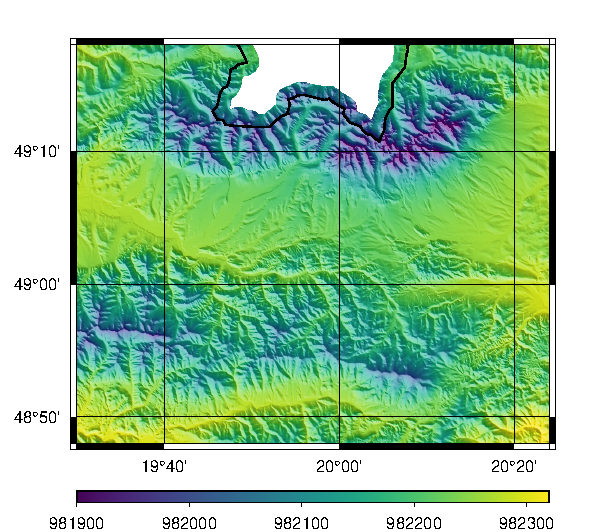
\includegraphics{./fig-gg-grav-sr-2arcsec.pdf}
\caption{Veľkosť vektora gravitačného zrýchlenia $\| \vec g_\gidx \|$ na 
zemskom povrchu v~oblasti Vysokých a~Nízkych Tatier (jednotky mGal).  Dáta sú 
prevzaté z~modelu \texttt{grav-sr-2arcsec} \parencite{GravSR2arcsec}.}
\label{fig:gg_grav_sr_2arcsec}
\end{figure}

\begin{figure}
\centering
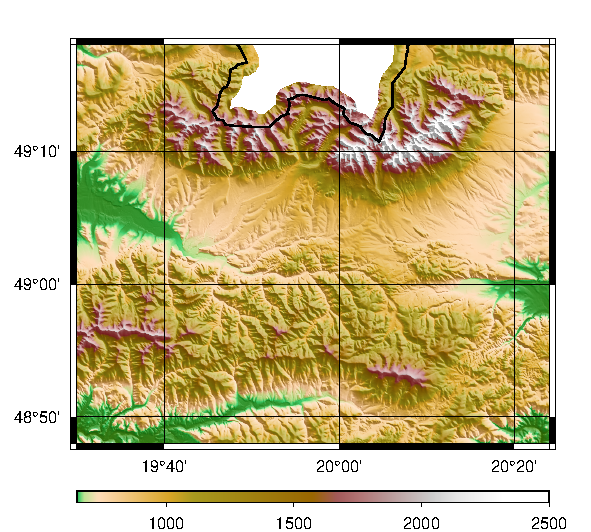
\includegraphics{./fig-h-grav-sr-2arcsec.pdf}
\caption{Topografia v~oblasti Vysokých a~Nízkych Tatier vyjadrená pomocou 
elipsoidickej výšky (jednotky~m).  Dáta sú prevzaté z~modelu 
\texttt{grav-sr-2arcsec} \parencite{GravSR2arcsec}.}
\label{fig:h_grav_sr_2arcsec}
\end{figure}







\subsection{Gravitačný potenciál}
\label{sec:vg}

Gravitačné zrýchlenie $\vec g_\gidx$ je vektorová veličina, ktorá má v~každom 
bode definovanú trojicu reálnych čísel.  V~niektorých situáciách je výhodnejšie 
pracovať so skalárnou veličinou, teda takou, ktorá má v~bode~$P$ definované 
práve jedno reálne číslo.  Tento prístup je mladší ako Newtonov gravitačný 
zákon zhruba o~jedno storočie \parencite{MacMillan1930,Jekeli2015}.  Fenomén 
gravitácie chápe ako \emph{pole}, ktorého vlastnosti môžu byť popísané rôznymi 
vzájomne súvisiacimi veličinami, pričom však ide stále o~to isté pole.  
S~konceptom potenciálu poľa prišiel podľa \textcite{MacMillan1930} taliansky 
matematik a~astronóm J.~L.~Lagrange (1736--1813).  Ak by sme teda našli 
skalárnu veličinu gravitačného poľa, informáciu poskytnutú troma číslami 
v~podobe gravitačného vektora by sme dokázali zredukovať na jedno jediné číslo 
bez straty informácie o~poli samotnom.  Skalárna veličina gravitačného poľa sa 
nazýva \emph{gravitačný potenciál} a~označuje sa symbolom $V_\gidx$.

Gravitačný potenciál definujeme pomocou gravitačného zrýchlenia.  Pre lepšie
pochopenie vzťahu medzi gravitačným zrýchlením a~gravitačným potenciálom však
najprv predstavíme diferenciálny operátor gradient a~až následne pristúpime
k~samotnej definícii gravitačného potenciálu.

V~trojrozmernom pravouhlom súradnicovom systéme $x$, $y$, $z$ je operátor
gradient definovaný nasledovne,
%
\begin{equation}
\label{eq:gradient}
\nabla = \grad = \vec e_1 \frac{\partial}{\partial x} + \vec e_2
\frac{\partial}{\partial y} + \vec e_3 \frac{\partial}{\partial z} =
\begin{bmatrix}
\dfrac{\partial}{\partial x} \\[2ex]
\dfrac{\partial}{\partial y} \\[2ex]
\dfrac{\partial}{\partial z}
\end{bmatrix}
{,}
\end{equation}
%
kde $\vec e_1$, $\vec e_2$ a~$\vec e_3$ predstavujú jednotkové vektory
rovnobežné so smerom súradnicových osí (Obrázok~\ref{fig:3d_coord_system}),
%
\begin{equation}
\label{eq:unit_vectors}
\vec e_1 =
\begin{bmatrix}
1\\
0\\
0\\
\end{bmatrix}
{,} \quad
%
\vec e_2 =
\begin{bmatrix}
0\\
1\\
0
\end{bmatrix}
%
{,}\quad
%
\vec e_3 =
\begin{bmatrix}
0\\
0\\
1
\end{bmatrix}
{,}
\end{equation}
%
pričom
%
\begin{equation}
\label{eq:unit_vectors_unit_length}
\| \vec e_i \| = 1{,} \quad i = 1, 2,3{.}
\end{equation}
%
Aplikáciou operátora gradient na \emph{skalárnu} funkciu $f(x, y, z)$ získame 
\emph{vektorovú} funkciu,
%
\begin{equation}
\begin{split}
\vec f(x, y, z) &= \nabla f(x, y, z) = \grad \ f(x, y, z)\\
%
&= \vec e_1 \frac{\partial f(x, y, z)}{\partial x} + \vec e_2 \frac{\partial
f(x, y, z)}{\partial y} + \vec e_3 \frac{\partial f(x, y, z)}{\partial z} =
\begin{bmatrix}
\dfrac{\partial f(x, y, z)}{\partial x} \\[2ex]
\dfrac{\partial f(x, y, z)}{\partial y} \\[2ex]
\dfrac{\partial f(x, y, z)}{\partial z}
\end{bmatrix}
{.}
\end{split}
\end{equation}
%
Vektorová funkcia $\vec f(x, y, z)$ \emph{udáva smer a~veľkosť najväčšieho
nárastu} funkcie $f(x, y, z)$ v~bode so súradnicami $x$, $y$ a~$z$.  Jednotlivé 
zložky vektorovej funkcie $\vec f(x, y, z)$, teda parciálne derivácie $\partial 
f \slash \partial x$, $\partial f \slash \partial y$ a $\partial f \slash 
\partial z$, udávajú zmenu skalárnej funkcie $f(x, y, z)$ v~smere jednotkových 
vektorov $\vec e_1$, $\vec e_2$ a $\vec e_3$ v~bode, v~ktorom sú derivácie 
vypočítané.  Operátor gradient  je \emph{lineárny}, teda pre diferencovateľné 
funkcie $f$ a~$g$ a~konštantu $c$ platí
%
\begin{equation}
\label{eq:gradient_additivity}
\nabla \left(f + g \right) = \nabla f + \nabla g
\end{equation}
%
a
%
\begin{equation}
\label{eq:gradient_homogenity}
\nabla (c \, f) = c \, \nabla f{.}
\end{equation}
%
Numerická ukážka aplikácie operátora gradient je uvedená 
v~Prílohe~\ref{app:numerical_application_of_gradient}.

\begin{figure}
\centering
\input{./fig-3d-coord-system.pdf_tex}
\caption{Trojrozmerný pravouhlý súradnicový systém a jednotkové vektory}
\label{fig:3d_coord_system}
\end{figure}

Gravitačný potenciál môžeme definovať pomocou operátora gradient nasledovne.  
Gravitačný potenciál je skalárna funkcia, ktorá vyhovuje rovnici 
\parencite{SansoGeoidDetermination}
%
\begin{equation}
\label{eq:gg_grad_vg}
\vec g_\gidx(P) = \nabla V_\gidx(P)
\end{equation}
%
a~spĺňa podmienku
%
\begin{equation}
\label{eq:vg_at_infty}
\lim_{P \to \infty} V_\gidx(P) = 0{.}
\end{equation}
%
Vzťah~(\ref{eq:gg_grad_vg}) hovorí, že vektor gravitačného zrýchlenia udáva 
smer a~veľkosť najväčšieho nárastu gravitačného potenciálu.  
Rovnica~(\ref{eq:vg_at_infty}) znamená, že gravitačný potenciál nadobúda 
v~nekonečnej vzdialenosti od telesa nulovú hodnotu.  Tento vzťah zabezpečuje, 
že existuje práve jedna funkcia $V_\gidx$ vyhovujúca 
rovnici~(\ref{eq:gg_grad_vg}) \parencite{SansoGeoidDetermination}.  Keďže 
podmienka (\ref{eq:vg_at_infty}) bola zvolená, \emph{gravitačný potenciál je 
relatívna veličina}.

Gravitačný potenciál hmotného bodu je daný vzťahom
%
\begin{equation}
\label{eq:vg_point_mass}
V_\gidx(P) = \frac{G \, m}{l}{.}
\end{equation}
%
Overme, či tento vzťah vyhovuje rovniciam~(\ref{eq:gg_grad_vg})
a~(\ref{eq:vg_at_infty}).  Aplikujme operátor gradient~(\ref{eq:gradient})
na gravitačný potenciál~(\ref{eq:vg_point_mass}) s~využitím~(\ref{eq:l}),
%
\begin{equation}
\label{eq:gg_from_vg_point_mass}
\nabla V_\gidx(P) = G \, m \, \nabla \left( \frac{1}{l} \right) =
%
G \, m
\begin{bmatrix}
\dfrac{\partial}{\partial x} \left( \dfrac{1}{l} \right)\\[2ex]
\dfrac{\partial}{\partial y} \left( \dfrac{1}{l} \right)\\[2ex]
\dfrac{\partial}{\partial z} \left( \dfrac{1}{l} \right)
\end{bmatrix}
%
=
%
-G \, m
%
\begin{bmatrix}
\dfrac{x - x_Q}{l^3}{,}\\[2ex]
\dfrac{y - y_Q}{l^3}{,}\\[2ex]
\dfrac{z - z_Q}{l^3}
\end{bmatrix}
{.}
\end{equation}
%
Vzťah~(\ref{eq:gg_from_vg_point_mass}) predstavuje gravitačné zrýchlenie $\vec 
g_\gidx(P)$ z~rovnice~(\ref{eq:gg_point_mass}), čím bola dokázaná 
rovnosť~(\ref{eq:gg_grad_vg}).  Platnosť vzťahu~(\ref{eq:vg_at_infty}), teda
%
\begin{equation}
\lim_{l \to \infty} \frac{G \, m}{l} = 0{,}
\end{equation}
%
je zrejmá.

V~sústave $N$ hmotných bodov je celkový gravitačný potenciál daný súčtom
čiastkových príspevkov jednotlivých hmotných bodov,
%
\begin{equation}
\label{eq:vg_N_point_masses}
V_\gidx(P) = \sum_{i = 1}^{N} V_{\gidx,i}(P) = G \sum_{i = 1}^{N}\frac{
m_i}{l_i}{.}
\end{equation}
%
Podobne ako v~rovnici~(\ref{eq:gg_from_vg_point_mass}) je možné
presvedčiť sa, že aplikovaním operátora gradient na gravitačný
potenciál~(\ref{eq:vg_N_point_masses}) získame vektor gravitačného
zrýchlenia~(\ref{eq:gg_N_point_masses}).  Rovnice~(\ref{eq:gg_grad_vg}) 
a~(\ref{eq:vg_at_infty}) teda platia i~v~prípade gravitačného
potenciálu, ktorý je generovaný sústavou $N$ hmotných bodov.

Od gravitačného potenciálu, ktorý je generovaný $N$ hmotnými bodmi prejdeme ku
gravitačnému potenciálu všeobecného telesa podobnou úvahou ako
v~Kapitole~\ref{sec:gg}.  Teleso rozdelíme na diferenciálne hmotné elementy
$\diff m = \rho \, \diff \tau$ a~gravitačný potenciál získame integráciou,
%
\begin{equation}
\label{eq:vg_body}
V_\gidx(P) = G \iiint\limits_{\tau} \frac{\rho}{l} \diff\tau{.}
\end{equation}
%
Dôkaz, že rovnica~(\ref{eq:vg_body}) vyhovuje prijatej definícii gravitačného
potenciálu (\ref{eq:gg_grad_vg} a~\ref{eq:vg_at_infty}) vynecháme, no je
dostupný napríklad v~\textcite{MacMillan1930}.

K~interpretácii gravitačného potenciálu je možné pristúpiť aj z~fyzikálneho 
hľadiska.  Bez podrobného odvodenia sa obmedzíme na tvrdenie, že hodnota 
gravitačného potenciálu v~bode $P$ predstavuje prácu, ktorú musí vykonať 
gravitačné pole pri premiestnení hmotného bodu s~hmotnosťou $1\ \mathrm{kg}$ 
z~miesta s~nulovým potenciálom (v geodézii nekonečno, pozri 
vzťah~\ref{eq:vg_at_infty}) do bodu $P$ 
\parencite{MacMillan1930,Kellogg1967,TorgeGeodesy}.  \emph{Práca} je dráhový 
účinok sily, v~tomto prípade gravitačnej.  Gravitačná sila má tú vlastnosť, že 
práca spôsobená jej silovým účinkom \emph{nezávisí} od dráhy, dôležitý je iba 
začiatočný a~koncový bod dráhy.  Ak sú začiatočný a~koncový bod totožné, práca 
je nulová.  Bez tejto vlastnosti by nebolo možné nájsť skalárnu funkciu 
$V_\gidx$, ktorá by vyhovovala rovnici~(\ref{eq:gg_grad_vg}).

Na rozdiel od vektora gravitačného zrýchlenia, gravitačný potenciál nedokážeme
priamo merať.  Vo fyzikálnej geodézii vystupuje často ako neznáma funkcia,
ktorú sa snažíme určiť, napríklad z~vektora gravitačného zrýchlenia.  V~sústave
SI má gravitačný potenciál fyzikálnu jednotku $\mathrm{m}^2\ \mathrm{s}^{-2}$.
Ukážka priebehu gravitačného potenciálu v~oblasti Vysokých a~Nízkych Tatier je
uvedená na Obrázku~\ref{fig:vg_grav_sr_2arcsec}.

\begin{figure}
\centering
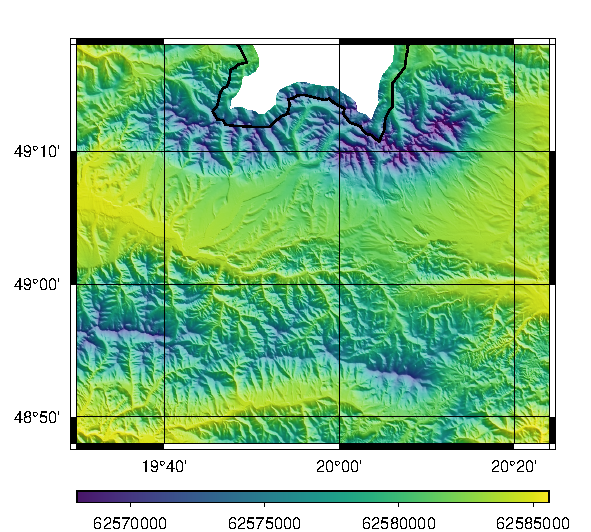
\includegraphics{./fig-vg-grav-sr-2arcsec.pdf}
\caption{Gravitačný potenciál $V_\gidx$ na zemskom povrchu v~oblasti Vysokých
a~Nízkych Tatier (jednotky $\mathrm{m}^2 \ \mathrm{s}^{-2}$).  Dáta sú prevzaté
z~modelu \texttt{grav-sr-2arcsec} \parencite{GravSR2arcsec}.}
\label{fig:vg_grav_sr_2arcsec}
\end{figure}






\section{Teória potenciálu}
\label{sec:potential_theory}

Rovnica~(\ref{eq:vg_body}) sa v~literatúre nazýva \emph{Newtonov
integrál}.  Hovorí, že ak poznáme tvar a~priestorové rozloženie hustoty telesa,
gravitačný potenciál tohto telesa môže byť vypočítaný.  Newtonov
integrál má vo fyzikálnej geodézii kľúčový význam, nakoľko v~gravitačnom
potenciáli je obsiahnutá informácia o~celom gravitačnom poli (pozri
Kapitolu~\ref{sec:newton_law}).

Newtonov integrál položil základy novej oblasti matematiky a~matematickej 
fyziky s~názvom \emph{teória potenciálu}.  Podľa \textcite{MacMillan1930} 
siahajú jej začiatky k~francúzskemu matematikovi, fyzikovi, astronómovi 
a~politikovi P.~S.~Laplaceovi (1749--1827).  Ten si uvedomil, že gravitačný 
potenciál každého všeobecného telesa má spoločné určité vlastnosti, čím vzniká 
zaujímavá množina funkcií hodná podrobnejšieho štúdia.  Významnosť teórie 
potenciálu iba potvrdzuje skutočnosť známa približne od čias C.~F.~Gaussa, 
a~síce že túto teóriu je možné aplikovať nielen na gravitačné pole, ale 
napríklad aj na magnetické, či elektrostatické pole (spomeňme si na Coulombov 
zákon a~porovnajme ho s~Newtonovým gravitačným zákonom~\ref{eq:newton_law}).  
Teória potenciálu teda študuje vzťah~(\ref{eq:vg_body}) vo všeobecnom zmysle, 
zaoberá sa rozličnými zdrojmi poľa (hmotný bod, hmotná priamka, nekonečne tenká 
vrstva, všeobecné teleso a~pod.) s~rôznym priestorovým rozložením hustôt 
(konštantná, premenlivá, kladná, dokonca i~záporná a~pod.) a~neobmedzuje sa iba 
na gravitačné pole.  Táto úloha je nesmierne náročná.  Čo sa napríklad stane 
v~prípade, ak sa nachádza výpočtový bod $P$ v~rovnici~(\ref{eq:vg_body}) vo 
vnútri telesa?  Za takýchto okolností musí nevyhnutne dôjsť k~situácii, 
v~ktorej súradnice bodu $P$ sú identické so súradnicami jedného diferenciálneho 
hmotného elementu $\diff m$.  Vzájomná vzdialenosť medzi bodom $P$ a~elementom 
$\diff m$ vystupujúca v~menovateli bude teda $l = 0$.  Konverguje alebo 
diverguje v~takejto situácii integrál~(\ref{eq:vg_body})?  Jednou z~mnohých 
ďalších výziev sú gravitačné polia generované objektmi komplikovaného tvaru, 
napríklad s~náhlymi ostrými zmenami tvaru ako je tomu v~prípade zemského 
povrchu.  Je preto prirodzené, že teória potenciálu pritiahla záujem 
brilantných matematikov akými boli, okrem iných, J.~L.~Lagrange, P.~S.~Laplace, 
britský samouk G.~Green (1793--1841), či C.~F.~Gauss.

V~nasledujúcich piatich kapitolách (\ref{sec:laplace_equation_cart}~--
\ref{sec:poisson_equation}) sa budeme zaoberať niektorými základnými
vlastnosťami gravitačného potenciálu, ktoré vyplývajú z~teórie potenciálu.
Vlastnosti budú popísané pre gravitačný potenciál mimo telesa a~vo vnútri
telesa.





\subsection{Laplaceova rovnica v~pravouhlých súradniciach}
\label{sec:laplace_equation_cart}

Pierre-Simon Laplace zistil, že gravitačný potenciál každého všeobecného telesa
spĺňa \emph{mimo} tohto telesa rovnicu
%
\begin{equation}
\label{eq:vg_laplace_cart}
\nabla^2 V_\gidx = \Delta V_\gidx = \frac{\partial^2 V_\gidx}{\partial x^2}
+ \frac{\partial^2 V_\gidx}{\partial y^2} + \frac{\partial^2 V_\gidx}{\partial
z^2} = 0{.}
\end{equation}
%
Operátor $\nabla^2 = \Delta$ sa nazýva \emph{Laplaceov operátor} 
a rovnica~(\ref{eq:vg_laplace_cart}) sa nazýva \emph{Laplaceova rovnica} pre
gravitačný potenciál.

Laplaceov operátor je definovaný ako skalárny súčin operátorov gradient,
%
\begin{equation}
\label{eq:laplace}
\nabla^2 = \nabla \cdot \nabla{,}
\end{equation}
%
kde symbol~$\cdot$ označuje skalárny súčin.  V~pravouhlom súradnicovom systéme 
$x$, $y$, $z$ má Laplaceov operátor tvar
%
\begin{equation}
\label{eq:laplace_xyz}
\begin{split}
\nabla^2 &= \left( \vec e_1 \, \frac{\partial}{\partial x} + \vec e_2 \, 
\frac{\partial}{\partial y} + \vec e_3 \, \frac{\partial}{\partial 3} \right) 
\cdot \left( \vec e_1 \, \frac{\partial}{\partial x} + \vec e_2 \, 
\frac{\partial}{\partial y} + \vec e_3 \, \frac{\partial}{\partial z} \right)\\
%
&= \frac{\partial^2}{\partial^2 x} + \frac{\partial^2}{\partial^2 y} 
+ \frac{\partial^2}{\partial^2 z}{.}
\end{split}
\end{equation}
%
Na získanie poslednej rovnosti~vo vzťahu~(\ref{eq:laplace_xyz}) sme využili 
nasledovné vlastnosti jednotkových vektorov,
%
\begin{align}
\label{eq:ei_orthogonality}
%\begin{split}
\vec e_i \cdot \vec e_j &= 0{,} \quad i \neq j{,}\\
%
\label{eq:ei_unit_length}
\vec e_i \cdot \vec e_i &= 1{.}
%\end{split}
\end{align}
%
Prvá rovnica vyplýva zo skutočnosti, že dva rôzne jednotkové vektory sú 
\emph{ortogonálne}.  Druhá rovnica vyplýva 
z~vlastnosti~(\ref{eq:unit_vectors_unit_length}).

Laplaceov operátor je \emph{lineárny}, teda pre funkcie
$f$ a~$g$ vyhovujúce rovnici~(\ref{eq:vg_laplace_cart}) a~konštantu $c$ platí
%
\begin{equation}
\label{eq:laplace_additivity}
\nabla^2 \left(f + g \right) = \nabla^2 f + \nabla^2 g
\end{equation}
%
a
%
\begin{equation}
\label{eq:laplace_homogenity}
\nabla^2 (c \, f) = c \, \nabla^2 f{.}
\end{equation}

Skúsme overiť, či gravitačný potenciál hmotného bodu~(\ref{eq:vg_point_mass})
vyhovuje Laplaceovej rovnici.  Budeme uvažovať, že $l > 0$, nakoľko gravitačný
potenciál hmotného bodu nie je definovaný pre $l = 0$.
S~uvážením~(\ref{eq:laplace_homogenity}) postačuje dokázať rovnosť
%
\begin{equation}
\label{eq:nabla_l}
\nabla^2 \left( \frac{1}{l} \right) = 0{,}
\end{equation}
%
pretože $G \, m$ je konštanta, $G \, m = c$.  Vypočítajme teda druhé parciálne
derivácie funkcie $1 \slash l$,
%
\begin{equation}
\label{eq:l_2nd_derivatives}
\begin{split}
\frac{\partial^2}{\partial x^2} \left( \frac{1}{l} \right) &=
-\frac{\partial}{\partial x} \left( \frac{x - x_Q}{l^3} \right) = \left(3
\frac{(x - x_Q)^2}{l^5} - \frac{1}{l^3} \right){,}\\
%
\frac{\partial^2}{\partial y^2} \left( \frac{1}{l} \right) &=
-\frac{\partial}{\partial y} \left( \frac{y - y_Q}{l^3} \right) = \left(3
\frac{(y - y_Q)^2}{l^5} - \frac{1}{l^3} \right){,}\\
%
\frac{\partial^2}{\partial z^2} \left( \frac{1}{l} \right) &=
-\frac{\partial}{\partial z} \left( \frac{z - z_Q}{l^3} \right) = \left(3
\frac{(z - z_Q)^2}{l^5} - \frac{1}{l^3} \right){.}
\end{split}
\end{equation}
%
Súčet členov na pravej strane predošlých troch rovníc je nulový, čím bolo
dokázané, že gravitačný potenciál hmotného bodu vyhovuje Laplaceovej
diferenciálnej rovnici~(\ref{eq:vg_laplace_cart}) pre $l > 0$.

Využitím vzťahov~(\ref{eq:l_2nd_derivatives}) a~vlastností Laplaceovho
operátora~(\ref{eq:laplace_additivity}) a~(\ref{eq:laplace_homogenity}) je
možné presvedčiť sa, že Laplaceovej rovnici vyhovuje i~gravitačný potenciál
generovaný sústavou $N$ hmotných bodov,
%
\begin{equation}
\nabla^2 \left( \sum_{i = 1}^N V_{\gidx,i} \right) = \sum_{i = 1}^N \nabla^2
V_{\gidx,i} = 0{,}
\end{equation}
%
ako aj gravitačný potenciál všeobecného telesa v~bode \emph{mimo telesa},
%
\begin{equation}
\nabla^2 V_\gidx = G\, \iiint\limits_\tau \rho \, \left[ 
\frac{\partial^2}{\partial
x^2}\left(\frac{1}{l}\right) + \frac{\partial^2}{\partial
y^2}\left(\frac{1}{l}\right) + \frac{\partial^2}{\partial
z^2}\left(\frac{1}{l}\right) \right] \diff\tau = 0{.}
\end{equation}


\subsection{Laplaceova rovnica vo sférických súradniciach}
\label{sec:laplace_equation_sph}

V~skutočnosti to bolo tak, že Laplace publikoval 
rovnicu~(\ref{eq:vg_laplace_cart}) po prvýkrát vo sférických súradniciach 
\parencite{MacMillan1930}.  Tieto súradnice budeme označovať $r$, $\varphi$ 
a $\lambda$, pričom $r$ predstavuje sprievodič, $\varphi$ je sférická šírka 
a~$\lambda$ je sférická dĺžka (Obrázok~\ref{fig:cart_sph}).  Medzi sférickými 
a pravouhlými súradnicami platia vzťahy (pozri Obrázok~\ref{fig:cart_sph})
%
\begin{equation}
\label{eq:sph2cart}
\begin{split}
x &= r \, \cos\varphi \, \cos\lambda{,}\\
y &= r \, \cos\varphi \, \sin\lambda{,}\\
z &= r \, \sin\varphi\\
\end{split}
\end{equation}
%
a
%
\begin{equation}
\label{eq:cart2sph}
\begin{split}
r &= \sqrt{x^2 + y^2 + z^2}{,}\\
\varphi &= \arctan \frac{z}{\sqrt{x^2 + y^2}}{,}\\
\lambda &= \arctan \frac{y}{x}{.}\\
\end{split}
\end{equation}

\begin{figure}
\centering
\input{./fig-cart-sph.pdf_tex}
\caption{Pravouhlé súradnice~$x$, $y$, $z$ a~sférické súradnice~$r$, $\varphi$, 
$\lambda$ bodu~$P$.  Symboly~$\vec{e}_1^\mathrm{s}$, $\vec{e}_2^\mathrm{s}$ 
a~$\vec{e}_3^\mathrm{s}$ označujú jednotkové vektory lokálneho pravouhlého 
súradnicového systému $x^\mathrm{s}$, $y^\mathrm{s}$, $z^\mathrm{s}$ 
s~pohyblivým začiatkom v~bode~$P$.}
\label{fig:cart_sph}
\end{figure}

V~niektorých situáciách budeme pracovať s~veličinami, ktoré budú vyjadrené ako 
funkcie sférických súradníc, napríklad $V_\gidx(r, \varphi, \lambda)$.  Často 
je preto potrebné poznať tvar operátora gradient a Laplaceovho operátora nielen 
v~pravouhlých súradniciach~(rovnice~\ref{eq:gradient} 
a~\ref{eq:vg_laplace_cart}), ale aj vo sférických súradniciach.  Operátor 
gradient má vo sférických súradniciach tvar (pozri 
Prílohu~\ref{app:gradient_in_orthogonal_systems})
%
\begin{equation}
\label{eq:gradient_sph}
\nabla = \grad = \vec e_1^\mathrm{s} \, \frac{1}{r} \, \frac{\partial}{\partial 
\varphi} + \vec e_2^\mathrm{s} \, \frac{1}{r \, \cos\varphi} \, 
\frac{\partial}{\partial \lambda} + \vec e_3^\mathrm{s} 
\frac{\partial}{\partial r}\\
%
=
%
\begin{bmatrix}
\dfrac{1}{r} \, \dfrac{\partial}{\partial \varphi} \\[2ex]
\dfrac{1}{r \, \cos\varphi} \, \dfrac{\partial}{\partial \lambda}\\[2ex]
\dfrac{\partial}{\partial r}
\end{bmatrix}
{.}
\end{equation}
%
Symboly $\vec{e}_1^\mathrm{s}$, $\vec{e}_2^{\mathrm{s}}$ 
a $\vec{e}_3^\mathrm{s}$ označujú jednotkové vektory lokálneho pravouhlého 
súradnicového systému orientovaného na sever s~pohyblivým začiatkom v~bode~$P$ 
(Obrázok~\ref{fig:cart_sph}).  Tento súradnicový systém je ľavotočivý.  Podobne 
ako v~prípade operátora gradient vyjadreného v~pravouhlých 
súradniciach~(\ref{eq:gradient}), aplikovaním gradientu vo sférických 
súradniciach~(\ref{eq:gradient_sph}) na gravitačný potenciál $V_\gidx(r, 
\varphi, \lambda)$ získame vektor gravitačného zrýchlenia~$\vec g_\gidx(r, 
\varphi, \lambda)$.  Tentokrát však budú zložky vektora vyjadrené v~lokálnom 
pravouhlom súradnicovom systéme s~jednotkovými vektormi~$\vec e_1^\mathrm{s}$, 
$\vec e_2^{\mathrm{s}}$ a $\vec e_3^\mathrm{s}$, teda budú udávať zmenu 
gravitačného potenciálu v~iných smeroch ako je tomu v~prípade 
operátora~(\ref{eq:gradient}).  Veľkosť a smer vektora gravitačného zrýchlenia 
sú však po aplikovaní~(\ref{eq:gradient}) a~(\ref{eq:gradient_sph}) rovnaké.

Laplaceova rovnica pre gravitačný potenciál má vo sférických súradniciach tvar 
(Príloha~\ref{app:laplace_in_spherical_coordinates})
%
\begin{equation}
\label{eq:vg_laplace_sph}
\nabla^2 V_\gidx = \frac{1}{r^2} \frac{\partial}{\partial r} \left( r^2
\frac{\partial V_\gidx}{\partial r} \right) + \frac{1}{r^2 \, \cos\varphi}
\frac{\partial}{\partial \varphi} \left( \cos\varphi \frac{\partial
V_\gidx}{\partial \varphi} \right) + \frac{1}{r^2 \,
\cos^2\varphi}\frac{\partial^2 V_\gidx}{\partial \lambda^2} = 0{.}
\end{equation}


\subsection{Praktický význam Laplaceovej rovnice}
\label{sec:meaning_of_laplace_equation_in_practice}

Jedným z~cieľov fyzikálnej geodézie je určiť vonkajšie gravitačné pole Zeme 
z odmeraných veličín gravitačného poľa.  Z~praktických dôvodov je však možné 
vykonávať merania iba v~malej časti priestoru mimo Zeme, napríklad 
v~bezprostrednej blízkosti zemského povrchu či na dráhe umelej družice.  Ak 
teda chceme určiť gravitačné pole v~celom priestore mimo Zeme, bolo by vhodné 
porozumieť tomu, ako sa gravitačný potenciál v~priestore mení.  Ak by nejaký 
princíp existoval a bol by objavený, znamenalo by to, že hoci naše merania sú 
dostupné iba v~malej časti vonkajšieho priestoru Zeme, bolo by možné predikovať 
gravitačný potenciál kdekoľvek mimo Zeme, teda aj v~oblastiach bez dostupných 
meraní.

Tento princíp bol objavený a je ním práve Laplaceova rovnica.  
V~Kapitole~\ref{sec:newton_law} sme ukázali, ako Newtonov gravitačný 
zákon~(\ref{eq:newton_law}) vysvetľuje \emph{princíp} (mechanizmus) pohybu 
planéty okolo Slnka.  Ak teda poznáme niekoľko vstupných údajov v čase $t_0$ 
(polohy planéty a Slnka, ich rýchlosti a pôsobiace gravitačné sily), 
aplikovaním Newtonovho gravitačného zákona môžeme vypočítať polohu planéty 
v~ľubovoľnom čase v~budúcnosti či v~minulosti.  Úloha je síce výrazne 
komplikovanejšia, ak uvážime prítomnosť ďalšich nebeských telies, pretože aj 
tie ovplyvňujú svojou gravitačnou silou našu planétu a naša planéta ovplyvňuje 
svojou gravitačnou silou ostatné planéty, no úloha je riešiteľná rovnakým 
spôsobom.  Situácia je veľmi podobná v~súvislosti s~Laplaceovou rovnicou.  Ak 
poznáme napríklad gravitačný potenciál či gravitačné zrýchlenie na celom 
povrchu Zeme, znalosť \emph{princípu} zmeny gravitačného potenciálu mimo Zeme 
v~podobe Laplaceovej rovnice umožňuje vypočítať gravitačný potenciál 
v~ľubovoľnom bode tejto oblasti.  Laplaceova rovnica má teda kľúčový význam 
v~procese určovania vonkajšieho gravitačného poľa Zeme.

Na záver dodajme, že v~prípade výpočtu pohybu nebeských telies i~vonkajšieho 
gravitačného poľa ide o~riešenie diferenciálnych rovníc, v~prvom prípade so 
zadanou začiatočnou podmienkou v~čase $t_0$ a~v~druhom prípade so zadanou 
okrajovou podmienkou na zemskom povrchu.




\subsection{Harmonická funkcia}

Laplaceovej rovnici vyhovuje nielen gravitačný potenciál mimo telesa, ale
nekonečné množstvo funkcií.  Zaveďme preto pojem \emph{harmonická funkcia}.
Harmonická funkcia je taká funkcia, ktorá má spojité prvé a~druhé parciálne
derivácie na otvorenej množine $\Omega$ a~vyhovuje Laplaceovej rovnici
%
\begin{equation}
\nabla^2 f = 0
\end{equation}
%
v~každom bode oblasti $\Omega$.

Každá harmonická funkcia je \emph{analytická} v~oblasti, v~ktorej vyhovuje
Laplaceovej rovnici \parencite{MoritzPhysicalGeodesy}.  To znamená, že každá
harmonická funkcia je spojitá, má spojité všetky derivácie a~v každom bode
oblasti $\Omega$ ju možno rozvinúť do mocninového radu (napríklad Taylorovho),
ktorý konverguje.  Táto vlastnosť je dôležitá, preto sa pri nej na chvíľku
pristavme.

Uvažujme všeobecné teleso generujúce gravitačné pole.  Nech sú dané dva body,
$P_1(r, \varphi, \lambda)$ a~$P_2(r + \Delta r, \varphi, \lambda)$, $\Delta
r > 0$, nachádzajúce sa mimo tohto telesa a~na tej istej spojnici so začiatkom
súradnicového systému, ktorý sa nachádza v~ťažisku telesa
(Obrázok~\ref{fig:analytical_continuation}).  Keďže gravitačný potenciál mimo
telesa je harmonická, a~teda analytická, funkcia, môžeme ho v~bode $P_1$
rozvinúť do Taylorovho radu, ktorý konverguje,
%
\begin{equation}
\label{eq:vg_analytical_continuation}
V_\gidx(P_2) = \sum_{i = 0}^\infty \frac{1}{i!} \, \frac{\partial^i
V_\gidx(P_1)}{\partial r^i} \, \Delta r^i{.}
\end{equation}

\begin{figure}
\centering
\input{./fig-analytical-continuation.pdf_tex}
\caption{Analytické pokračovanie gravitačného poľa z~bodu $P_1$ do bodu $P_2$}
\label{fig:analytical_continuation}
\end{figure}

Rovnica~(\ref{eq:vg_analytical_continuation}) hovorí, že z~lokálnych vlastností
gravitačného potenciálu, ktoré sú obsiahnuté v~deriváciách $\partial^i V_\gidx
\slash \partial r^i$, dokážeme určiť hodnotu gravitačného potenciálu
v~ľubovoľnom bode v~radiálnom smere pre $\Delta r > 0$.  Tento proces sa nazýva
\emph{analytické pokračovanie} gravitačného potenciálu nahor.  Čím je väčšia
vzdialenosť $\Delta r$, tým pomalšie
rad~(\ref{eq:vg_analytical_continuation}) konverguje a~naopak.  Analyticky
pokračovať je možné aj v~iných smeroch ako v~radiálnom.  V~takom prípade je
potrebné derivovať gravitačný potenciál v~príslušnom smere.  Rovnako tak je
možné analyticky pokračovať aj iné veličiny gravitačného poľa, napríklad vektor
gravitačného zrýchlenia,
%
\begin{equation}
\vec g_\gidx(P_2) = \sum_{i = 0}^{\infty} \frac{1}{i!} \, \frac{\partial^i \vec
g_\gidx(P_1)}{\partial r^i} \, \Delta r^i{.}
\end{equation}

Na záver dodajme, že situácia je výrazne komplikovanejšia, ak analyticky 
pokračujeme nadol, teda z~bodu $P_2$ do bodu $P_1$.  Táto úloha je zvyčajne zle 
podmienená a numericky nestabilná \parencite{SansoGeodeticBoundaryValueProblem}.  
V~praktických aplikáciách to znamená, že i~malá chyba vo vstupných dátach 
spôsobuje veľké chyby vo výsledkoch.






\subsection{Poissonova rovnica}
\label{sec:poisson_equation}

Z~Kapitoly~\ref{sec:laplace_equation_cart} vieme, že Laplaceova rovnica pre
gravitačný potenciál platí v~každom bode mimo telesa.  \emph{Vo vnútri} telesa
platí \emph{Poissonova rovnica},
%
\begin{equation}
\label{eq:vg_poisson_equation}
\nabla^2 V_\gidx(P) = -4 \pi \, G \, \rho(P){,}
\end{equation}
%
kde $\rho(P)$ je hustota v~bode $P$.  Odvodenie Poissonovej rovnice je možné
nájsť napríklad v~\textcite{MacMillan1930}, \textcite{Kellogg1967} či
\textcite{SansoGeoidDetermination}.

Poissonovu rovnicu je možné vnímať ako zovšeobecnenie Laplaceovej rovnice.  Ak
sa bod $P$ vo vzťahu~(\ref{eq:vg_poisson_equation}) nachádza mimo telesa
generujúceho potenciál, potom $\rho(P) = 0$, čím dostávame Laplaceovu
rovnicu~(\ref{eq:vg_laplace_cart}).

Posledná oblasť, v~ktorej sa môže nachádzať bod $P$, no nie je pokrytá ani 
Laplaceovou, ani Poissonovou rovnicou, je \emph{povrch} telesa.  Vo 
všeobecnosti, druhé derivácie gravitačného potenciálu vystupujúce v~operátore 
$\nabla^2$ (pozri rovnice~\ref{eq:vg_laplace_cart} a~\ref{eq:vg_laplace_sph}) 
nie sú v~takom prípade definované \parencite{Kellogg1967}.  Dôvodom je 
nespojitosť hustoty $\rho$, ktorá sa na povrchu mení z~$\rho \neq 0$ na 0, 
resp. naopak, v~závislosti od smeru prechodu.






\section{Odstredivé pole a~tiažové pole}
\label{sec:centrifugal_gravity_field}

Newtonov gravitačný zákon~(\ref{eq:newton_law}) platí v~súradnicovom systéme,
ktorý je v~pokoji alebo je v~stave rovnomerného priamočiareho pohybu.  Takýto
súradnicový systém sa nazýva \emph{inerciálny súradnicový systém}.

Uvažujme trojrozmerný pravouhlý súradnicový systém so začiatkom v~ťažisku Zeme 
a~s~osou $z$, ktorá je totožná s~rotačnou osou Zeme.  Nech tento súradnicový 
systém rotuje spolu so Zemou uhlovou rýchlosťou $\omega$.  Takýto súradnicový 
systém nie je inerciálny, pretože vzhľadom na inerciálny súradnicový systém 
v~ňom dochádza prinajmenšom k~dvom nelineárnym pohybom.  Prvý vzniká v~dôsledku 
rotácie Zeme okolo vlastnej osi, druhý je spôsobený obehom Zeme okolo Slnka.  
Ak teda chceme študovať sily pôsobiace na Zemi v~takomto neinerciálnom 
súradnicovom systéme, potrebné je uvážiť nielen gravitačnú silu, ale aj~ďalšie 
sily v~zmysle Newtonovho pohybového zákona.  Na objekt, ktorý sa nachádza na 
rotujúcej Zemi a~je vzhľadom k~nej v~pokoji pôsobí okrem gravitačnej sily aj 
\emph{odstredivá sila}.  Ak je objekt v~pohybe, pôsobí naň i~tretia sila, ktorá 
sa nazýva \emph{Coriolisova sila} 
\parencite{Torge1989,SansoGeoidDetermination}.  Azda väčšina geodetických 
meracích zariadení je počas merania vzhľadom k~Zemi v~pokoji, preto Coriolisovu 
silu nebudeme ďalej uvažovať.  Spomeňme tiež, že ak sa uhlová rýchlosť rotácie 
$\omega$ v~čase mení, potrebné je uvážiť aj~\emph{Eulerovu silu} 
\parencite{Torge1989,SansoGeoidDetermination}.  Tieto tri sily, odstredivá, 
Coriolisova a~Eulerova, sa zaraďujú medzi \emph{zotrvačné sily}, niekedy tiež 
nazývané fiktívne sily.  Zotrvačné sily nevznikajú vzájomným silovým pôsobením 
medzi objektmi.






\subsection{Odstredivé a~tiažové zrýchlenie}

Najvýznamnejšia zotrvačná sila vo fyzikálnej geodézii je \emph{odstredivá sila}
$\vec F_\cidx$.  Uvažujme neinerciálny súradnicový systém v~zmysle predošlého
odseku a~hmotný bod $P(x, y, z)$ s~hmotnosťou $1\ \mathrm{kg}$.  V~dôsledku
nelineárnych pohybov súradnicového systému je tomuto hmotnému bodu udeľované
\emph{odstredivé zrýchlenie} $\vec g_\cidx(P)$,
%
\begin{equation}
\label{eq:gc}
\vec g_\cidx(P) = \omega^2 \, \vec p =
%
\omega^2 \, \begin{bmatrix}
x\\
y\\
0
\end{bmatrix}
{.}
\end{equation}
%
Za predpokladu konštantnej uhlovej rýchlosti rotácie $\omega$ sa veľkosť
odstredivého zrýchlenia mení iba so vzdialenosťou $p = \| \vec p \|$ od 
rotačnej osi (Obrázok~\ref{fig:gravity_vector}),
%
\begin{equation}
\| \vec g_\cidx \| = \omega^2 \, p = \omega^2 \, \sqrt{x^2 + y^2}{.}
\end{equation}
%
Čím je vzdialenosť $p$ väčšia, tým je väčšie i~odstredivé zrýchlenie a~naopak.
Zo vzťahu~(\ref{eq:gc}) je zrejmé, že odstredivé zrýchlenie je kolmé na os
rotácie a~má smer vzdiaľujúci sa od rotačnej osi
(Obrázok~\ref{fig:gravity_vector}).  Uhlová rýchlosť rotácie Zeme je približne
rovná \parencite{GRS80}
%
\begin{equation}
\omega = 7\, 292\, 115 \times 10^{-11} \ \mathrm{rad} \ \mathrm{s}^{-1}{.}
\end{equation}

\begin{figure}
\centering
\input{./fig-gravity-vector.pdf_tex}
\caption{Vektory gravitačného $\vec g_\gidx$, odstredivého $\vec g_\cidx$
a~tiažového zrýchlenia~$\vec g$ v~bode~$P$ na povrchu idealizovanej rotujúcej
Zeme sférického tvaru a~konštantnej hustoty}
\label{fig:gravity_vector}
\end{figure}

Výsledné zrýchlenie pôsobiace na hmotný bod s~hmotnosťou $1 \ \mathrm{kg}$ je
v~neinerciálnom systéme dané súčtom gravitačného zrýchlenia $\vec g_\gidx(P)$
a~odstredivého zrýchlenia $\vec g_\cidx(P)$.\footnote{Ostatné zrýchlenia (pozri
Kapitolu~\ref{sec:centrifugal_gravity_field}) sme pre túto chvíľu s~rozumnou
mierou aproximácie zanedbali.}  Toto zrýchlenie sa nazýva \emph{tiažové
zrýchlenie} a budeme ho označovať symbolom $\vec g(P)$
(Obrázok~\ref{fig:gravity_vector}),
%
\begin{equation}
\label{eq:g}
\vec g(P) = \vec g_\gidx(P) + \vec g_\cidx(P){.}
\end{equation}


\subsubsection{Meranie tiažového zrýchlenia}

Vektor tiažového zrýchlenia je možné odmerať, a~tak predstavuje ústrednú 
veličinu v~procese určovania tvaru Zeme.  Prístroj na meranie veľkosti vektora 
tiažového zrýchlenia $\| \vec g(P) \|$ sa nazýva \emph{gravimeter}.  
V~súčasnosti bežne dosiahnuteľná presnosť určenia $\| \vec g(P) \|$ dosahuje 
hodnotu niekoľkých mikroGalov.  Smer vektora tiažového zrýchlenia je možné 
odmerať astronomickým určením zemepisnej šírky a~zemepisnej dĺžky bodu $P$.  
Presnosť určenia astronomických súradníc sa v~súčasnosti pohybuje približne 
v~desatinách uhlovej sekundy.    Vedný odbor zaoberajúci sa meraním tiažového 
zrýchlenia sa nazýva \emph{gravimetria} (pozri napríklad 
\cite{Torge1989,Rozimant1994} či \cite{Janak2010}).






\subsection{Odstredivý a~tiažový potenciál}
\label{sec:centrifugal_and_gravity_potential}

Podobne ako v~prípade gravitačného poľa, i~odstredivé a~tiažové zrýchlenie je
možné definovať pomocou skalárnych veličín.  Tieto skalárne veličiny sa
nazývajú \emph{odstredivý potenciál},
%
\begin{equation}
\label{eq:vc}
V_c(P) = \frac{1}{2} \, \omega^2 \, (x^2 + y^2){,}
\end{equation}
%
a~\emph{tiažový potenciál},
%
\begin{equation}
\label{eq:w}
W(P) = V_\gidx(P) + V_\cidx(P){.}
\end{equation}
%
Príslušné zrýchlenia~(\ref{eq:gc}) a~(\ref{eq:g}) získame aplikovaním operátora
gradient na tieto rovnice,
%
\begin{equation}
\label{eq:gc_vc}
\vec g_\cidx(P) = \nabla V_c(P)
\end{equation}
%
a
%
\begin{equation}
\label{eq:g_gradW}
\vec g(P) = \nabla W(P) = \nabla V_\gidx(P) + \nabla V_\cidx(P) = \vec
g_\gidx(P) + \vec g_\cidx(P){.}
\end{equation}
%
V~zmysle vlastností operátora gradient (Kapitola~\ref{sec:vg}), vektory $\vec
g_\cidx(P)$ a~$\vec g(P)$ udávajú veľkosť a~smer najväčšieho nárastu
odstredivého a~tiažového potenciálu $V_\cidx(P)$ a~$W(P)$ v~bode $P$.  Platnosť
rovnice~(\ref{eq:gc_vc}) možno overiť pomocou~(\ref{eq:gradient})
a~(\ref{eq:vc}), čím získame (\ref{eq:gc}).  V~rovnici~(\ref{eq:g_gradW}) bola
využitá skutočnosť, že \emph{operátor gradient je lineárny}, teda tie isté
vlastnosti ako pre Laplaceov operátor (pozri
rovnice~\ref{eq:laplace_additivity} a~\ref{eq:laplace_homogenity}) platia aj
pre operátor gradient.

Odstredivý ani tiažový potenciál nedokážeme priamo odmerať.  V~sústave SI 
prislúcha obom veličinám jednotka $\mathrm{m}^2 \ \mathrm{s}^{-2}$.

\subsubsection{Ekvipotenciálna plocha}
\label{sec:equipotential_surface}

Plocha, na ktorej je hodnota tiažového potenciálu $W$ konštantná sa nazýva
\emph{ekvipotenciálna plocha} (Obrázok~\ref{fig:equipotential_surfaces}).
V~úvodnej kapitole jeden z~prístupov definuje tvar Zeme ako geoid, teda tú
ekvipotenciálnu plochu, ktorá koinciduje s~hladinou morí a~oceánov.  Pre
fyzikálnu geodéziu majú preto ekvipotenciálne plochy veľký význam.  Zamerajme
sa na niektoré ich vlastnosti.

\begin{figure}
\centering
\input{./fig-equipotential-surfaces.pdf_tex}
\caption{Ekvipotenciálne plochy s~konštantným krokom tiažového potenciálu
$\delta W$}
\label{fig:equipotential_surfaces}
\end{figure}

\begin{itemize}
\item Ekvipotenciálne plochy sú spojité.  Táto vlastnosť vyplýva zo
skutočnosti, že gravitačný potenciál~(\ref{eq:vg_body}), a~teda i~tiažový
potenciál~(\ref{eq:w}), je spojitou funkciou v~celom priestore
\parencite{Janak2006}.

\item Ekvipotenciálne plochy sú uzavreté \parencite{VanicekGeodesy}.

\item Ekvipotenciálne plochy mimo telesa sú analytickými plochami.
Ekvipotenciálne plochy, ktoré sa celé nachádzajú vo vnútri telesa alebo ho
pretínajú nie sú analytické, pretože ich krivosť sa môže meniť nespojito
v~závislosti od hustoty \parencite{MoritzPhysicalGeodesy}.

\item Všetky ekvipotenciálne plochy sú hladké a~neobsahujú hrany
\parencite{MoritzPhysicalGeodesy}.

\item Ekvipotenciálne plochy sa nepretínajú.  Tiažový potenciál $W$ má v~každom
bode definované práve jedno číslo (skalárna veličina), preto sa ekvipotenciálne
plochy nemôžu pretnúť \parencite{MacMillan1930}.

\item Vektor tiažového zrýchlenia v~ľubovoľnom bode je kolmý na ekvipotenciálnu
plochu prechádzajúcu týmto bodom \parencite{MoritzPhysicalGeodesy}.  Toto 
tvrdenie vyplýva priamo z~rovnice~(\ref{eq:g_gradW}).
\end{itemize}

Matematický popis tvaru ekvipotenciálnych plôch realných telies je náročný.  
Z~Newtonovho integrálu~(\ref{eq:vg_body}) vieme (pozri tiež 
Kapitolu~\ref{sec:potential_theory}), že gravitačné pole je dané tvarom 
a hustotou telesa.  Zložité nepravidelné tvary či rozloženia hustoty spôsobujú 
zvlnenia ekvipotenciálnych plôch.  Na regionálnej úrovni je nepravidelný tvar 
ekvipotenciálnych plôch do veľkej miery spôsobený lokálnymi hmotami, napríklad 
pohoriami.  Z~globálneho pohľadu je tvar ekvipotenciálnych plôch daný skôr 
celkovou geometriou telesa ako takého (napríklad sploštenie Zeme) či 
rozsiahlymi hustotnými kontrastami.  Práve tieto skutočnosti výrazne komplikujú 
presný výpočet geoidu, jednej ekvipotenciálnej plochy z~nekonečného množstva 
ekvipotenciálnych plôch.  Podrobnejší popis niektorých dôležitých vlastností 
ekvipotenciálnych plôch, napríklad ich krivostí, je možné nájsť napríklad 
v~prácach \textcite{Janak2006} a~\textcite{MoritzPhysicalGeodesy}.

Obrázok~\ref{fig:equipotential_surfaces} schematicky znázorňuje ekvipotenciálne
plochy tiažového poľa Zeme s~konštantným krokom tiažového potenciálu $\delta
W$.  Možno si všimnúť, že priestorový rozostup ekvipotenciálnych plôch je väčší
v~rovníkových oblastiach ako v~polárnych oblastiach.  Malý rozostup
ekvipotenciálnych plôch znamená veľkú zmenu tiažového poľa a~naopak.  Veľkosť
vektora tiažového zrýchlenia $\| \vec g \|$ je teda väčšia v~oblasti pólov ako
v~oblasti rovníka.

Horizontovaním geodetického prístroja zabezpečujeme, že jeho horizontálna
rovina je dotyková k~ekvipotenciálnej ploche, ktorá prechádza stredom libely.
Z~dôvodu sférického tvaru Zeme a~zvlnenia ekvipotenciálnych plôch nemožno vo
všeobecnosti predpokladať rovnobežnosť horizontálnych rovín na dvoch rôznych
stanoviskách.  V~prípade teodolitu sú v~tejto rovine merané vodorovné smery.
Preto ak je vyžadovaná presnosť vysoká alebo záujmová lokalita je rozsiahla
a~má zložitú topografiu,  merania je potrebné korigovať o~vplyv nerovnobežnosti
horizontálnych rovín medzi stanoviskami \parencite[pozri 
napríklad][]{VanicekGeodesy}.

\subsubsection{Tiažnica}

Siločiara tiažového poľa sa nazýva \emph{tiažnica}.  Tiažnica je priestorová
krivka kolmá na všetky ekvipotenciálne plochy
(Obrázok~\ref{fig:equipotential_surfaces}).  Dotyčnica k~tiažnici sa nazýva
\emph{zvislica}.  Smer zvislice je daný smerom vektora tiažového zrýchlenia.
V~geodézii sa tiažnice využívajú napríklad na definovanie fyzikálnych
(nadmorských) výšok.  Jedna taká výška má názov \emph{ortometrická výška} a~je
meraná pozdĺž tiažnice od geoidu po bod $P$ (pozri
Obrázok~\ref{fig:equipotential_surfaces}).

Z~pohľadu geodetických meraní je nutné, aby zvislá os prístroja (napríklad
teodolitu) bola totožná s~lokálnou zvislicou.  Táto podmienka je splnená po
zhorizontovaní prístroja za predpokladu, že horizontálna os prístroja je kolmá
na vertikálnu os.  K~lokálnej zvislici sa vzťahujú napríklad merané
vertikálne smery.  Sférický tvar Zeme a~zvlnenie ekvipotenciálnych plôch
spôsobujú, že vertikálne osi zhorizontovaných prístrojov nie sú vo všeobecnosti
rovnobežné medzi stanoviskami.  Podobne ako pri vodorovných smeroch, presné
merania si môžu vyžadovať zavedenie korekcií.

\subsubsection{Určenie rozdielu tiažového potenciálu}

Hoci tiažový potenciál nedokážeme priamo odmerať, \emph{rozdiel} tiažového 
potenciálu dokážeme určiť nepriamo.  Pred vysvetlením metódy určovania rozdielu 
tiažového potenciálu sa však pristavme pri pojme totálny diferenciál.

Ak sa poloha bodu $\vec x$,
%
\begin{equation}
\vec x =
\begin{bmatrix}
x\\
y\\
z
\end{bmatrix}
{,}
\end{equation}
%
zmení o~vektor~$\Delta \vec x$,
%
\begin{equation}
\label{eq:deltax}
\Delta \vec x =
\begin{bmatrix}
\Delta x\\
\Delta y\\
\Delta z
\end{bmatrix}
{,}
\end{equation}
%
potom tiažový potenciál $W(\vec x)$ sa zmení o~hodnotu~$\delta W(\vec x, \Delta 
\vec x)$.  \emph{Totálny diferenciál} aproximuje skutočnú zmenu tiažového 
potenciálu~$\delta W(\vec x, \Delta \vec x)$ vzťahom
%
\begin{equation}
\label{eq:w_totdiff_scalar}
\diff W = \frac{\partial W}{\partial x} \, \diff x + \, \frac{\partial 
W}{\partial y} \, \diff y + \frac{\partial W}{\partial z} \, \diff z = \nabla 
W \cdot \diff \vec x = \vec g \cdot \diff \vec x = \| \vec g \| \, \| \diff 
\vec x \| \, \cos\alpha{,}
\end{equation}
%
kde
%
\begin{equation}
\label{eq:diffx}
\diff \vec x =
\begin{bmatrix}
\diff x\\
\diff y\\
\diff z
\end{bmatrix}
\end{equation}
%
a $\alpha$ je uhol medzi vektormi~$\vec g$ a~$\diff \vec x$.  Skracovaním 
vzdialenosti~$\diff \vec x$ v~rovnici~(\ref{eq:w_totdiff_scalar}) je možné 
zmenšiť aproximačnú chybu totálneho diferenciálu~$\diff W(\vec x, \diff \vec 
x)$ voči skutočnej zmene tiažového potenciálu $\delta W(\vec x, \diff \vec x)$ 
na ľubovoľne malú hodnotu.

Ak dochádza k~diferenciálnej zmene polohy $\diff \vec x$ pozdĺž 
ekvipotenciálnej plochy s~konštantným tiažovým potenciálom, potom totálny 
diferenciál $\diff W$ je nulový.  Toto tvrdenie môžeme vysvetliť tým, že 
vektor~$\vec g$ je kolmý na ekvipotenciálnu plochu (a~teda na vektor~$\diff 
\vec x$), preto $\diff W = \| \vec g \| \, \| \diff \vec x \| \, 
\cos(90^{\circ}) = 0$.  Naopak, k~najväčšej zmene tiažového potenciálu dochádza 
vtedy, keď vektory~$\vec g$ a~$\diff \vec x$ majú rovnaký smer, teda keď 
k~diferenciálnej zmene polohy~$\diff \vec x$ dochádza v~smere kolmom na 
ekvipotenciálnu plochu.  V~takom prípade $\alpha = 0$, a teda $\diff W = \| 
\vec g \| \, \| \diff \vec x \| \, \cos(0) = \| \vec g \| \, \| \diff \vec 
x \|$.

Ak dochádza k~diferenciálnej zmene polohy $\diff \vec x$ v~smere vektora $-\vec 
g$, teda pozdĺž tiažnice smerom od geocentra, potom medzi vektormi $\vec g$ 
a $\diff \vec x$ je uhol $180^{\circ}$ a totálny diferenciál tiažového 
potenciálu je daný vzťahom
%
\begin{equation}
\label{eq:w_totdiff_plumb}
\diff W = \vec g \cdot \diff \vec x = g \, \diff H \, \cos(180^{\circ}) = -g \, 
\diff H{,}
\end{equation}
%
kde~$g = \| \vec g \|$ je veľkosť vektora tiažového zrýchlenia a~$\diff H = \| 
\diff \vec x \|$ je diferenciálna dĺžka tiažnice.  Integráciou 
rovnice~(\ref{eq:w_totdiff_plumb}) je možné určiť rozdiel tiažového potenciálu 
medzi bodmi~$A$ a~$B$,
%
\begin{equation}
\label{eq:w_ab}
\delta W_{AB} = W_B - W_A = -\int\limits_{A}^{B} g \, \diff H{,}
\end{equation}
%
kde symboly $W_A$ a~$W_B$ označujú tiažový potenciál v~bodoch~$A$ a~$B$.  
Osobitný význam pre fyzikálnu geodéziu má rozdiel tiažového potenciálu na 
geoide a~vo~zvolenom bode.  Táto veličina sa nazýva \emph{geopotenciálna kóta} 
a~je daná vzťahom
%
\begin{equation}
\label{eq:geopotential_number}
C = W_0 - W = \int\limits_0^H g \, \diff H{.}
\end{equation}

Geopotenciálnu kótu, teda rozdiel tiažového potenciálu, je možné určiť pomocou 
nivelácie~($\diff H$) a gravimetrie~($g$).  Namiesto jednotky $\mathrm{m}^2\ 
\mathrm{s}^{-2}$ sa niekedy zvykne udávať v~geopotenciálnych jednotkách,
%
\begin{equation}
\label{eq:gpu_unit}
1\ \mathrm{g.p.u.} = 1\ \mathrm{kgal} \ \mathrm{m} = 1000\ \mathrm{gal}\ 
\mathrm{m} = 10\ \mathrm{m}^2 \ \mathrm{s}^{-2}{.}
\end{equation}
%
Rozdiel tiažového potenciálu je v~súčanosti možné určiť približne s presnosťou 
$0.1\ \mathrm{gal} \ \mathrm{m}$ na vzdialenosť jedného kilometra 
\parencite{MoritzPhysicalGeodesy}.

\subsubsection{Fyzikálne výšky}

Rovnice~(\ref{eq:w_totdiff_plumb}) a (\ref{eq:w_ab}) a~ich rôzne obmeny sa 
spolu so~vzťahom~(\ref{eq:geopotential_number}) využívajú na definíciu 
rozličných typov fyzikálnych výšok.  Ak totiž 
z~rovnice~(\ref{eq:w_totdiff_plumb}) vyjadríme diferenciál~$\diff H$ a~získanú 
rovnicu zintegrujeme od $W_0$ po $W$,
%
\begin{equation}
\label{eq:orthometric_height_1}
H = -\int\limits_{W_0}^{W} \frac{\diff W}{g} = \int\limits_{0}^{C} \frac{\diff 
C}{g}{,}
\end{equation}
%
získame vzťah na výpočet dĺžky tiažnice od geoidu po daný bod.  Pre praktické 
aplikácie je výhodné upraviť rovnicu~(\ref{eq:geopotential_number}) nasledovne 
\parencite{MoritzPhysicalGeodesy},
%
\begin{equation}
C = H \, \frac{1}{H} \, \int\limits_0^H g \, \diff H = H \, \bar{g}{,}
\end{equation}
%
kde
%
\begin{equation}
\bar{g} = \frac{1}{H} \, \int\limits_0^H g \, \diff H
\end{equation}
%
je priemerná hodnota tiažového zrýchlenia pozdĺž tiažnice medzi geoidom~a daným 
bodom.  Vzťah~(\ref{eq:orthometric_height_1}) potom prejde do tvaru
%
\begin{equation}
\label{eq:orthometric_height_2}
H = \frac{C}{\bar{g}}{,}
\end{equation}
%
Rovnica~(\ref{eq:orthometric_height_2}) definuje ortometrickú výšku, teda dĺžku 
tiažnice od geoidu po daný bod~$P$ (Obrázok~\ref{fig:equipotential_surfaces}).



%\section{Homogénna rotujúca guľa}
%\label{sec:homogeneous_ball}
%
%\emph{Homogénna guľa} je teleso sférického tvaru s~konštantnou hustotou 
%v~každom bode.  Tiažové pole vhodne definovanej homogénnej rotujúcej gule je 
%jedna z~najjednoduchších rozumne presných aproximácií zemského tiažového poľa.  
%Na tomto jednoduchom príklade preto ukážeme, ako vyzerá gravitačné a tiažové 
%pole Zeme v~prvej aproximácii.  Neskôr 
%v~Kapitole~\ref{sec:spherical_harmonic_expansion} ukážeme jeden z~možných 
%prístupov k~popisu skutočného tiažového poľa Zeme.
%
%Gravitačný potenciál homogénnej gule, tak ako gravitačný potenciál každého 
%telesa, je daný vzťahom~(\ref{eq:vg_body}).  Objem diferenciálneho elementu 
%$\diff \tau$ vystupujúci v~tomto vzťahu je možné v~trojrozmernom pravouhlom 
%súradnicovom systéme vyjadriť vzťahom
%%
%\begin{equation}
%\label{eq:dtau_cart}
%\diff \tau = \diff x \, \diff y \, \diff z{.}
%\end{equation}
%%
%V~tejto kapitole však chceme skúmať gravitačné a tiažové pole telesa sférického 
%tvaru.  Nezdá sa byť preto nerozumné očakávať, že takúto úlohu bude vhodnejšie 
%riešiť vo sférických súradniciach, podobne ako gravitačné pole kocky je azda 
%jednoduchšie skúmať v~pravouhlých súradniciach.  Našou prvou úlohou preto bude 
%vyjadriť Newtonov integrál~(\ref{eq:vg_body}) v~krivočiarych sférických 
%súradniciach.  Táto úloha nie je triviálna, pretože každá z integračných 
%premenných, $x$, $y$ a $z$, závisí od viac ako jednej sférickej súradnice 
%(pozri vzťah~\ref{eq:sph2cart}), teda $x(r, \varphi, \lambda)$, $y(r, \varphi, 
%\lambda)$ a $z(r, \varphi)$.
%
%Zámenu troch integračných premenných $x_1$, $x_2$, $x_3$ za integračné premenné 
%$u_1(x_1, x_2, x_3)$, $u_2(x_1, x_2, x_3)$ a $u_3(x_1, x_2, x_3)$ je možné 
%vykonať vzťahom \parencite[pozri napríklad][]{Olver2010}
%%
%\begin{equation}
%\label{eq:iiint_change_of_variable}
%\begin{split}
%\iiint\limits_{V} f(x_1, x_2, x_3) \, \diff x_1 \, \diff x_2 \, \diff x_3 &= 
% \iiint\limits_{V'} f[x_1(u_1, u_2, u_3), x_2(u_1, u_2, u_3), x_3(u_1, u_2, 
% u_3)] \\
%&\phantom{={}} | \det(\mathbf{J}) | \, \diff u_1 \, \diff u_2 \, \diff u_3{,}
%\end{split}
%\end{equation}
%%
%kde $\det(\mathbf{J})$ je determinant Jacobiho matice
%%
%\begin{equation}
%\mathbf{J} = 
%\begin{bmatrix}
%\dfrac{\partial x}{\partial{u}} & \dfrac{\partial x}{\partial{v}} 
%& \dfrac{\partial x}{\partial{w}}\\[2ex]
%%
%\dfrac{\partial y}{\partial{u}} & \dfrac{\partial y}{\partial{v}} 
%& \dfrac{\partial y}{\partial{w}}\\[2ex]
%%
%\dfrac{\partial z}{\partial{u}} & \dfrac{\partial z}{\partial{v}} 
%& \dfrac{\partial z}{\partial{w}}
%\end{bmatrix}
%\end{equation}
%%
%a $V$ 
%
%Jacobiho maticu potrebnú na zámenu pravouhlých integračných premenných $x(r, 
%\varphi, \lambda)$, $y(r, \varphi, \lambda)$, $z(r, \varphi)$ za krivočiare 
%integračné premenné $r$, $\varphi$, $\lambda$ v~Newtonovom 
%integrále~(\ref{eq:vg_body}) získame deriváciou vzťahov~(\ref{eq:sph2cart}) 
%podľa sférických súradníc,
%%
%\begin{equation}
%\label{eq:j_cart_sph}
%\mathbf{J} =
%\begin{bmatrix}
%\dfrac{\partial x}{\partial{r}} & \dfrac{\partial x}{\partial \varphi} 
%& \dfrac{\partial x}{\partial \lambda}\\[2ex]
%%
%\dfrac{\partial y}{\partial{r}} & \dfrac{\partial y}{\partial{\varphi}} 
%& \dfrac{\partial y}{\partial{\lambda}}\\[2ex]
%%
%\dfrac{\partial z}{\partial{r}} & \dfrac{\partial z}{\partial{\varphi}} 
%& \dfrac{\partial z}{\partial{\lambda}}
%\end{bmatrix}
%%
%=
%\begin{bmatrix}
%\cos\varphi \, \cos\lambda & -r \, \sin\varphi \, \cos\lambda & -r \, 
%\cos\varphi \, \sin\lambda\\[2ex]
%\cos\varphi \, \sin\lambda & -r \, \sin\varphi \, \sin\lambda & r \, 
%\cos\varphi \, \cos\lambda\\[2ex]
%\sin\varphi                &  r \, \cos\varphi                & 0
%\end{bmatrix}
%%
%{.}
%\end{equation}
%%
%Determinant Jacobiho matice~(\ref{eq:j_cart_sph}) je daný vzťahom
%%
%\begin{equation}
%\det (\mathbf{J}) = -r^2 \, \cos\varphi{,}
%\end{equation}
%%
%teda
%%
%\begin{equation}
%\diff \tau = \diff x \, \diff y \, \diff z = | \det (\mathbf{J}) | \, \diff 
%r \, \diff \varphi \, \diff \lambda = r^2 \, \cos\varphi \, \diff r \, \diff 
%\varphi \, \diff \lambda{.}
%\end{equation}
%%
%
%Pomocou vzťahu~(\ref{eq:iiint_change_of_variable}) môžeme po uvážení 
%konštantnej hustoty homogénnej gule $\rho$ prepísať Newtonov 
%integrál~(\ref{eq:vg_body}) do tvaru
%%
%\begin{equation}
%V = G \, \rho \int\limits_{\lambda_Q = 0}^{2\pi} \int\limits_{\varphi_Q  
%= -\frac{\pi}{2}}^{\frac{\pi}{2}} \int\limits_{r_Q = 0}^{R} \frac{r_Q^2 \, 
%\cos\varphi_Q}{l} \, \diff r_Q \, \diff \varphi_Q \, \diff \lambda_Q{,}
%\end{equation}
%%
%kde $R$ je polomer gule a~vzdialenosť~$l$ je daná vzťahom
%%
%\begin{equation}
%\label{eq:l_homogeneous_ball}
%l = \sqrt{r^2 + r_Q^2 - 2 \, r \, r_Q \, \cos(90^{\circ} - \varphi_Q)} 
%= \sqrt{r^2 + r_Q^2 - 2 \, r \, r_Q \, \sin(\varphi_Q)}{,}
%\end{equation}
%%
%pričom $(r, \varphi\, \lambda)$ je trojica sférických súradníc výpočtového bodu 
%a $(r_Q, \varphi_Q, \lambda_Q)$ sú sférické súradnice integračného elementu.
%
%
%\subsection{Bod mimo gule}
%\label{sec:homogeneous_ball_int}
%
%\subsection{Bod na povrchu gule}
%\label{sec:homogeneous_ball_sur}
%
%\subsection{Bod vo vnútri gule}
%\label{sec:homogeneous_ball_ext}






% -----------------------------------------------------------------------------

\chapter{Sférický harmonický rozvoj}
\label{sec:spherical_harmonic_expansion}

Newtonov integrál~(\ref{eq:vg_body}) nie je vhodný na priamy praktický výpočet 
gravitačného poľa Zeme.  Predpokladá totiž, že poznáme dve matematické funkcie: 
jednu, ktorá definuje tvar telesa a~druhú, ktorá opisuje jeho hustotu.  
Problematická je obzvlášť hustota.  Hoci existujú hustotné modely Zeme 
\parencite[napríklad][]{Dziewonski1981}, ich použitie vo 
vzťahu~(\ref{eq:vg_body}) ešte stále neposkytuje vyžadovanú geodetickú 
presnosť.  V~tejto situácii nie sú postačujúce ani regionálne hustotné modely.  
Tie síce poskytujú vyššiu presnosť aj~lepšie priestorové rozlíšenie, v~geodézii 
sa však používajú najmä ako cenná doplnková informácia o~zdroji gravitačného 
poľa, nie ako hlavné dáta na výpočet tiažového poľa Zeme.  V~tejto kapitole sa 
zameriame na praktický spôsob modelovania gravitačného poľa Zeme \emph{bez 
potreby priamej znalosti hustoty}.  Pred samotným predstavením metódy však 
skúsme ilustrovať jej základnú myšlienku a~širší kontext.






\section{Jednotkové vektory}
\label{sec:unit_vectors}

Nech je daný trojrozmerný pravouhlý súradnicový systém so začiatkom v~bode $O$
a~so súradnicovými osami $x$, $y$ a~$z$.  Označme symbolmi $\vec e_1$, $\vec
e_2$ a~$\vec e_3$ jednotkové vektory v~smere týchto súradnicových osí (pozri 
rovnicu~\ref{eq:unit_vectors}).  Nech symbol $\vec r$ predstavuje ľubovoľný 
vektor v~tomto priestore (Obrázok~\ref{fig:unit_vectors}),
%
\begin{figure}
\centering
\input{./fig-vector-in-3d.pdf_tex}
\caption{Polohový vektor $\vec r$ bodu~$P$ v~trojrozmernom súradnicovom 
systéme}
\label{fig:unit_vectors}
\end{figure}

\begin{equation}
\vec r =
\begin{bmatrix}
r_1\\
r_2\\
r_3
\end{bmatrix}
{.}
\end{equation}

Jednotkové vektory majú tú vlastnosť, že umožňujú vyjadriť ľubovoľný vektor
$\vec r$ vzťahom
%
\begin{equation}
\label{eq:r_synthesis}
\vec r = \sum_{i = 1}^3 r_i \, \vec e_i{.}
\end{equation}
%
Konštanta $r_i$ predstavuje váhu, ktorou sa jednotkový vektor $\vec e_i$
podieľa na lineárnej kombinácii~(\ref{eq:r_synthesis}).  Môžeme tiež povedať,
že konštanty $r_i$ sú súradnice koncového bodu vektora $\vec r$.  Takýmto bodom
môže byť napríklad koncový bod polohového vektora bodu na povrchu Zeme
v~geocentrickom pravouhlom súradnicovom systéme.  Nie je náročné presvedčiť sa,
že konštanta $r_i$ je daná skalárnym súčinom vektora $\vec r$ a~príslušného
jednotkového vektora $\vec e_i$,
%
\begin{equation}
\label{eq:r_analysis}
r_i = \vec r \cdot \vec e_i{.}
\end{equation}

Povedané slovne, vzťah~(\ref{eq:r_synthesis}) hovorí, že ak poznáme konštanty
$r_i$, poznáme vektor $\vec r$.  Vzťah~(\ref{eq:r_analysis}) hovorí, ako tieto
konštanty vypočítať z~vektora $\vec r$.  Bolo by výhodné, ak by sme obdobným
spôsobom dokázali vyjadriť aj gravitačný potenciál $V_g$, teda istým spôsobom
ho rozložiť na súradnice a~následne ho z~týchto súradníc zrekonštruovať.
Samozrejme, gravitačný potenciál nepatrí do vyššie opísaného trojrozmerného
priestoru vektorov $\vec r$.  V~abstraktnejšom chápaní slova priestor je však
aj gravitačný potenciál súčasťou nejakého priestoru, napríklad priestoru
funkcií, ktoré sú harmonické mimo Zeme.  Vieme už, že medzi takéto funkcie
patrí okrem gravitačného potenciálu napríklad aj funkcia $1 \slash l$, pričom
$l$ je vzdialenosť bodu nachádzajúceho sa mimo Zeme od ťažiska Zeme (pozri
rovnice~\ref{eq:nabla_l} a~\ref{eq:l_2nd_derivatives}).  Takýchto funkcií je
nespočetné množstvo a~tvoria v~matematickom zmysle istý priestor.  Podobne ako
v~trojrozmernom priestore vektorov $\vec r$, i~v tomto priestore možno nájsť
matematické objekty, ktorými môžeme každý prvok patriaci do tohto priestoru,
napríklad gravitačný potenciál, rozložiť na súradnice,
%
\begin{equation}
\label{eq:vg_analysis}
v_{nk} = \frac{N^2_{n|k|}}{4\pi} \, \iint\limits_{\sigma} V_\gidx(r, \varphi, 
\lambda) \, Y_{nk}(\varphi, \lambda) \, \diff \sigma{,}
\end{equation}
%
a~následne ho spätne zrekonštruovať,
%
\begin{equation}
\label{eq:vg_synthesis}
V_\gidx(r, \varphi, \lambda) = \sum_{n = 0}^{\infty} \sum_{k = -n}^{n} v_{nk}
\, Y_{nk}(\varphi, \lambda){.}
\end{equation}
%
Konštanty $v_{nk}$ vo vzťahu~(\ref{eq:vg_analysis}) predstavujú súradnice
gravitačného potenciálu $V_\gidx(r, \varphi, \lambda)$ vo vyššie opísanom
abstraktom priestore harmonických funkcií a~symbol $Y_{nk}(\varphi, \lambda)$
označuje \emph{sférické harmonické funkcie}.  Koeficienty $N_{n|k|}$ závisia
iba od $n$ a~$k$ a~budú diskutované neskôr.  Vzťah~(\ref{eq:vg_analysis}) je
teda obdobou vzťahu (\ref{eq:r_analysis}), súradnice $v_{nk}$ možno prirovnať
k~súradniciam $r_i$ a~sférické harmonické funkcie $Y_{nk}(\varphi, \lambda)$
možno prirovnať k~jednotkovým vektorom $\vec e_i$.  Samotný integrál na
jednotkovej sfére $\sigma$ možno chápať ako skalárny súčin funkcií $V_\gidx$
a~$Y_{nk}$, ktorý je obdobou skalárneho súčinu vektorov $\vec r \cdot \vec
e_i$.  Pokiaľ ide o~vzťah~(\ref{eq:vg_synthesis}), ten plní podobnú úlohu ako
rovnica~(\ref{eq:r_synthesis}), teda umožňuje zrekonštruovať gravitačný
potenciál z~jeho súradníc $v_{nk}$.

Je zrejmé, že v~prípade gravitačného potenciálu (rovnice \ref{eq:vg_analysis}
a~\ref{eq:vg_synthesis}) je situácia komplikovanejšia ako v~prípade polohových
vektorov (rovnice \ref{eq:r_analysis} a~\ref{eq:r_synthesis}).  Súradníc
$v_{nk}$ je nekonečne veľa (pozri limity prvej sumácie vo
vzťahu~\ref{eq:vg_synthesis}), sumácia je dvojitá a~sférické harmonické funkcie
$Y_{nk}(\varphi, \lambda)$ závisia od sférickej šírky $\varphi$ a~sférickej
dĺžky $\lambda$.  Napriek tomu, samotný princíp zostáva rovnaký a~azda
demonštruje, že ak poznáme súradnice $v_{nk}$, potom
integrál~(\ref{eq:vg_body}) (a teda i~\ref{eq:gg_body}) vieme vypočítať aj bez
priameho použitia hustoty.  Hustota Zeme je pritom obsiahnutá v~samotných
súradniciach $v_{nk}$.  Cieľom nasledujúcich strán je ukázať, akým spôsobom sa
v~nich táto hustota nachádza, ako je možné prejsť od vzťahu~(\ref{eq:vg_body})
až k~formálne veľmi odlišnému vzťahu~(\ref{eq:vg_synthesis}) či ako je možné
súradnice $v_{nk}$ vypočítať.



\section{Rozvoj gravitačného potenciálu do radu sférických harmonických
funkcií}
\label{sec:vg_sh_expansion}

V~tejto kapitole odvodíme vzťah~(\ref{eq:vg_synthesis})
z~rovnice~(\ref{eq:vg_body}).  Zavedených bude niekoľko nových pojmov.  Aby sme
však pričasto neprerušovali prirodzený myšlienkový postup odvodenia, nové pojmy
predstavíme len vo forme nevyhnutnej na pochopenie odvodenia samotného.
Vrátime sa k~nim v~nasledujúcich kapitolách, podobne ako sa čitateľ môže vrátiť
k~tejto kapitole po prečítaní dovysvetľujúcich kapitol.

Nech je dané všeobecné teleso s~objemom $\tau$ a~hustotou $\rho$
(Obrázok~\ref{fig:gravitating_body}).  Hustota $\rho$ sa v~telese môže meniť,
no budeme predpokladať, že v~každom diferenciálnom elemente $\diff \tau(Q)$ je
konečná.  Nech je ďalej daný bod $P$, ktorý sa nachádza \emph{mimo} všeobecného
telesa, teda v~tej časti priestoru, v~ktorom je gravitačný potenciál harmonický
(Kapitola~\ref{sec:laplace_equation_cart}).  Trojicu sférických súradníc (pozri
Obrázok~\ref{fig:cart_sph}) bodov $P$ a~$Q$ označme symbolmi $(r, \varphi,
\lambda)$ a~$(r_Q, \varphi_Q, \lambda_Q)$.

Vyjadrime vzdialenosť $l$ medzi bodmi $P$ a~$Q$
z~Obrázku~\ref{fig:gravitating_body} aplikovaním kosínusovej vety
v~trojuholníku $OPQ$ (Obrázok~\ref{fig:distance_l}),
%
\begin{equation}
l = \sqrt{r^2 + r_Q^2 - 2 \, r \, r_Q \, \cos\psi}{,}
\end{equation}
%
kde $\psi$ je uhol medzi spojnicami $OQ$ a~$OP$ v~rovine trojuholníka $OPQ$.
Prevrátenú hodnotu vzdialenosti $1 \slash l$ vystupujúcu vo
vzťahu~(\ref{eq:vg_body}) môžeme teda vyjadriť nasledovne,
%
\begin{equation}
\label{eq:1l}
\frac{1}{l} = \frac{1}{\sqrt{ r^2 + r_Q^2 - 2 \, r \, r_Q \, \cos\psi
}} = \frac{1}{r} \, \left[1 + \left( \dfrac{r_Q}{r}
\right)^2 - 2 \dfrac{r_Q}{r} \, \cos\psi \right]^{-\frac{1}{2}}{.}
\end{equation}

\begin{figure}
\centering
\input{./fig-distance-l.pdf_tex}
\caption{Rovinný trojuholník $OPQ$ z~Obrázku~\ref{fig:gravitating_body}}
\label{fig:distance_l}
\end{figure}

Ak by sme dosadili túto rovnicu do vzťahu~(\ref{eq:vg_body}), ďalšie
matematické úpravy by sa vykonávali pomerne zložito, pretože hranatá zátvorka
obsahuje tri sčítance umocnené na~$-\frac{1}{2}$.  Výhodnejšie je rozvinúť
hranatú zátvorku spolu s~jej exponentom do mocninového radu.  Jeden zo spôsobov
rozvinutia funkcie do mocninového radu je pomocou Taylorovho radu.  Nech je 
daná analytická funkcia $f(x)$, ktorá je nekonečne diferencovateľná 
v~bode~$x_0$.  Taylorov rozvoj funkcie~$f(x)$ v~bode $x_0$ má tvar
%
\begin{equation}
\label{eq:f_taylor}
f(x) = \sum_{n = 0}^\infty \frac{1}{n!} \, \frac{\diff^n f(x_0)}{\diff x^n} (x 
- x_0)^n{,}
\end{equation}
%
Ak funkcia $f(x)$ je rozvinutá do Taylorovho radu~(\ref{eq:f_taylor}) v~bode 
$x_0 = 0$, takýto rad sa nazýva \emph{Maclaurinov rad},
%
\begin{equation}
f(x) = \sum_{n = 0}^\infty \frac{1}{n!} \, \frac{\diff^n f(0)}{\diff x^n}
x^n{.}
\end{equation}

Kvôli zjednodušeniu zápisu zaveďme substitúciu pre hranatú zátvorku
z~rovnice~(\ref{eq:1l}) spolu s~jej exponentom,
%
\begin{equation}
\label{eq:generic_function_for_lps}
H(\alpha, t) = \left(1 + \alpha^2 - 2 \, \alpha\, t \right)^{-\frac{1}{2}}{,}
\end{equation}
%
kde $\alpha = \frac{r_Q}{r}$ a~$t = \cos\psi$.  Nech $\alpha < 1$.  Funkciu
$H(\alpha, t)$ potom môžeme rozvinúť do rovnomerne konvergentného Maclaurinovho
radu pre $\alpha_0 = 0$,
%
\begin{equation}
\label{eq:maclaurin_series_of_generic_function}
H(\alpha, t) = \sum_{n = 0}^\infty \frac{1}{n!} \, \frac{\partial^n H(0,
t)}{\partial \alpha^n} \, \alpha^n = \sum_{n = 0}^\infty P_n(t) \, \alpha^n{,}
\end{equation}
%
kde
%
\begin{equation}
\label{eq:pn}
P_n(t) = \frac{1}{n!} \, \frac{\partial^n H(0, t)}{\partial \alpha^n}{.}
\end{equation}
%
Funkcie $P_n(t)$ dostali názov podľa ich objaviteľa, francúzskeho matematika
A.--M.~Legendrea (1752~-- 1833), a~nazývajú sa \emph{Legendreove polynómy
stupňa $n$}.  Funkcia $H(\alpha, t)$ sa nazýva \emph{generická funkcia pre
Legendreove polynómy}.  Dosadením~(\ref{eq:pn}),
(\ref{eq:maclaurin_series_of_generic_function}) 
a~(\ref{eq:generic_function_for_lps}) do~(\ref{eq:1l}) získame rozvoj funkcie 
$1 \slash l$ do radu Legendreových polynómov,
%
\begin{equation}
\label{eq:1l_legpol}
\frac{1}{l} = \frac{1}{r} \, \sum_{n = 0}^\infty \left( \frac{r_Q}{r} 
\right)^{n} \, P_n(\cos\psi) = \frac{1}{r_Q} \, \sum_{n = 0}^\infty \left( 
\frac{r_Q}{r} \right)^{n + 1} \, P_n(\cos\psi){.}
\end{equation}
%
Dosadením prostredného výrazu z~rovnice~(\ref{eq:1l_legpol}) 
do~(\ref{eq:vg_body})
dostaneme vzťah
%
\begin{equation}
\label{eq:vg_legpol}
V_\gidx(P) = \frac{G}{r} \, \iiint\limits_{\tau} \rho(Q) \, \sum_{n 
= 0}^{\infty} \left( \frac{r_Q}{r} \right)^n \, P_n(\cos\psi) \, 
\diff\tau(Q){.}
\end{equation}

Z~pohľadu sférických súradníc je Legendreov polynóm $P_n(\cos\psi)$ vo 
vzťahu~(\ref{eq:vg_legpol}) zložená funkcia, pretože je funkciou $\cos\psi$, 
pričom samotná funkcia $\cos\psi$ závisí od uhlovej časti sférických súradníc 
bodov $Q$ a~$P$,
%
\begin{equation}
\label{eq:cospsi}
\cos\psi = \sin\varphi \, \sin\varphi_Q + \cos\varphi \, \cos\varphi_Q \,
\cos(\lambda - \lambda_Q){.}
\end{equation}
%
Bolo by preto vhodné nájsť taký vzťah pre Legendreov polynóm $P_n(\cos\psi)$,
v~ktorom by každá prípadná funkcia závisela iba od jednej z~premenných
$\varphi$, $ \lambda$, $\varphi_Q$ alebo $\lambda_Q$, a~nie od viacerých
premenných ako je tomu po dosadení~(\ref{eq:cospsi})
do~(\ref{eq:vg_legpol}).  Na tento účel slúži \emph{dekompozičný vzorec pre
Legendreove polynómy}, niekedy tiež nazývaný aj adičný teorém či súčtová veta.
Podľa \textcite{Hobson} bol tento vzťah po prvýkrát odvodený samotným
A.--M.~Legendreom v~roku~1782.  Odvodenie kvôli zložitosti v~tejto práci
vynecháme, no je možné nájsť ho napríklad v~sekcii~90 Kapitoly~IV knihy
\textcite{Hobson}.

Dekompozičný vzorec pre Legendreove polynómy možno zapísať vo viacerých
ekvivalentných formách, napríklad
\parencite{Hobson,MoritzPhysicalGeodesy,SansoGeoidDetermination}
%
\begin{equation}
\label{eq:pn_decomposition_formula}
\begin{split}
P_n(\cos\psi) &= P_n(\sin\varphi) \, P_n(\sin\varphi_Q)\\
%
&\phantom{={}} +2 \sum_{m = 1}^{n} \frac{(n - m)!}{(n + m)!} \,
P_{nm}(\sin\varphi) \, P_{nm}(\sin\varphi_Q) \, \cos\left[k (\lambda
- \lambda_Q) \right]\\
%
&= (2 - \delta_{m0}) \, \sum_{m = 0}^{n} \frac{(n - m)!}{(n + m)!} \, \left[
P_{nm}(\sin\varphi) \, \cos(m\lambda) \, P_{nm}(\sin\varphi_Q) \,
\cos(k\lambda_Q)\right.\\
%
&\phantom{={}}+\left. P_{nm}(\sin\varphi) \, \sin(m\lambda) \,
P_{nm}(\sin\varphi_Q) \, \sin(k\lambda_Q)\right]{.}
\end{split}
\end{equation}
%
Člen $P_{nm}(t)$ sa nazýva \emph{pridružená Legendreova funkcia prvého druhu}
a~je daný vzťahom
%
\begin{equation}
\label{eq:pnm_def}
P_{nm}(t) = (1 - t^2)^{m \slash 2} \, \frac{\diff^m P_n(t)}{\diff t^m}{,}
\end{equation}
%
kde symbol $m$ sa nazýva \emph{rád} a~môže nadobúdať hodnoty $m = 0, 1, \dots,
n$ (pozri druhú sumáciu vo vzťahu~\ref{eq:pn_decomposition_formula}).  Ak rád
Legendreovej funkcie je nulový, zvykne sa v~zápise vynechať, teda $P_n(t)
= P_{n0}(t)$.  Zo vzťahu~(\ref{eq:pnm_def}) vidíme, že Legendreova funkcia
stupňa $n$ a~rádu $m$ súvisí s~$m$-tou deriváciou Legendreoveho polynómu stupňa
$n$.  Vo vzťahu~(\ref{eq:pnm_def}) pribudol ešte člen $\delta_{m0}$, ktorý má
názov Kroneckerovo delta.  Všeobecná definícia pre $m$ a~$l$ má tvar
%
\begin{equation}
\delta_{ml} =
%
\begin{cases}
1{,} \quad \mathrm{ak} \quad m = l{,}\\
0{,} \quad \mathrm{ak} \quad m \neq l{.}
\end{cases}
\end{equation}

Dosadením rovnice~(\ref{eq:pn_decomposition_formula}) do~(\ref{eq:vg_legpol})
získame výsledný vzťah
%
\begin{equation}
\label{eq:vg_sh_no_norm}
V_\gidx(P) = G \sum_{n = 0}^\infty \frac{1}{r^{n + 1}} \sum_{m = 0}^{n} \left(
C_{nm} \, \cos(m\lambda) + S_{nm} \, \sin(m\lambda)\right) \,
P_{nm}(\sin\varphi){,}
\end{equation}
%
kde
%
\begin{equation}
\label{eq:vg_shc_no_norm}
\begin{rcases}
C_{nm}\\
S_{nm}
\end{rcases}
= (2 - \delta_{m0}) \frac{(n - m)!}{(n + m)!} \iiint\limits_{\tau} \rho(r_Q,
\varphi_Q, \lambda_Q) \, r_Q^n \, P_{nm}(\sin\varphi_Q)
%
\begin{Bmatrix}
\cos(m\lambda_Q)\\
\sin(m\lambda_Q)
\end{Bmatrix}
%
\diff\tau(Q){.}
\end{equation}
%
Všimnime si, že vo vzťahu~(\ref{eq:vg_sh_no_norm}) sú premennými iba súradnice
$r, \varphi, \lambda$ výpočtového bodu $P$, v~ktorom určujeme gravitačný
potenciál (pozri Obrázok~\ref{fig:gravitating_body}).  Naproti tomu, vo
vzťahu~(\ref{eq:vg_shc_no_norm}) sú premenné iba súradnice $r_Q,\varphi_Q,
\lambda_Q$ diferenciálneho elementu $\diff\tau(Q)$
(Obrázok~\ref{fig:gravitating_body}).  Navyše, koeficienty $C_{nm}$ a~$S_{nm}$
sú pre dané teleso \emph{konštantné}.  Inými slovami, ak poznáme konštanty
$C_{nm}$ a~$S_{nm}$, potom vďaka vzťahu~(\ref{eq:vg_sh_no_norm}) poznáme
gravitačný potenciál $V_\gidx$ v~(takmer) ľubovoľnom bode $P$ mimo daného
telesa.  Nepripomína to situáciu z~Kapitoly~\ref{sec:unit_vectors}, v~ktorej
sme tvrdili, že ak poznáme súradnice $r_i$ vektora $\vec r$, potom poznáme
vektor $\vec r$?  Hoci to ešte nemusí byť na prvý pohľad zrejmé, koeficienty
$C_{nm}$ a~$S_{nm}$ sú v~skutočnosti veľmi úzko spojené so súradnicami $v_{nm}$
z~rovnice~(\ref{eq:vg_synthesis}).

Po nahradení nekonečna nezáporným celým číslom $N$ je možné
vzťah~(\ref{eq:vg_sh_no_norm}) i~prakticky vypočítať.  V~geovedách je takýto
výpočet veľmi rozšírený a~azda by sme mohli povedať, že v~súčasnosti tvorí
vzťah~(\ref{eq:vg_sh_no_norm}) jednu zo základným metód modelovania vonkajšieho
gravitačného poľa Zeme a~nebeských telies.  Členy $P_{nm}(\sin\varphi) \,
\cos(m\lambda)$ a~$ P_{nm}(\sin\varphi) \, \sin(m\lambda)$
v~rovnici~(\ref{eq:vg_sh_no_norm}) sa nazývajú \emph{plošné sférické harmonické
funkcie stupňa $n$ a~rádu $m$} a~členy $C_{nm}$ a~$S_{nm}$ sa nazývajú sférické
harmonické koeficienty.  Vzťah~(\ref{eq:vg_sh_no_norm}) predstavuje
\emph{rozvoj gravitačného potenciálu do radu sférických harmonických funkcií}.

Na záver dodajme, že vzťah~(\ref{eq:vg_sh_no_norm}) možno odvodiť aj inými 
spôsobmi, napríklad riešením Laplaceovej diferenciálnej 
rovnice~(\ref{eq:vg_laplace_sph}) metódou separácie premenných 
\parencite{MoritzPhysicalGeodesy,Janak2006}.

V~nasledujúcich kapitolách sa budeme podrobnejšie venovať
vzťahu~(\ref{eq:vg_sh_no_norm}) a~súvisiacim témam.
V~Kapitolách~\ref{sec:legendre_polynomials}, \ref{sec:legendre_functions}
a~\ref{sec:spherical_harmonics} sa budeme zaoberať Legendreovými polynómami,
Legendreovými funkciami a~sférickými harmonickými funkciami.  Cieľom je nielen
popísať základné vlastnosti týchto nových funkcií, ale i~predstaviť ich
v~širšom kontexte.  V~Kapitolách~\ref{sec:normalization},
\ref{sec:physical_meaning_of_spherical_harmonic_coefficients}
a~\ref{sec:spherical_harmonics_applications} následne popíšeme normovanie
sférických harmonických funkcií a~koeficientov, fyzikálny význam niektorých
sférických harmonických koeficientov a~praktické aplikácie
rovnice~(\ref{eq:vg_sh_no_norm}).






\section{Legendreove polynómy}
\label{sec:legendre_polynomials}

Legendreove polynómy nízkych stupňov možno vypočítať priamo
rovnicou~(\ref{eq:pn}), prípadne \emph{Rodriguesovým vzorcom}
\parencite{SansoGeoidDetermination},
%
\begin{equation}
\label{eq:pn_rodrigues}
P_n(t) = \frac{1}{2^n \, n!} \, \frac{\diff^n (t^2 - 1)^n}{\diff t^n}{,}
\end{equation}
%
či explicitným vzťahom \parencite{Freeden2009}
%
\begin{equation}
P_n(t) = \frac{1}{2^n} \, \sum_{s = 0}^{\left\lfloor \frac{n}{2} \right\rfloor}
(-1)^s \frac{(2n - 2s)!}{s!  \, (n - s)! \, (n - 2s)!} \, t^{n - 2s}{,}
\end{equation}
%
kde symbol $\left\lfloor \cdot \right\rfloor$ označuje zaokrúhlenie na
najbližšie celé číslo smerom nadol.  Pre $n = 0, \dots, 5$ dostaneme nasledovné
výrazy,
%
\begin{equation}
\label{eq:p0_to_p5}
\begin{split}
P_0(t) & = 1{,}\\
P_1(t) & = t{,}\\
P_2(t) & = \frac{1}{2} \left( 3t^2  - 1 \right){,}\\
P_3(t) & = \frac{1}{2} (5t^3 - 3t){,}\\
P_4(t) & = \frac{1}{8}(35t^4 - 30t^2 + 3){,}\\
P_5(t) & = \frac{1}{8}(63t^5 - 70t^3 + 15t){.}\\
\end{split}
\end{equation}
%
V~praktických numerických aplikáciách je väčšinou najvýhodnejšie počítať
Legendreove polynómy rekurentnými vzorcami.  Jeden z~najznámejších vzťahov je
Bonnetov rekurentný vzorec
%
\begin{equation}
\label{eq:pn_bonnet}
P_n(t) = \frac{2n - 1}{n} \, t \, P_{n - 1}(t) - \frac{n - 1}{n} \, P_{n
- 2}(t){,} \quad n \geq 2{,} \quad t \in [-1, 1]{,}
\end{equation}
%
so začiatočnými hodnotami $P_0(t) = 1$ a~$P_1(t) = t$ (pozri
rovnicu~\ref{eq:p0_to_p5}).

Grafické znázornenie Legendreových polynómov stupňov $n =0, \dots, 5$ je
uvedené na Obrázku~\ref{fig:lp}.  Z~rovnice~(\ref{eq:pn_bonnet}) je zrejmé
(pozri tiež Obrázok~\ref{fig:lp} a~vzťahy~\ref{eq:p0_to_p5}), že Legendreove
polynómy párnych stupňov $n = 0, 2, 4, \dots$ sú párne funkcie a~Legendreove
polynómy nepárnych stupňov $n = 1, 3, 5, \dots$ sú nepárne funkcie.

\begin{figure}[bt]
\centering
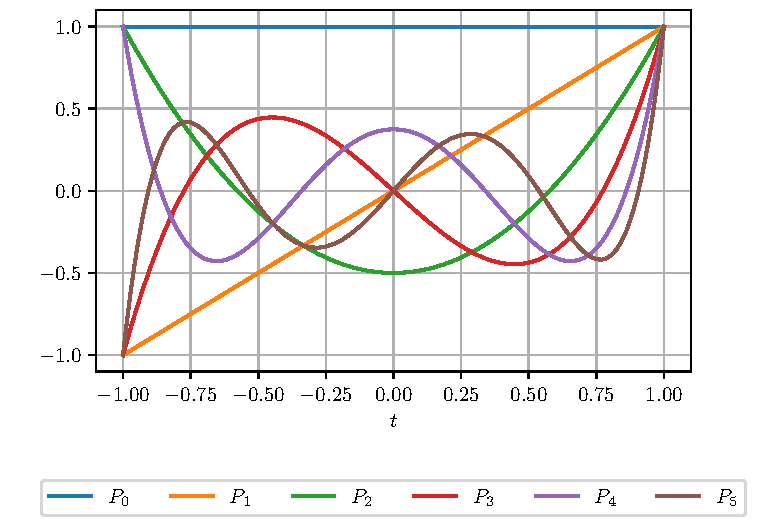
\includegraphics{./fig-legendre-polynomials.pdf}
\caption{Legendreove polynómy.  Obrázok bol pripravený Zdrojovým
kódom~\ref{src:lp} z~Prílohy~\ref{app:lp}.}
\label{fig:lp}
\end{figure}

V~Kapitole~\ref{sec:unit_vectors} sme ukázali, že ľubovoľný vektor $\vec r$
z~trojrozmerného pravouhlého súradnicového systému je možné popísať pomocou
jednotkových vektorov $\vec e_i$, $i = 1, 2, 3$.  Obdobne je možné pomocou
niektorých systémov funkcií popísať každú spojitú funkciu $f(t)$ na intervale
$t \in [1, 1]$.  Jeden z~takýchto systémov funkcií predstavujú práve
Legendreove polynómy~$P_n(t)$.

Rovnica
%
\begin{equation}
\label{eq:f_synthesis}
f(t) = \sum_{n = 0}^\infty \frac{2n + 1}{2} \, f_n \, P_n(t)
\end{equation}
%
umožňuje rozvinúť každú spojitú funkciu $f(t)$ do radu Legendreových polynómov
pre ľubovoľné $t \in [-1, 1]$.  Vzťah~(\ref{eq:f_synthesis}) je možné vnímať aj
ako analógiu vzťahu~(\ref{eq:r_synthesis}), pričom $f_n$ sú súradnice funkcie
$f(t)$ a~Legendreove polynómy $P_n(t)$ plnia podobnú úlohu ako jednotkové
vektory $\vec e_i$.  Konštanty $f_n$ sú dané skalárnym súčinom funkcií $f(t)$
a~$P_n(t)$ (porovnaj s~\ref{eq:r_analysis}),
%
\begin{equation}
\label{eq:f_analysis}
f_n = \int\limits_{-1}^1 f(t) \, P_n(t) \, \diff t{.}
\end{equation}
%
Dôkaz platnosti rovníc~(\ref{eq:f_synthesis}) a~(\ref{eq:f_analysis}) je možné 
nájsť napríklad vo \textcite{Freeden2009} či 
v~\textcite{SansoGeoidDetermination}.

Podobne ako skalárny súčin dvoch rôznych jednotkových vektorov $\vec e_i$ 
a $ \vec e_j$ je nulový (rovnica~\ref{eq:ei_orthogonality}), nulový je 
i~skalárny súčin dvoch rôznych Legendreovych polynómov $P_n(t)$ a $P_l(t)$,
%
\begin{equation}
\label{eq:lp_orthogonality}
\int\limits_{-1}^1 P_n(t) \, P_l(t) \, \diff t = 0{,} \quad n \neq l{.}
\end{equation}
%
Hovoríme preto, podobne ako v~súvislosti s~jednotkovými vektormi, že
\emph{Legendreove polynómy sú ortogonálne} na intervale $t \in [-1, 1].$
Rovnicu~(\ref{eq:lp_orthogonality}) možno zovšeobecniť doplnením prípadu $n
= l$ \parencite[napríklad][]{Hobson},
%
\begin{equation}
\label{eq:lp_orthogonality_2}
\int\limits_{-1}^1 P_n(t) \, P_l(t) \, \diff t = \frac{2}{2n + 1} \, 
\delta_{nl}{.}
\end{equation}

Rovnice~(\ref{eq:f_synthesis}) a~(\ref{eq:f_analysis}) sú vo fyzikálnej
geodézii veľmi často využívané a~v~istej miere sme sa s~nimi stretli už
v~predchádzajúcej kapitole.  Nech $r$ a~$r_Q$ z~rovnice~(\ref{eq:1l_legpol}) sú 
konštanty, pre ktoré platí $r > r_Q$ (pozri podmienku
$\alpha < 1$ v~rovnici~\ref{eq:generic_function_for_lps}).  Keď označíme $f(t)
= 1 \slash l(t)$, $t = \cos\psi$, pomocou rovníc~(\ref{eq:lp_orthogonality_2})
a~(\ref{eq:1l_legpol}) sa môžeme presvedčiť, že koeficienty $f_n$
z~rovnice~(\ref{eq:f_analysis}) sú dané vzťahom
%
\begin{equation}
f_n = \frac{1}{r_Q} \, \frac{2}{2n + 1} \, \left( \frac{r_Q}{r} \right)^{n
+ 1}{.}
\end{equation}
%
Dosadením týchto koeficientov do vzťahu~(\ref{eq:f_synthesis}) získame pôvodný 
vzťah~(\ref{eq:1l_legpol}).  Hoci ide o~triviálny príklad, demonštruje 
rozvinutie funkcie do radu Legendreových polynómov.  Takéto rozvinutie funkcie 
$f(t)$ pomocou Legendreových polynónom $P_n(t)$ je v~istom zmysle obdobné 
vyjadreniu vektora $\vec r$ pomocou jednotkových vektorov $\vec e_i$ 
z~Kapitoly~\ref{sec:unit_vectors}.  Tento rozvoj je v~mnohých situáciách 
výhodný, pretože môže napríklad zjednodušiť odvodenie.  Napokon, najlepšie to 
demonštruje azda samotná Kapitola~\ref{sec:vg_sh_expansion}, v~ktorej sme 
funkciu $1 \slash l$ rozvinuli do radu Legendreových polynómov a~následne 
Legendreových funkcií, čím sme získali vzťah~(\ref{eq:vg_sh_no_norm}).

Z~vlastností Legendreových polynómov spomeňme ešte aspoň nasledovné
\parencite{Freeden2009},
%
\begin{equation}
\label{eq:pn_property1}
P_n(1) = 1{,}
\end{equation}
%
\begin{equation}
\label{eq:pn_property2}
P_n(-t) = (-1)^n \, P_n(t){,}
\end{equation}
%
\begin{equation}
\label{eq:pn_property3}
|P_n(t)| \leq P_n(1) = 1{,} \quad t \in [-1, 1]{,}
\end{equation}
%
\begin{equation}
\label{eq:pn_property4}
P_n'(1) = \frac{n \, (n + 1)}{2}{,}
\end{equation}
%
kde $P_n'(t) = \diff P_n(t) \slash \diff t$.  Vzťahy~(\ref{eq:pn_property1}) až
(\ref{eq:pn_property4}) platia pre $n \geq 0$.   Širokú škálu ďalších
vlastností Legendreovych polynómov, ich derivácií či integrálov je možné nájsť
napríklad v~prácach \textcite{Gradshteyn2007}, \textcite{Freeden2009}
a~\textcite{Olver2010}.

Na záver pre úplnosť dodajme, že vzťahy~(\ref{eq:f_synthesis})
a~(\ref{eq:f_analysis}) možno aplikovať nielen na spojité funkcie $f(t)$ na
intervale $t \in [-1, 1]$, ale i~na širšiu množinu funkcií.  Podrobnosti možno
nájsť napríklad v~prácach \textcite{Freeden2009} či \textcite{Arfken2005}.






\section{Legendreove funkcie}
\label{sec:legendre_functions}

Dosadením Rodriguesovho vzorca~(\ref{eq:pn_rodrigues}) do~(\ref{eq:pnm_def})
získame vzťah pre Legendreove funkcie,
%
\begin{equation}
\label{eq:pnm_ferrer}
P_{nm}(t) = \frac{1}{2^n \, n!} (1 - t^2)^{ m \slash 2} \, \frac{\diff^{n + m}
(t^2 - 1)^n}{\diff t^{n + m}}{.}
\end{equation}
%
Existuje tiež explicitný vzťah \parencite{Freeden2009},
%
\begin{equation}
P_{nm}(t) = \frac{1}{2^n}(1 - t^2)^{m \slash 2} \sum_{s = 0}^{\left\lfloor
\frac{n - m}{2} \right\rfloor} (-1)^s \, \frac{(2n - 2s)!}{s! \, (n - s)! \, (n
- m - 2s)!} \, t^{n - m - 2s}{,}
\end{equation}
%
či
%
množstvo rekurentných vzorcov, napríklad \parencite{Freeden2009}
%
\begin{equation}
\label{eq:pnm_recurrence}
P_{nm}(t) = \frac{2n - 1}{n - m} \, t \, P_{n - 1, m}(t) + \frac{n + m - 1}{n
- m} \, P_{n - 2, m}(t){.}
\end{equation}
%
Niekoľko prvých Legendreových funkcií má nasledovný tvar
(Obrázok~\ref{fig:lf}),
%
\begin{equation}
\label{eq:lf00_to_lf22}
\begin{split}
P_{0,0}(t) & = 1{,}\\
P_{1,0}(t) & = t{,}\\
P_{1,1}(t) & = \sqrt{1 - t^2}{,}\\
P_{2,0}(t) & = \frac{1}{2}(3t^2 - 1){,}\\
P_{2,1}(t) & = 3t \, \sqrt{1 - t^2}{,}\\
P_{2,2}(t) & = 3(1 - t^2){.}\\
\end{split}
\end{equation}

\begin{figure}[bt]
\centering
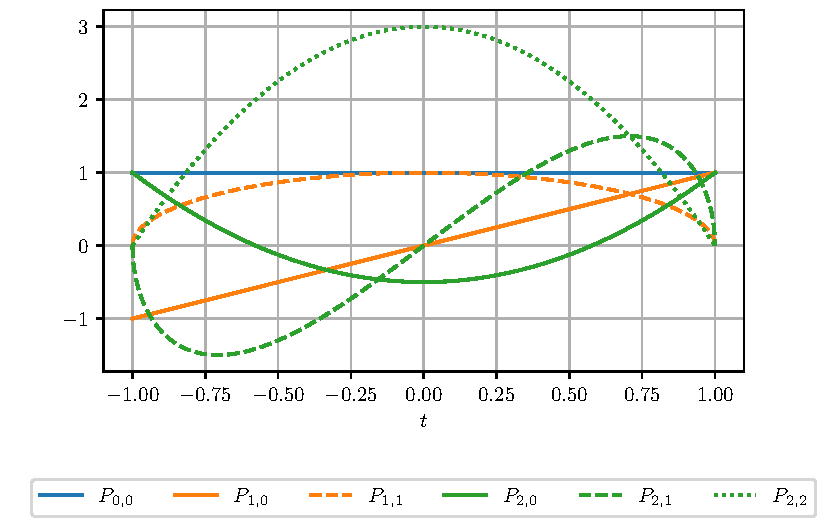
\includegraphics{./fig-legendre-functions.pdf}
\caption{Legendreove funkcie}
\label{fig:lf}
\end{figure}

Legendreove funkcie rôznych stupňov $n$, $l$ a~rovnakého rádu $m$ sú
ortogonálne \parencite{Freeden2009},
%
\begin{equation}
\label{eq:pnm_orthogonality}
\int\limits_{-1}^{1} P_{nm}(t) \, P_{lm}(t) \, \diff t = 0{,} \quad n \neq l{.}
\end{equation}
%
Pre dve Legendreove funkcie rovnakého stupňa a~rádu platí
\begin{equation}
\label{eq:pnm_times_pnm}
\int\limits_{-1}^{1} P^2_{nm}(t) \, \diff t = \frac{2}{2n + 1} \, \frac{(n 
+ m)!}{(n - m)!}{.}
\end{equation}

Legendreove funkcie vyhovujú diferenciálnej rovnici druhého rádu 
\parencite{SansoGeoidDetermination}
%
\begin{equation}
\label{eq:legfunc1_differential_equation}
(1 - t^2) \, \frac{\diff^2 P_{nm}(t)}{\diff t^2} - 2 \, t \, \frac{\diff 
P_{nm}(t)}{\diff t} + \left[ n \, (n + 1) - \frac{m^2}{1 - t^2} \right] \, 
P_{nm}(t) = 0{.}
\end{equation}
%
Rovnica~(\ref{eq:legfunc1_differential_equation}) sa nazýva \emph{Legendreova 
diferenciálna rovnica}.  Dosadením $m = 0$ 
do~(\ref{eq:legfunc1_differential_equation}) získame diferenciálnu rovnicu 
druhého rádu pre Legendreove polynómy,
%
\begin{equation}
\label{eq:legpol_differential_equation}
(1 - t^2) \, \frac{\diff^2 P_n(t)}{\diff t^2} - 2 \, t \, \frac{\diff 
P_n(t)}{\diff t} + n \, (n + 1) \, P_n(t) = 0{.}
\end{equation}

Na záver spomeňme ešte aspoň dve ďalšie vlastnosti Legendreových funkcií,
%
\begin{equation}
\label{eq:pnm_symmetry}
P_{nm}(-t) = (-1)^{n + m} \, P_{nm}(t)
\end{equation}
%
a
%
\begin{equation}
P_{nm}(\pm1) = 0{,} \quad m \neq 0{.}
\end{equation}

Numerický výpočet Legendreových funkcií je zvyčajne realizovaný rekurentnými 
vzťahmi.  Ide však o~netriviálnu úlohu, obzvlášť v~prípade vysokých stupňov 
a~rádov \parencite{Holmes2002a,Fukushima2012a,Ishioka2018}.  
Vlastnosť~(\ref{eq:pnm_symmetry}) je preto obzvlášť výhodná.  Ak potrebujeme 
vypočítať $P_{nm}(\sin\varphi)$ a~$P_{nm}(\sin(-\varphi))$, rekurentnými 
vzťahmi môžeme vypočítať iba jeden z~týchto členov, pričom druhý dopočítame 
jednoduchým vzťahom~(\ref{eq:pnm_symmetry}).

\subsection{Condonov--Shortleyho fázový faktor}
\label{sec:legendre_functions_cs_factor}

V geodézii a geomagnetizme sú Legendreove funkcie definované takmer výhradne 
vzťahom~(\ref{eq:pnm_ferrer}).  V~iných vedných odboroch, napríklad fyzike či 
seizmológii, sa však používa definícia, ktorá obsahuje člen $(-1)^m$ 
\parencite[pozri][]{Wieczorek2015,Olver2010},
%
\begin{equation}
\begin{split}
P_n^m(t) &= (-1)^m \, (1 - t^2)^{m \slash 2} \, \frac{\diff^m P_n(t)}{\diff 
t^m}\\
%
&= \frac{(-1)^m}{2^n \, n!} (1 - t^2)^{ m \slash 2} \, \frac{\diff^{n + m}
(t^2 - 1)^n}{\diff t^{n + m}}{.}
\end{split}
\end{equation}
%
V~takom prípade sa rád Legendreovej funkcie $m$ zvykne zapisovať do horného 
indexu.  Člen $(-1)^{m}$ sa nazýva Condonov--Shortleyho fázový faktor.  Medzi 
$P_{nm}(t)$ a $P_n^m(t)$ teda platí vzťah
%
\begin{equation}
P_{nm}(t) = (-1)^m \, P_n^m(t){.}
\end{equation}
%
V ďalších častiach práce budeme používať iba Legendreove funkcie $P_{nm}(t)$ 
definované vzťahom~(\ref{eq:pnm_ferrer}).




\section{Sférické harmonické funkcie}
\label{sec:spherical_harmonics}

V~rovnici~(\ref{eq:vg_sh_no_norm}) zaveďme substitúciu pre členy, ktoré závisia
iba od uhlovej časti sférických súradníc,
%
\begin{equation}
\label{eq:ynk_no_norm}
Y_{nk}(\varphi, \lambda) = P_{n|k|}(\sin\varphi)
%
\begin{cases}
\cos(k\lambda){,}    &\text{ak} \quad k \geq 0{,}\\
\sin(|k|\lambda){,}  &\text{ak} \quad k < 0{,}\\
\end{cases}
\end{equation}
%
pričom $n = 0, 1, 2, \dots$ a~$k = -n, \dots, n$.  Funkcia $Y_{nk}(\varphi,
\lambda)$ sa nazýva \emph{plošná sférická harmonická funkcia stupňa $n$ a~rádu
$k$}.

\begin{figure}[bt]
\centering
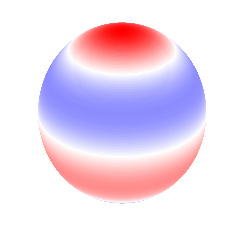
\includegraphics{./fig-spherical-harmonic-n3-k0.pdf}
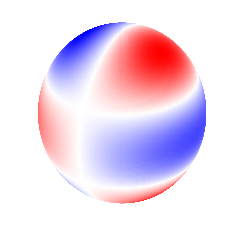
\includegraphics{./fig-spherical-harmonic-n3-k1.pdf}
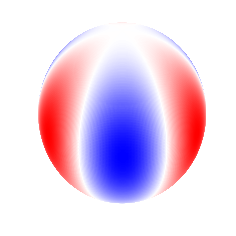
\includegraphics{./fig-spherical-harmonic-n3-k3.pdf}
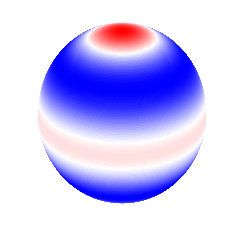
\includegraphics{./fig-spherical-harmonic-n4-k0.pdf}
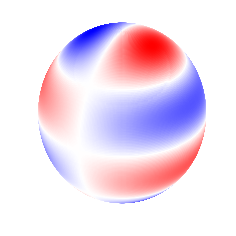
\includegraphics{./fig-spherical-harmonic-n4-k1.pdf}
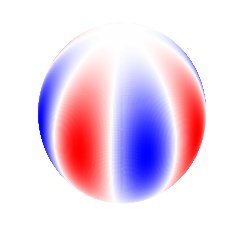
\includegraphics{./fig-spherical-harmonic-n4-k4.pdf}
\caption{Plošné sférické harmonické funkcie $Y_{nk}(\varphi, \lambda)$.
Záporné hodnoty sú zobrazené odtieňmi modrej farby, kladné hodnoty odtieňmi
červenej farby.  \textit{Vrchný rad} (zľava): $Y_{3,0}(\varphi, \lambda)$,
$Y_{3,1}(\varphi, \lambda)$, $Y_{3,3}(\varphi, \lambda)$.  \textit{Spodný rad}
(zľava): $Y_{4,0}(\varphi, \lambda)$, $Y_{4,1}(\varphi, \lambda)$,
$Y_{4,4}(\varphi, \lambda)$.  Obrázok bol pripravený Zdrojovým
kódom~\ref{src:ynk} z~Prílohy~\ref{app:sh}.}
\label{fig:sh}
\end{figure}

\begin{figure}[bt]
\centering
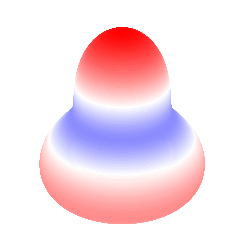
\includegraphics{./fig-spherical-harmonic-n3-k0-3d.pdf}
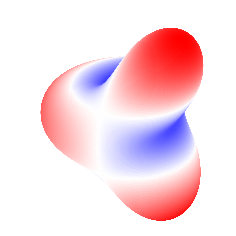
\includegraphics{./fig-spherical-harmonic-n3-k1-3d.pdf}
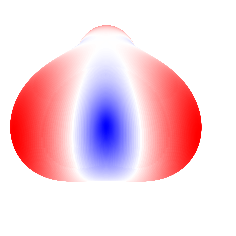
\includegraphics{./fig-spherical-harmonic-n3-k3-3d.pdf}
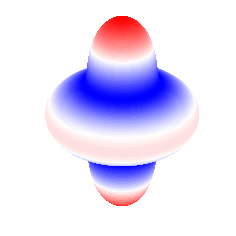
\includegraphics{./fig-spherical-harmonic-n4-k0-3d.pdf}
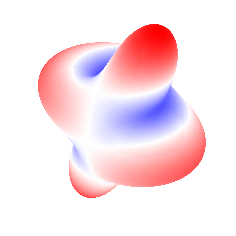
\includegraphics{./fig-spherical-harmonic-n4-k1-3d.pdf}
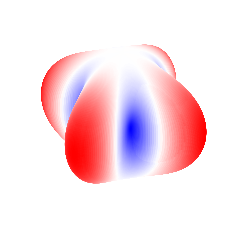
\includegraphics{./fig-spherical-harmonic-n4-k4-3d.pdf}
\caption{Plošné sférické harmonické funkcie $Y_{nk}(\varphi, \lambda)$
z~Obrázku~\ref{fig:sh} zobrazené odľahlosťou nadobúdanej hodnoty od jednotkovej
sféry.  Obrázok bol pripravený Zdrojovým kódom~\ref{src:ynk}
z~Prílohy~\ref{app:sh}.}
\label{fig:sh3d}
\end{figure}

Grafická reprezentácia sférických harmonických funkcií je uvedená na
Obrázkoch~\ref{fig:sh} a~\ref{fig:sh3d}.  Možno si všimnúť, že sférické
harmonické funkcie rádu $k = 0$ (ľavý stĺpec na obrázkoch) menia znamienko
v~smere sférickej šírky a~nezávisia od sférickej dĺžky.  Obe vlastnosti možno
overiť dosadením rádu $k = 0$ do rovnice~(\ref{eq:ynk_no_norm}),
%
\begin{equation}
\label{eq:yn0}
Y_{n0}(\varphi, \lambda) = P_n(\sin\varphi){.}
\end{equation}
%
Sférická harmonická funkcia $Y_{n0}(\varphi, \lambda)$ mení $n$-krát znamienko
v~smere sférickej šírky (porovnaj rovnicu~\ref{eq:yn0} a~Obrázok~\ref{fig:lp}).
Možno si tiež všimnúť, že parita stupňa $n$ určuje symetriu funkcie
$Y_{n0}(\varphi, \lambda)$ voči rovine rovníka; funkcia $Y_{n0}(\varphi,
\lambda)$ je symetrická voči rovine rovníka pre $n = 0, 2, 4, \dots$
a~nesymetrická pre $n = 1, 3, 5, \dots$ (pozri
Kapitolu~\ref{sec:legendre_polynomials}). Funkcie $Y_{n0}(\varphi, \lambda)$ sa
nazývajú \emph{zonálne sférické harmonické funkcie}.

Ak $0 < |k| < n$ (prostredný stĺpec na obrázkoch), sférická harmonická funkcia
mení znamienko s~oboma súradnicami.  V~smere sférickej šírky dochádza k~$n
- |k|$ zmenám znamienka.  Počet $n - |k|$ vyplýva zo skutočnosti, že
Legendreova funkcia $P_{n|k|}(\sin\varphi)$ súvisí s~$|k|$-tou deriváciou
Legendreovho polynómu $P_n(\sin\varphi)$ (pozri rovnice~\ref{eq:pnm_def}
a~\ref{eq:pnm_ferrer}).  Deriváciou polynómu sa znižuje jeho stupeň, a~teda aj
počet možností meniť znamienko.  V~smere sférickej dĺžky sa znamienko mení
$2|k|$-krát.  Táto hodnota vyplýva z~vlastností trigonometrických funkcií
$\cos(k\lambda)$ a~$\sin(|k|\lambda)$.  Sférická harmonická funkcia rádu $0
< |k| < n$ má prívlastok \emph{teserálna}.

Na záver, ak $|k| = n$ (pravý stĺpec na obrázkoch), sférická harmonická funkcia
mení znamienko $0$-krát v~smere sférickej šírky, pretože $n - |k| = n - n = 0$,
a~$2|k|$-krát v~smere sférickej dĺžky.  Takáto funkcia sa nazýva
\emph{sektorálna sférická harmonická funkcia}.

Podobne ako jednotkové vektory, Legendreove polynómy či niektoré Legendreove
funkcie, i~sférické harmonické funkcie sú ortogonálne.  Táto vlastnosť vyplýva
z~nulového skalárneho súčinu dvoch rôznych sférických harmonických funkcií
$Y_{nk}(\varphi, \lambda)$ a~$Y_{rs}(\varphi, \lambda)$,
%
\begin{equation}
\label{eq:ynk_no_norm_orthogonality}
\iint\limits_{\sigma} Y_{nk}(\varphi, \lambda) \, Y_{rs}(\varphi, \lambda) \, 
\diff \sigma = 0{,}
\end{equation}
%
pričom buď $n \neq r$ alebo $k \neq s$ alebo platia obe podmienky súčasne.  Pre
skalárny súčin dvoch rovnakých sférických harmonických funkcií platí
%
\begin{equation}
\label{eq:ynk_times_ynk}
\iint\limits_{\sigma} Y_{nk}(\varphi, \lambda) \, Y_{nk}(\varphi, \lambda) \, 
\diff \sigma =
%
\dfrac{4\pi}{(2 - \delta_{k0}) \, (2n + 1)} \, \dfrac{(n + |k|)!}{(n
- |k|)!}{.}
\end{equation}
%
Overenie vzťahov~(\ref{eq:ynk_no_norm_orthogonality})
a~(\ref{eq:ynk_times_ynk}) ponecháme na čitateľa.  Je potrebné použiť
rovnice~(\ref{eq:pnm_orthogonality}), (\ref{eq:pnm_times_pnm}),
(\ref{eq:ynk_no_norm}) a~vypočítať integrály
%
\begin{equation}
\int\limits_{0}^{2\pi} \cos(k \lambda) \, \diff\lambda \quad \text{a} \quad
\int\limits_{0}^{2\pi} \sin(|k| \lambda) \, \diff\lambda{.}
\end{equation}
%
Vo vzťahoch~(\ref{eq:pnm_orthogonality}) a~(\ref{eq:pnm_times_pnm}) je potrebné
aplikovať substitúciu integračnej premennej,
%
\begin{equation}
\int\limits_{-1}^{1} P_{nm}(t) \, P_{rs}(t) \, \diff
t~= \int\limits_{-\frac{\pi}{2}}^{\frac{\pi}{2}} P_{nm}(\sin\varphi) \,
P_{rs}(\sin\varphi) \, \cos\varphi \, \diff \varphi{.}
\end{equation}


Nech $f(\varphi, \lambda)$ je funkcia na jednotkovej sfére $\sigma$.  Nech pre
funkciu $f(\varphi, \lambda)$ ďalej platí nerovnosť
%
\begin{equation}
\label{eq:f_l2}
\iint\limits_\sigma f^2(\varphi, \lambda) \, \diff \sigma < \infty{.}
\end{equation}
%
Podmienku~(\ref{eq:f_l2}) spĺňa napríklad každá spojitá funkcia na jednotkovej
sfére.  Každú takúto funkciu $f(\varphi, \lambda)$ možno rozvinúť do radu
sférických harmonických funkcií \parencite[napríklad][]{MoritzPhysicalGeodesy},
%
\begin{equation}
\label{eq:f_shs_no_norm}
f(\varphi, \lambda) = \sum_{n = 0}^\infty \sum_{k = -n}^n f_{nk} \,
Y_{nk}(\varphi, \lambda){.}
\end{equation}
%
Koeficienty $f_{nk}$ je možné získať nasledovne.  Vynásobme 
rovnicu~(\ref{eq:f_shs_no_norm}) sférickou harmonickou funkciou 
$Y_{rs}(\varphi, \lambda)$ a~následne rovnicu zintegrujme na jednotkovej sfére 
$\sigma$.  Použitím vzťahov~(\ref{eq:ynk_no_norm_orthogonality}) 
a~(\ref{eq:ynk_times_ynk}) získame hľadané koeficienty
%
\begin{equation}
\label{eq:f_sha_no_norm}
f_{nk} = \frac{(2 - \delta_{k0}) \, (2n + 1)}{4\pi} \, \frac{(n - |k|)!}{(n 
+ |k|)!} \, \iint\limits_{\sigma} f(\varphi, \lambda) \, Y_{nk}(\varphi, 
\lambda) \, \diff \sigma{.}
\end{equation}
%

Vidíme teda, že ak funkcia $f(\varphi, \lambda)$ spĺňa
podmienku~(\ref{eq:f_l2}), potom možno pomocou sférických harmonických funkcií
túto funkciu rozložiť na jej súradnice $f_{nk}$
(rovnica~\ref{eq:f_sha_no_norm}) a~následne ju zrekonštruovať z~jej súradníc
(vzťah~\ref{eq:f_shs_no_norm}).  V~priestore funkcií $f(\varphi, \lambda)$,
ktoré sú definované na sfére a~spĺňajú podmienku~($\ref{eq:f_l2}$) plnia teda
sférické harmonické funkcie $Y_{nk}(\varphi, \lambda)$ podobnú úlohu ako plnia
jednotkové vektory $\vec e_i$ v~priestore trojrozmerných vektorov $\vec r$.
Funkcia $f(\varphi,\lambda)$ môže byť napríklad gravitačný či magnetický
potenciál telesa na sfére, ktorá obopína celé teleso, topografia Zeme či inej
planéty a~množstvo ďalších funkcií.  Každú takúto funkciu možno rozvinúť do
vlastného radu sférických harmonických funkcií (vzťah~\ref{eq:f_shs_no_norm}),
pričom každá funkcia bude mať vlastné súradnice $f_{nk}$, podobne ako každý
vektor $\vec r$ má vlastné súradnice $r_i$.  Všimnime si, že ak označíme
%
\begin{equation}
\label{eq:sh_norm}
N_{n|k|} = \sqrt{(2 - \delta_{k0}) (2n + 1) \, \frac{(n - |k|)!}{(n
+ |k|)!}}{,}
\end{equation}
%
potom vzťahy~(\ref{eq:f_sha_no_norm}) a~(\ref{eq:f_shs_no_norm}) sú totožné so
vzťahmi~(\ref{eq:vg_analysis}) a~(\ref{eq:vg_synthesis}) pre $r = 1$.



\section{Normovanie}
\label{sec:normalization}

V~praktických aplikáciách sa sférické harmonické funkcie zvyknú definovať tak, 
že sú vynásobené členom, ktorý závisí od sférického harmonického stupňa a rádu.  
Tento člen sa nazýva \emph{norma} a~jeho použitím dostaneme \emph{normované} 
sférické harmonické funkcie.  Normovaním získame niektoré vlastnosti, ktoré sú 
výhodne z~teoretického aj z~praktického hľadiska.  Tieto vlastnosti budú 
podrobnejšie diskutované v~Kapitolách~\ref{sec:leg_sh_norm} 
a~\ref{sec:shc_norm}.  Existuje niekoľko typov noriem, napríklad Schmidtova 
polovičná norma, ortogonálna norma či úplná norma \parencite{SHTOOLS}.  
V~geodézii sa používa takmer výhradne posledná menovaná norma, preto sa 
ostatným normám nebudeme v~tejto práci venovať.

\subsection{Legendreove funkcie a~sférické harmonické funkcie}
\label{sec:leg_sh_norm}

Pre skalárny súčin dvoch rovnakých jednotkových vektorov $\vec e_i$ platí 
vzťah~(\ref{eq:ei_unit_length}).  Z~teoretického aj z~praktického hľadiska by 
bolo výhodné, aby aj skalárny súčin dvoch rovnakých sférických harmonických 
funkcií bol rovný~$1$.  Túto vlastnosť možno zabezpečiť vynásobením 
Legendreových funkcií $P_{nm}(\sin\varphi)$ členom $N_{n|k|}$ 
(rovnica~\ref{eq:sh_norm}), ktorý nazývame \emph{úplná norma}.  Získame tým 
\emph{úplne normované Legendreove funkcie},
%
\begin{equation}
\bar{P}_{nm}(\varphi) = N_{nm} \, P_{nm}(\varphi){,} \quad  n = 0, 1, \dots,
\quad m = 0, 1, \dots, n{,}
\end{equation}
%
a~\emph{úplne normované sférické harmonické funkcie}
%
\begin{equation}
\label{eq:ynk_norm}
\begin{split}
\bar{Y}_{nk}(\varphi, \lambda) = N_{n|k|} \, Y_{nk}(\varphi, \lambda)
= \bar{P}_{n|k|}(\sin\varphi)
%
\begin{cases}
\cos(k\lambda){,}    &\text{ak} \quad k \geq 0{,}\\
\sin(|k|\lambda){,}  &\text{ak} \quad k < 0{,}
\end{cases}
&
%
\\
n = 0, 1, \dots, \quad k = -n, \dots, n{.}&
\end{split}
\end{equation}
%
Použitím normy~(\ref{eq:sh_norm}) je možné obdobne ako v~prípade
rovnice~(\ref{eq:ynk_no_norm_orthogonality}) ukázať, že platí
%
\begin{equation}
\label{eq:ynk_norm_orthogonality}
\frac{1}{4\pi} \, \iint\limits_{\sigma} \bar{Y}_{nk}(\varphi, \lambda) \,
\bar{Y}_{rs}(\varphi, \lambda) \, \diff \sigma = \delta_{nr} \, \delta_{ks}{.}
\end{equation}
%
Skalárny súčin~(\ref{eq:ynk_norm_orthogonality}) dvoch rôznych úplne
normovaných sférických harmonických funkcií je teda rovný 0, zatiaľ čo skalárny
súčin dvoch rovnakých úplne normovaných sférických harmonických funkcií je
rovný $1$.

Vzťahy~(\ref{eq:f_shs_no_norm}) a~(\ref{eq:f_sha_no_norm}) potom prejdu do
tvaru
%
\begin{equation}
\label{eq:f_shs}
f(\varphi, \lambda) = \sum_{n = 0}^\infty \sum_{k = -n}^n \bar{f}_{nk} \,
\bar{Y}_{nk}(\varphi, \lambda)
\end{equation}
%
a
%
\begin{equation}
\label{eq:f_sha}
\bar{f}_{nk} = \frac{1}{4\pi} \, \iint\limits_{\sigma} f(\varphi, \lambda) \,
\bar{Y}_{nk}(\varphi, \lambda) \, \diff \sigma{.}
\end{equation}
%
Úplne normované sférické harmonické funkcie tiež umožňujú zapísať dekompozičný
teorém~(\ref{eq:pn_decomposition_formula}) v~tvare
\parencite{MoritzPhysicalGeodesy}
%
\begin{equation}
P_n(\cos\psi) = \frac{1}{2n + 1} \, \sum_{k = -n}^n \bar{Y}_{nk}(\varphi,
\lambda) \, \bar{Y}_{nk}(\varphi_Q, \lambda_Q)
\end{equation}
%
a~prevrátenú hodnotu vzdialenosti $1 \slash l$ z~rovnice~(\ref{eq:1l}) v~tvare
%
\begin{equation}
\label{eq:1l_sh}
\frac{1}{l} = \frac{1}{r_Q} \, \sum_{n = 0}^{\infty} \frac{1}{2n + 1} \, \left( 
\frac{r_Q}{r} \right)^{n + 1} \, \sum_{k = -n}^n \bar{Y}_{nk}(\varphi,
\lambda) \, \bar{Y}_{nk}(\varphi_Q, \lambda_Q){.}
\end{equation}
%

Z~numerického hľadiska je výpočet nenormovaných Legendreových funkcií 
problematický, a~to už i~pre stupne a~rády presahujúce niekoľko stoviek.  
Dôvodom je ich pomerne rýchlo narastajúca hodnota, ktorá dokonca prekročí 
rozsah dvojitej presnosti.  Dvojitá presnosť je v~súčasnosti najčastejšie 
používaný štandard na počítačovú reprezentáciu čísel s~pohyblivou desatinnou 
čiarkou.  Číslo väčšie ako horný rozsah dvojitej presnosti je v~dvojitej 
presnosti reprezentované nekonečnom.  Z~tohto dôvodu je z~praktického hľadiska 
výhodnejšie pracovať s~úplne normovanými Legendreovými funkciami.  Kvôli 
opísaným numerickým problémom sa však nepočíta zvlášť norma $N_{nm}$ a~zvlášť 
nenormované Legendreove funkcie $P_{nm}(\sin\varphi)$, ale počítajú sa priamo 
úplne normované Legendreove funkcie $\bar{P}_{nm}(\sin\varphi)$ pomocou 
upravených rekurentných vzťahov (pozri napríklad \cite{Holmes2002a} či 
\cite{Fukushima2012a}).



\subsection{Sférické harmonické koeficienty}
\label{sec:shc_norm}

Sférické harmonické koeficienty $C_{nm}$ a~$S_{nm}$ zo
vzťahu~(\ref{eq:vg_sh_no_norm}) sú zvyčajne normované dvakrát.  Prvá norma
zabezpečí, že budú bezrozmerné, druhá norma je daná vzťahom~(\ref{eq:sh_norm}).

Fyzikálna jednotka koeficientov $C_{nm}$ a~$S_{nm}$
z~rovnice~(\ref{eq:vg_shc_no_norm}) je $\mathrm{m}^n \, \mathrm{kg}$, teda
závisí od stupňa $n$.  Je preto výhodne koeficienty normovať tak, aby boli
bezrozmerné.  Norma zaužívaná v~geodézii má tvar
%
\begin{equation}
\begin{rcases}
\tilde{C}_{nm}\\
\tilde{S}_{nm}
\end{rcases}
= \frac{1}{M \, R^n}
\begin{cases}
C_{nm}{,}\\
S_{nm}{,}
\end{cases}
\end{equation}
%
kde $M$ je hmotnosť telesa, ktoré generuje gravitačný potenciál a~$R$ je
polomer najmenšej sféry, v~ktorej sa celé teleso nachádza, teda $R
= \max(r_\mathrm{S}(\varphi_Q, \lambda_Q))$.  Vzťah~(\ref{eq:vg_sh_no_norm})
potom prejde do tvaru
%
\begin{equation}
\label{eq:vg_sh_1st_norm}
V_\gidx(P) = \frac{GM}{R} \sum_{n = 0}^\infty \left( \frac{R}{r} \right)^{n
+ 1} \sum_{m = 0}^{n} \left( \tilde{C}_{nm} \, \cos(m\lambda) + \tilde{S}_{nm}
\, \sin(m\lambda)\right) \, P_{nm}(\sin\varphi){.}
\end{equation}

Ak majú byť použité sférické harmonické funkcie normované členom $N_{n|k|}$,
potom sférické harmonické koeficienty musia byť normou $N_{n|k|}$ vydelené, aby
sa zachovala rovnosť vo vzťahoch~(\ref{eq:vg_sh_no_norm})
a~(\ref{eq:vg_sh_1st_norm}).  Druhá norma sférických harmonických koeficientov
je preto daná nasledovne,
%
\begin{equation}
\begin{rcases}
\bar{C}_{nm}\\
\bar{S}_{nm}
\end{rcases}
= \frac{1}{N_{nm}}
\begin{cases}
\tilde{C}_{nm}{,}\\
\tilde{S}_{nm}{.}
\end{cases}
\end{equation}
%
Sférický harmonický rozvoj~(\ref{eq:vg_sh_1st_norm}) následne prejde do tvaru
%
\begin{equation}
\label{eq:vg_sh_2nd_norm}
V_\gidx(P) = \frac{GM}{R} \sum_{n = 0}^\infty \left( \frac{R}{r} \right)^{n
+ 1} \sum_{m = 0}^{n} \left( \bar{C}_{nm} \, \cos(m\lambda) + \bar{S}_{nm} \,
\sin(m\lambda)\right) \, \bar{P}_{nm}(\sin\varphi){.}
\end{equation}
%
Ekvivalentný, no úspornejší zápis dosiahneme použitím substitúcie
$\bar{Y}_{nk}(\varphi, \lambda)$,
%
\begin{equation}
\label{eq:vg_sh_2nd_norm_ynk}
V_\gidx(P) = \frac{GM}{R} \sum_{n = 0}^\infty \left( \frac{R}{r} \right)^{n
+ 1} \sum_{k = -n}^{n} \bar{v}_{nk} \, \bar{Y}_{nk}(\varphi, \lambda){,}
\end{equation}
kde
%
\begin{equation}
\bar{v}_{nk} =
%
\begin{cases}
\bar{C}_{nk}{,}    &\text{ak} \quad k \geq 0{,}\\
\bar{S}_{n|k|}{,}  &\text{ak} \quad k < 0{.}\\
\end{cases}
\end{equation}
%
Koeficienty $\bar{C}_{nm}$ a~$\bar{S}_{nm}$, resp. $\bar{v}_{nk}$, sa nazývajú
\emph{úplne normované sférické harmonické koeficienty}.

Podobne ako v~prípade úplne normovaných Legendreových funkcií, ani sférické
harmonické koeficienty sa nezvyknú počítať samostatne od normy.  Namiesto toho
sa vypočítajú úplne normované sférické harmonické funkcie
$\bar{Y}_{nk}(\varphi, \lambda)$ a~následne sa napríklad
vzťahom~(\ref{eq:f_sha}) získajú priamo úplne normované sférické harmonické
koeficienty.





% -----------------------------------------------------------------------------

\section{Fyzikálnych význam niektorých sférických harmonických koeficientov}
\label{sec:physical_meaning_of_spherical_harmonic_coefficients}

Dosaďme $P_{0,0}(\sin\varphi)$ z~rovnice~(\ref{eq:lf00_to_lf22})
do rovnice~(\ref{eq:vg_shc_no_norm}) pre $n = 0$ a~$m = 0$,
%
\begin{equation}
C_{0,0} = \iiint\limits_{\tau} \rho(Q) \, \diff \tau(Q) = M{.}
\end{equation}
%
Nenormovaný koeficient $C_{0,0}$ má teda fyzikálny význam, je rovný hmotnosti 
telesa~$M$.  Ak obmedzíme nekonečné rady~(\ref{eq:vg_sh_no_norm}), 
(\ref{eq:vg_sh_1st_norm}), (\ref{eq:vg_sh_2nd_norm}) či 
(\ref{eq:vg_sh_2nd_norm_ynk}) na maximálny stupeň $N = 0$, získame vzťah
%
\begin{equation}
\label{eq:vg_sh_0degree}
V_\gidx(P) = \frac{GM}{r}{.}
\end{equation}
%
Rovnica~(\ref{eq:vg_sh_0degree}) predstavuje gravitačný potenciál hmotného bodu
s~hmotnosťou $M$ vo vzdialenosti $r$ od hmotného bodu (pozri
rovnicu~\ref{eq:vg_point_mass}).  Pomocou Newtonovho
integrálu~(\ref{eq:vg_body}) možno ukázať, že gravitačný potenciál gule
s~konštantnou hustotou (homogénna guľa) je tiež ekvivalentný so
vzťahom~(\ref{eq:vg_sh_0degree}).  Ak teda obmedzíme nekonečný sférický
harmonický rozvoj gravitačného potenciálu na maximálny stupeň $N = 0$, získame
gravitačný potenciál homogénnej gule, ktorá nahrádza skutočné teleso.

Vydeľme rovnicu~(\ref{eq:vg_shc_no_norm}) hmotnosťou $M$ a~zopakujme postup pre
stupeň $n = 1$ a~rády $m = 0, 1$.  Po uvážení~(\ref{eq:sph2cart}) získame
%
\begin{equation}
\begin{split}
\frac{C_{1,0}}{M} &= \frac{1}{M} \iiint\limits_{\tau} \rho(Q) \, z_Q \, \diff 
\tau(Q) = z_\mathrm{c}{,}\\
\frac{C_{1,1}}{M} &= \frac{1}{M} \iiint\limits_{\tau} \rho(Q) \, x_Q \, \diff 
\tau(Q) = x_\mathrm{c}{,}\\
\frac{S_{1,1}}{M} &= \frac{1}{M} \iiint\limits_{\tau} \rho(Q) \, y_Q \, \diff 
\tau(Q) = y_\mathrm{c}{.}
\end{split}
\end{equation}
%
Súradnice $x_\mathrm{c}$, $y_\mathrm{c}$ a~$z_\mathrm{c}$ predstavujú posun
začiatku súradnicového systému voči ťažisku telesa.  V~prípade gravitačného
poľa Zeme veľmi často pracujeme v~geocentrickom súradnicovom systéme so
začiatkom v~ťažisku Zeme, preto všetky koeficienty stupňa $n = 1$ sú zvyčajne
nulové, $C_{1,0} = C_{1,1} = S_{1,1} = 0$.

Je možné ukázať \parencite[napríklad][]{MoritzPhysicalGeodesy}, že koeficienty
stupňa $n = 2$ súvisia s~momentom zotrvačnosti.  Koeficienty vyšších stupňov
už, zdá sa, nemajú priamočiaru fyzikálnu interpretáciu.






% -----------------------------------------------------------------------------

\section{Aplikácie sférického harmonického rozvoja}
\label{sec:spherical_harmonics_applications}

Z~predchádzajúcich kapitol vieme, že gravitačný potenciál skutočnej Zeme je
možné vypočítať vzťahom~(\ref{eq:vg_sh_2nd_norm}).  Na takýto výpočet je
potrebné poznať sférické harmonické koeficienty $\bar{C}_{nm}$
a~$\bar{S}_{nm}$.

Koeficienty $\bar{C}_{nm}$ a~$\bar{S}_{nm}$ je možné vypočítať napríklad
z~obežnej dráhy umelej družice Zeme.  Tak ako Slnko ovplyvňuje dráhu planéty
v~príklade z~Kapitoly~\ref{sec:newton_law}, podobne i~Zem vplýva na dráhu
družice prostredníctvom svojho gravitačného poľa.  Tentokrát je ale situácia
zložitejšia ako na Obrázku~\ref{fig:orbital_motion}, pretože družica obieha
okolo Zeme v~bezprostrednej blízkosti vo výške približne $250$~-- $500$~km nad
jej povrchom.  Keďže gravitačné pole Zeme sa v~priestore rôznorodo mení (pozri
Obrázky~\ref{fig:gg_grav_sr_2arcsec} a~\ref{fig:vg_grav_sr_2arcsec}), dráha
družice je ovplyvnená ináč v~oblasti so silným gravitačným poľom (napríklad nad
masívnymi pohoriami) a~ináč v~oblasti so slabším gravitačným poľom.  V~dôsledku
premenlivého gravitačného poľa Zeme preto družica neobieha po
elipse.\footnote{Dráhu družice ovplyvňujú aj iné faktory, napríklad tlak
slnečného žiarenia, odpor atmosféry a~pod.  Tieto vplyvy pre jednoduchosť
zanedbáme.}  Jej skutočná dráha je komplikovaná priestorová krivka,
reflektujúca gravitačné pole v~danej oblasti, a~elipsa je len jej priblíženie
(Obrázok~\ref{fig:orbital_motion_real}).  Ak by sme teda poznali skutočnú dráhu
družice, mali by sme byť schopní inverzným spôsobom vypočítať to pole, ktoré je
príčinou neeliptickej dráhy.  Inými slovami, zo skutočnej dráhy družice je
možné vypočítať sférické harmonické koeficienty $\bar{C}_{nm}$
a~$\bar{S}_{nm}$.  Koeficienty $\bar{C}_{nm}$ a~$\bar{S}_{nm}$ je možné
vypočítať i~z mnohých iných geodetických meraní, či už družicových alebo
pozemných.  Podrobnejšie informácie o~družicových misiách a~jednotlivých
technikách je možné nájsť napríklad v~prácach \textcite{SeeberSatelliteGeodesy}
a~\textcite{MoritzPhysicalGeodesy}.

\begin{figure}
\centering
\input{./fig-orbital-motion-real.pdf_tex}
\caption{Pohyb umelej družice Zeme}
\label{fig:orbital_motion_real}
\end{figure}

ICGEM (angl. \emph{International Centre for Global Earth Models}) je služba 
zriadená Medzinárodnou geodetickou asociáciou (angl. \emph{International 
Association of Geodesy}, IAG).  Okrem iného je jej cieľom zbierať, archivovať 
a~poskytovať globálne modely gravitačného poľa Zeme, najčastejšie práve vo 
forme sférických harmonických koeficientov $\bar{C}_{nm}$ a~$\bar{S}_{nm}$.  Na 
domovskej stránke služby možné nájsť desiatky sád sférických harmonických 
koeficientov, získané z~rôznych dát a~rozličnými metódami 
výpočtu.\footnote{\url{http://icgem.gfz-potsdam.de/home}} je  Dostupné sú aj 
časovo premenlivé modely gravitačného poľa, služba na výpočet 
vzťahu~(\ref{eq:vg_sh_2nd_norm}) či modely gravitačného poľa nebeských telies 
(napríklad Mars, Venuša, Mesiac či asteroidy Slnečnej sústavy).

V~Kapitolách~\ref{sec:vg} a~\ref{sec:potential_theory} sme uviedli, že
v~gravitačnom potenciáli $V_\gidx$ je obsiahnutá informácia o~celom gravitačnom
poli.  Zo vzťahu~(\ref{eq:vg_sh_2nd_norm}) je preto možné vyťažiť oveľa viac
ako len informáciu o~gravitačnom potenciáli.  Napríklad aplikovaním operátora 
gradient~(\ref{eq:gradient_sph}) na gravitačný 
potenciál~(\ref{eq:vg_sh_2nd_norm}) možno získať prvky vektora gravitačného 
zrýchlenia v~lokálnom pravouhlom súradnicovom systéme s~pohyblivým začiatkom 
(Obrázok~\ref{fig:cart_sph}),
%
\begin{align}
\label{eq:vgx_sh}
\frac{\partial V_\gidx(P)}{\partial x^\mathrm{s}} &= \frac{1}{r} \, 
\frac{\partial V_\gidx(P)}{\partial \varphi}\nonumber\\
%
&= \frac{GM}{R^2} \sum_{n = 0}^\infty \left( \frac{R}{r} \right)^{n + 2} 
\sum_{m = 0}^{n} \left(
\bar{C}_{nm} \, \cos(m\lambda) + \bar{S}_{nm} \, \sin(m\lambda)\right) \,
\frac{\diff \bar{P}_{nm}(\sin\varphi)}{\diff \varphi}{,}\\
%
\label{eq:vgy_sh}
\frac{\partial V_\gidx(P)}{\partial y^\mathrm{s}} &= \frac{1}{r \, \cos\varphi} 
\, \frac{\partial V_\gidx(P)}{\partial \lambda}\nonumber\\
%
&= \frac{GM}{R^2 \, \cos\varphi} \sum_{n = 0}^\infty \left( \frac{R}{r} 
\right)^{n + 2} \sum_{m = 0}^{n}\left(
\bar{S}_{nm} \, \cos(m\lambda) - \bar{C}_{nm} \, \sin(m\lambda)\right) \, m \,
\bar{P}_{nm}(\sin\varphi){,}\\
%
\label{eq:vgz_sh}
\frac{\partial V_\gidx(P)}{\partial z^\mathrm{s}} &= \frac{\partial 
V_\gidx(P)}{\partial r}\nonumber\\
%
&= - \frac{GM}{R^2} \sum_{n = 0}^\infty (n + 1) \, \left( \frac{R}{r} 
\right)^{n + 2} \sum_{m = 0}^{n}
\left( \bar{C}_{nm} \, \cos(m\lambda) + \bar{S}_{nm} \, \sin(m\lambda)\right)
\, \bar{P}_{nm}(\sin\varphi){.}
\end{align}
%
Sférickými harmonickými rozvojmi teda môžeme vypočítať prakticky akúkoľvek 
veličinu gravitačného či tiažového poľa, od gravitačného potenciálu, cez 
gravitačné zrýchlenie až po zvislicové odchýlky či geoid.  
Rovnice~(\ref{eq:vgx_sh}) až~(\ref{eq:vgz_sh}) tiež prakticky demonštrujú, aké 
výhodné je poznať tvar operátora gradient vo sférických súradniciach 
(rovnica~\ref{eq:gradient_sph}).  Priamy výpočet derivácií $\partial V_\gidx 
\slash \partial x^\mathrm{s}$, $\partial V_\gidx \slash \partial y^\mathrm{s}$ 
a $\partial V_\gidx \slash \partial z^\mathrm{s}$ 
vzťahu~(\ref{eq:vg_sh_2nd_norm}) by bol totižto náročný.

Sférické harmonické koeficienty gravitačného poľa Zeme sú v~súčasnosti dostupné
približne do stupňa $2190$.  Získavané sú väčšinou kombináciou družicových
meraní (približne do stupňa $250$ až $300$) a~detailných pozemných
gravimetrických meraní (približne do stupňa $720$ až $2190$).  Existujú tiež 
modely, ktoré popisujú zemské gravitačné pole do vyšších stupňov ako $2190$.  
Tieto vysoké harmonické stupne však nie sú založené na meraniach zemského 
gravitačného poľa, ale na modelovaní gravitačného účinku topografických hmôt, 
ktoré sa nachádzajú nad geoidom \parencite{Ince2020}.

\begin{figure}
\centering
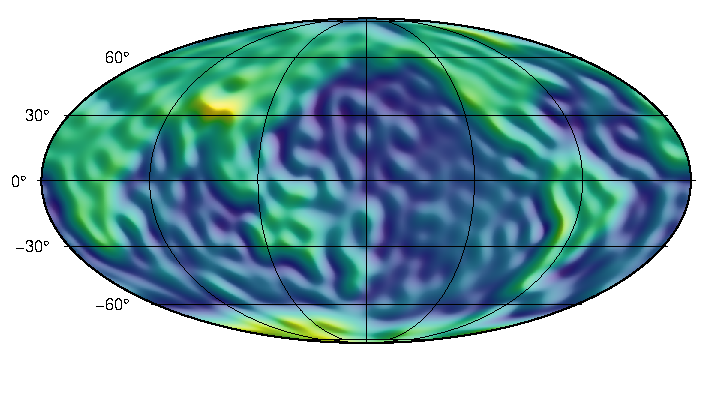
\includegraphics{./fig-h-shs-nmax30.pdf}
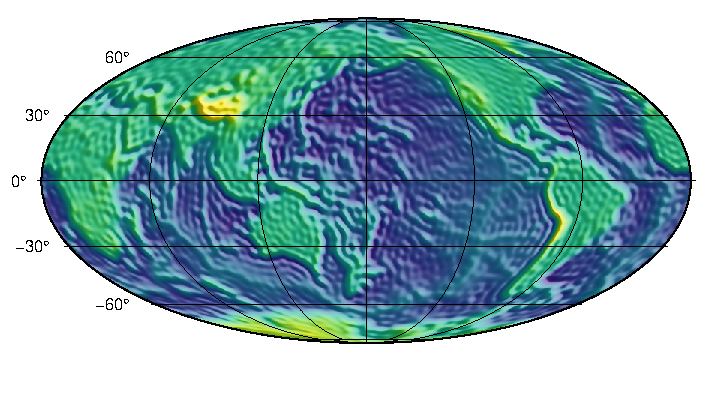
\includegraphics{./fig-h-shs-nmax90.pdf}
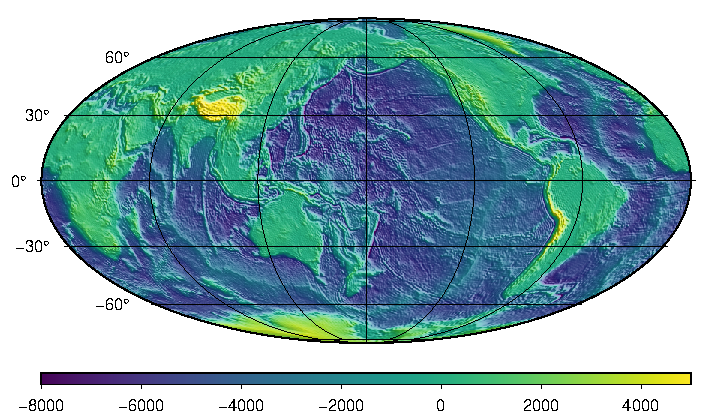
\includegraphics{./fig-h-shs-nmax360.pdf}
\caption{Sférický harmonický rozvoj zemskej topografie do stupňov~$N = 30$
(vrchná mapa), $90$~ (prostredná mapa) a~$360$~(spodná mapa).  Výpočet bol
uskutočnený Zdrojovým kódom~\ref{src:h_shs}.}
\label{fig:shs_h}
\end{figure}

V~Kapitole~\ref{sec:spherical_harmonics} sme uviedli, že do radu sférických
harmonických funkcií je možné rozvinúť nielen gravitačný potenciál, ale každú
funkciu, ktorá spĺňa podmienku~\ref{eq:f_l2}.  Rozviňme teda zemskú topografiu
$H(\varphi, \lambda)$ do maximálneho stupňa $N$,
%
\begin{equation}
\label{eq:h_shs}
H(\varphi, \lambda) = \sum_{n = 0}^{N} \sum_{k = -n}^n \bar{h}_{nk} \,
\bar{Y}_{nk}(\varphi, \lambda){.}
\end{equation}
%
Obrázok~\ref{fig:shs_h} znázorňuje vplyv parametra~$N$ na priestorové
rozlíšenie funkcie $H(\varphi, \lambda)$.  Hoci všetky tri mapy sú vypočítané
s~rovnakým vzorkovaním $0.25^{\circ}$ vo sférickej šírke a~dĺžke, spodná mapa
poskytuje vyššiu mieru detailu ako dve mapy nad ňou.  Je to spôsobené tým, že
maximálny stupeň $N$ udáva maximálne priestorové rozlíšenie funkcie
$H(\varphi,\lambda)$.  Polovica najkratšej vlnovej dĺžky funkcie sférického
harmonického rozvoja do stupňa $N$ je daná vzťahom
%
\begin{equation}
l_{\min}(N) = \frac{\pi \, R}{N}{,}
\end{equation}
%
kde $l_{\min}$ je sférická vzdialenosť v~dĺžkových jednotkách na sfére 
s~polomerom $R$.  Zvyšovaním
maximálneho stupňa $N$ teda zvyšujeme podrobnosť funkcie $H(\varphi, \lambda)$.







% -----------------------------------------------------------------------------

\section{Konvergencia sférického harmonického rozvoja na povrchu Zeme}
\label{sec:convergence_of_spherical_harmonics}

Pred rozvinutím generickej funkcie pre Legendreove polynómy do Maclaurinovho 
radu (vzťah~\ref{eq:maclaurin_series_of_generic_function}) sme vyslovili 
predpoklad $\frac{r_Q}{r} < 1$.  Bez splnenia tejto podmienky 
rad~(\ref{eq:maclaurin_series_of_generic_function}) nemusí konvergovať.  
V~takom prípade nie je možné pokračovať v~odvodení 
z~Kapitoly~\ref{sec:vg_sh_expansion}.  Ak totiž 
rad~(\ref{eq:maclaurin_series_of_generic_function}) diverguje, zámena poradia 
integrácie a~sumácie nie je možná.  Na získanie vzťahu~(\ref{eq:vg_sh_no_norm}) 
sme preto museli predpokladať, že podmienka $\frac{r_Q}{r} < 1$ je splnená.

\begin{figure}
\centering
\input{./fig-spherical-harmonics-convergence.pdf_tex}
\caption{Sférický harmonický rad~(\ref{eq:vg_sh_no_norm}) konverguje rovnomerne 
a~absolútne vo vonkajšom priestore sféry konvergencie.  Svetlosivá farba 
označuje oblasť, v~ktorej nie je zaručená konvergencia.  Tmavosivá farba 
predstavuje hmoty telesa, ktoré generuje gravitačné pole.  V~tejto oblasti 
rad~(\ref{eq:vg_sh_no_norm}) nepopisuje skutočný gravitačný potenciál.}
\label{fig:spherical_harmonics_convergence}
\end{figure}

Nerovnosť $\frac{r_Q}{r} < 1$ môžeme prepísať do tvaru $r > r_Q$.  Táto
nerovnosť je splnená pre \emph{všetky} diferenciálne elementy $\diff \tau(r_Q,
\varphi_Q, \lambda_Q)$ iba vtedy, ak pre sprievodič $r$ výpočtového bodu $P(r,
\varphi, \lambda)$ platí
%
\begin{equation}
\label{eq:spherical_harmonic_convergence}
r > \max(r_Q) = R{,}
\end{equation}
%
kde $R$ je sprievodič najvzdialenejšieho diferenciálneho elementu $\diff\tau$ 
od začiatku súradnicového systému.  Sféra s~polomerom $R$ sa nazýva sféra 
konvergencie \parencite{Hotine} 
(Obrázok~\ref{fig:spherical_harmonics_convergence}).  Vo vonkajšom priestore 
sféry konvergencie rad~(\ref{eq:vg_sh_no_norm}) konverguje rovnomerne 
a~absolútne.  Na tejto sfére ani v~jej vnútri konvergencia zaručená nie je.

Nanešťastie, celý povrch Zeme sa nachádza v~oblasti, v~ktorej sférický 
harmonický rozvoj gravitačného potenciálu nemusí konvergovať.  Našťastie, zdá 
sa, že otázka konvergencie, resp. divergencie radu~(\ref{eq:vg_sh_no_norm}) nie 
je v~súčasnosti z~praktického hľadiska relevantná pre nízke až stredné stupne 
a~svoju závažnosť nadobúda až približne od stupňa $10{,}800$ 
\parencite{Hirt2016,Rexer2017}.

Konvergencia radu sférických harmonických funkcií na povrchu Zeme je často 
diskutovanou témou geodetickej literatúry 
\parencite{Hotine,Krarup1969,MoritzAdvancedGeodesy,Sjoberg1980,Jekeli1983,SansoGeoidDetermination}.






% -----------------------------------------------------------------------------

\chapter{Sféroidický harmonický rozvoj}

V~niektorých situáciách je potrebné skúmať gravitačné pole sploštených telies.  
Príkladom splošteného telesa je samotná Zem či mnohé asteroidy Slnečnej sústavy 
(napríklad Eros, Castalia či Bennu; pozri \cite{Garmier2001}, \cite{Hu2015}, 
\cite{Sebera2016} či \cite{Reimond2016}).  Ak by sme rozvinuli gravitačný 
potenciál týchto telies do radu sférických harmonických 
funkcií~(\ref{eq:vg_sh_no_norm}), potom oblasť potenciálnej divergencie radu 
môže byť pomerne rozsiahla (porovnaj 
Obrázky~\ref{fig:spherical_harmonics_convergence} 
a~\ref{fig:spheroidal_harmonics_convergence}).  V~takýchto prípadoch môže byť 
výhodnejšie nerozvíjať gravitačný potenciál do radu harmonických funkcií vo 
sférických súradniciach, ale v~súradniciach, ktoré sú akýmsi spôsobom 
prirodzenejšie pre sploštené telesá.  Príkladom takých súradníc sú 
\emph{redukované elipsoidické súradnice}, ktoré vedú ku \emph{sféroidickému 
harmonickému rozvoju} gravitačného potenciálu.  Výhodou sféroidického 
harmonického rozvoja je skutočnosť, že oblasť dokázanej konvergencie 
harmonického radu je spravidla väčšia v~porovnaní so sférickým rozvojom (pozri 
Obrázok~\ref{fig:spheroidal_harmonics_convergence}).

V~tejto kapitole popíšeme redukované elipsoidické súradnice 
(Kapitola~\ref{sec:reduced_ell_coords}), sféroidické harmonické funkcie 
(Kapitola~\ref{sec:spheroidal_harmonics}) a~rozvoj gravitačné potenciálu do 
sféroidického harmonického radu 
(Kapitola~\ref{sec:spheroidal_harmonic_expansion}).  Kvôli náročnosti nebudeme 
odvádzať sféroidické harmonické funkcie rovnako podrobne ako sme odvodili 
sférické harmonické funkcie v~Kapitole~\ref{sec:spherical_harmonic_expansion}.  
Namiesto toho sa budeme snažiť prirovnávať diskutované témy k~už známej 
problematike z~Kapitoly~\ref{sec:spherical_harmonic_expansion}.  Poznatky 
z~tejto kapitoly využijeme v~Kapitole~\ref{sec:normal_gravity_field}, v~ktorej 
je študované gravitačné a~tiažové pole s~konštantným tiažovým potenciálom na 
povrchu elipsoidu.

\begin{figure}
\centering
\input{./fig-spheroidal-harmonics-convergence.pdf_tex}
\caption{Sféra a elipsoid konvergencie harmonických 
radov~(\ref{eq:vg_sh_no_norm}) a~(\ref{eq:vg_spheroidalh_2nd_norm_ynk}).  Oba 
rady konvergujú vo vonkajšom priestore svojej plochy konvergencie, no v~jej 
vnútri ich konvergencia zaručená nie je.  Oblasť konvergencie sféroidického 
harmonického radu je teda väčšia o~vyšrafovanú oblasť.}
\label{fig:spheroidal_harmonics_convergence}
\end{figure}


\section{Redukované elipsoidické súradnice}
\label{sec:reduced_ell_coords}

Nech je daný dvojosový referenčný elipsoid s~dĺžkou hlavnej polosi $a$ 
a~s~dĺžkou vedľajšej polosi $b$.  Parametre~$a$ a~$b$ sú volené tak, aby vhodne 
aproximovali tvar telesa, napríklad v~zmysle metódy najmenších štvorcov, ktorá 
môže byť aplikovaná na rozdiely medzi povrchom telesa a referenčným elipsoidom.  
Zaveďme parameter \emph{lineárna excentricita}~$E$, ktorý bude označovať 
vzdialenosť medzi stredom elipsy, ktorá vznikne meridiánovým rezom elipsoidu, 
a jedným z jej ohnísk (Obrázok~\ref{fig:reduced_ell_coords}).  Z~definície 
elipsy vyplýva, že lineárna excentricita je daná vzťahom
%
\begin{equation}
\label{eq:linear_eccentricity}
E = \sqrt{a^2 - b^2}{.}
\end{equation}

Polohu ľubovoľného bodu~$P$, ktorý sa nachádza na referenčnom elipsoide alebo 
nad ním, možno vyjadriť pomocou redukovaných elipsoidických súradníc $u$, 
$\beta$ a $\lambda$ (Obrázok~\ref{fig:reduced_ell_coords}).  Symbol $u$ 
označuje malú polos konfokálneho elipsoidu, ktorý prechádza bodom~$P$.  
\emph{Konfokálny elipsoid} je taký elipsoid, ktorý má rovnaký stred~$O$ 
a lineárnu excentricitu~$E$ ako referenčný elipsoid.  Ak sa bod~$P$ nachádza na 
referenčnom elipsoide, potom~$u = b$.  Symbol $\beta$ predstavuje redukovanú 
elipsoidickú šírku.  Redukovaná elipsoidická dĺžka $\lambda$ je definovaná 
rovnako ako v~prípade sférických súradníc (Obrázok~\ref{fig:cart_sph}).

\begin{figure}
\centering
\input{./fig-reduced-ell-coords.pdf_tex}
\caption{Redukované elipsoidické súradnice $u$ a $\beta$ bodu $P$ vyjadrené 
pomocou referenčného elipsoidu s~hlavnou polosou~$a$ a~vedľajšou polosou~$b$.}
\label{fig:reduced_ell_coords}
\end{figure}

Jednoduchým spôsobom možno overiť, že medzi redukovanými elipsoidickými 
súradnicami a pravouhlými súradnicami platia nasledovné vzťahy,
%
\begin{equation}
\label{eq:ellred2cart}
\begin{split}
x &= \sqrt{u^2 + E^2} \, \cos\beta \, \cos\lambda{,}\\
y &= \sqrt{u^2 + E^2} \, \cos\beta \, \sin\lambda{,}\\
z &= u \, \sin\beta{,}
\end{split}
\end{equation}
%
kde $\sqrt{u^2 + E^2}$ je dĺžka hlavnej polosi konfokálneho elipsoidu.  
Všimnime si, že ak $E = 0$, teda referenčný elipsoid nie je sploštený, potom 
vzťah~(\ref{eq:ellred2cart}) má rovnaký tvar ako transformácia sférických 
súradníc na pravouhlé súradnice~(\ref{eq:sph2cart}).


\section{Sféroidické harmonické funkcie}
\label{sec:spheroidal_harmonics}

V~Kapitole~\ref{sec:vg_sh_expansion} sme uviedli, že k~rozvoju gravitačného 
potenciálu do radu sférických harmonických funkcií~(rovnica 
\ref{eq:vg_sh_no_norm}) je možné dopracovať sa aj riešením Laplaceovej 
diferenciálnej rovnice metódou separácie premenných vo sférických 
súradniciach~(rovnica~\ref{eq:vg_laplace_sph}).  Cieľom takéhoto prístupu je 
nájsť tri funkcie, $f_{\mathrm{s}}(r)$, $g_{\mathrm{s}}(\varphi)$ 
a $h_{\mathrm{s}}(\lambda)$.  Riešením sú funkcie nasledovného tvaru (porovnaj 
s rovnicou~\ref{eq:vg_sh_no_norm}),
%
\begin{equation}
\label{eq:fr}
f_{\mathrm{s}}(r) =
\dfrac{1}{r^{n + 1}}{,}
\end{equation}
%
\begin{equation}
\label{eq:gs}
g_{\mathrm{s}}(\varphi) = P_{nm}(\sin\varphi)
\end{equation}
%
a
%
\begin{equation}
h_{\mathrm{s}}(\lambda) =
%
\begin{cases}
\cos(m\,\lambda){,}\\
\sin(m\,\lambda){,}
\end{cases}
\end{equation}
%
kde $n = 0, 1, 2, \dots$ a $m = 0, 1, \dots, n$.  Pre úplnosť dodajme, že 
funkcia $f_{\mathrm{s}}(r)$ môže mať aj tvar $f_{\mathrm{s}}(r) = r^n$.  Toto 
riešenie sa využíva na rozvoj \emph{harmonickej} funkcie vo vnútri sféry 
\parencite{MoritzPhysicalGeodesy}.  Takáto situácia však nie je predmetom tejto 
práce.

Jeden z~možných prístupov získania sféroidických harmonických funkcíi je práve 
riešením Laplaceovej diferenciálnej rovnice metódou separácie premenných, 
tentokrát však v~redukovaných elipsoidických súradniciach.  Bez podrobnejšieho 
odvodenia uvedieme tvar Laplaceovej diferenciálnej rovnice pre gravitačný 
potenciál v~redukovaných elipsoidických súradniciach 
\parencite{MoritzPhysicalGeodesy},
%
\begin{equation}
\label{eq:vg_laplace_ellred} (u^2 + E^2) \, \frac{\partial^2 V_\gidx}{\partial u^2} + 2u \, \frac{\partial 
V_\gidx}{\partial u} + \frac{1}{\cos\beta} \, \frac{\partial}{\partial\beta} 
\left( \cos\beta \, \frac{\partial V_\gidx}{\partial\beta} \right) + \frac{u^2 
+ E^2 \, \sin^2\beta}{(u^2 + E^2) \, \cos^2\beta} \, \frac{\partial^2 
V_\gidx}{\partial \lambda^2} = 0{.}
\end{equation}
%
Riešením tejto diferenciálnej rovnice metódou separácie premenných získame 
nasledovné funkcie \parencite{MoritzPhysicalGeodesy},
%
\begin{equation}
\label{eq:fu}
f_{\mathrm{r}}(u) =
Q_{nm}\left( i \dfrac{u}{E} \right){,}
\end{equation}
%
\begin{equation}
\label{eq:gr}
g_{\mathrm{r}}(\beta) = P_{nm}(\sin\beta)
\end{equation}
%
a
%
\begin{equation}
h_{\mathrm{r}}(\lambda) =
%
\begin{cases}
\cos(m\,\lambda){,}\\
\sin(m\,\lambda){,}
\end{cases}
\end{equation}
%
pričom $i^2 = -1$ je imaginárna jednotka.  Podobne ako v~prípade 
rovnice~(\ref{eq:fr}), aj funkcia $f_{\mathrm{r}}(u)$ môže mať ešte jeden tvar, 
$f_{\mathrm{r}}(u) = P_{nm}\left( i \frac{u}{E} \right)$, ktorý sa využíva na 
rozvoj \emph{harmonickej} funkcie vo vnútri referenčného elipsoidu.

Člen $Q_{nm}\left( i \frac{u}{E} \right)$ v~rovnici~(\ref{eq:fu}) sa nazýva 
\emph{pridružená Legendreova funkcia druhého druhu}.  Pre komplexný argument $z 
= i \frac{u}{E}$ je definovaná vzťahom \parencite{MoritzPhysicalGeodesy}
%
\begin{equation}
\label{eq:qnm_imag_def}
Q_{nm}(z) = (z^2 - 1)^{m \slash 2} \, \frac{\diff^m Q_n(z)}{\diff z^m}{,}
\end{equation}
%
kde
%
\begin{equation}
\label{eq:qn0_imag_def}
Q_{n}(z) = \frac{1}{2} \, P_n(z) \, \ln\frac{z + 1}{z - 1} - \sum_{s = 1}^n 
\frac{1}{s} \, P_{s - 1}(z) \, P_{n - s}(z){.}
\end{equation}
%
Pre reálny argument $t$ je definovaná vzťahom\footnote{V~niektorej literatúre 
sú Legendreove funkcie druhého druhu reálneho argumentu definované aj 
s~použitím Condonovho--Shortleyho fázového faktora $(-1)^m$ (pozri 
Kapitolu~\ref{sec:legendre_functions_cs_factor} a napríklad \cite{Olver2010}).}
\parencite{MoritzPhysicalGeodesy}
%
\begin{equation}
\label{eq:qnm_real_def}
Q_{nm}(t) = (1 - t^2)^{m \slash 2} \, \frac{\diff^m Q_n(t)}{\diff t^m}{,}
\end{equation}
%
kde
%
\begin{equation}
\label{eq:qn0_real_def}
Q_{n}(t) = \frac{1}{2} \, P_n(t) \, \ln\frac{1 + t}{1 - t} - \sum_{s = 1}^n 
\frac{1}{s} \, P_{s - 1}(t) \, P_{n - s}(t){.}
\end{equation}

\begin{figure}
\centering
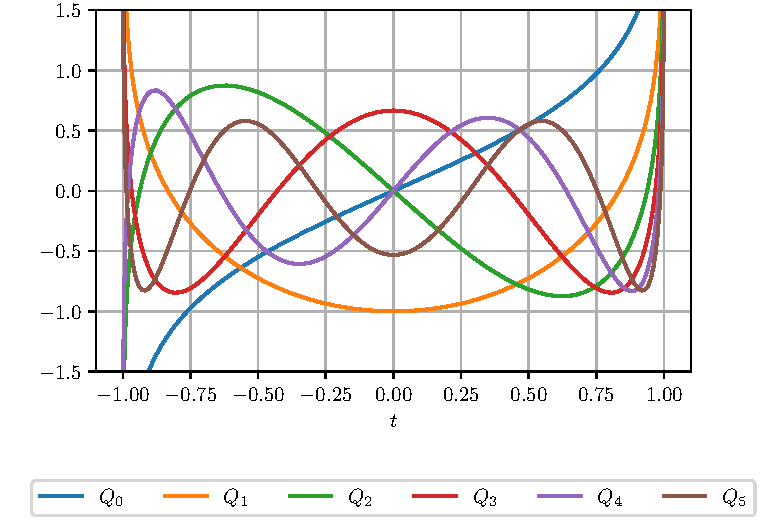
\includegraphics{./fig-legendre-polynomials-qn.pdf}
\caption{Legendreove polynómy druhého druhu reálneho argumentu $t$.}
\label{fig:lp_2nd}
\end{figure}

\begin{figure}
\centering
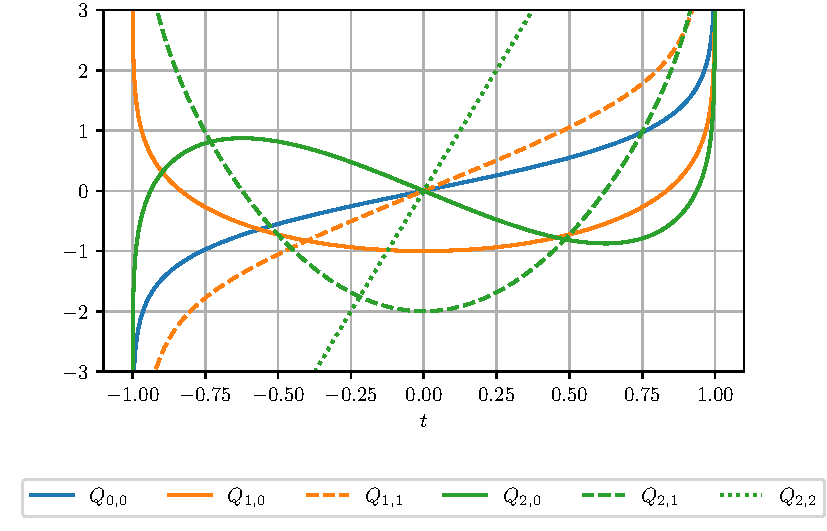
\includegraphics{./fig-legendre-functions-qnm.pdf}
\caption{Legendreove funkcie druhého druhu reálneho argumentu $t$.}
\label{fig:lf_2nd}
\end{figure}

Rovnica~(\ref{eq:qnm_real_def}) je formálne podobná rovnici~(\ref{eq:pnm_def}).  
Napriek tomu, v~dôsledku rozdielnej definície derivovaných členov~$Q_n(t)$ ide 
o~funkcie s~odlišným priebehom v~porovnaní s~$P_{nm}(t)$.  Uveďme pre názornosť 
explicitný vzťah na výpočet~$Q_0\left( t \right)$, $Q_1\left( t \right)$ 
a~$Q_2\left( t \right)$ pre reálny argument~$t$ a porovnajme tieto vzťahy 
s~rovnicami~(\ref{eq:p0_to_p5})
\parencite{MoritzPhysicalGeodesy},
%
\begin{equation}
\label{eq:q0t}
Q_0(t) = \frac{1}{2} \, \ln\frac{1 + t}{1 - t} = \mathrm{arctanh}(t){,}
\end{equation}
%
\begin{equation}
\label{eq:q1t}
Q_1(t) = \frac{t}{2} \, \ln\frac{1 + t}{1 - t} - 1 = t \, \mathrm{arctanh}(t)- 
 1{,}
\end{equation}
%
\begin{equation}
\label{eq:q2t}
Q_2(t) = \left( \frac{3}{4} t^2 - \frac{1}{4} \right) \, \ln\frac{1 + t}{1 - t} 
- \frac{3}{2}t = \left( \frac{3}{2} t^2 - \frac{1}{2} \right) \, 
\mathrm{arctanh}(t) - \frac{3}{2}t{,}
\end{equation}
%
kde
%
\begin{equation}
\label{eq:tanh}
\frac{1}{2} \, \ln \frac{1 + t}{1 - t} = \mathrm{arctanh} \, t{,}
\end{equation}
%
pričom $\mathrm{arctanh}$ označuje inverznú funkciu k~hyperbolickému tangensu, 
ktorý je daný vzťahom \parencite{Gradshteyn2007}
%
\begin{equation}
\tanh t = \frac{e^t - e^{-t}}{e^t + e^{-t}}{.}
\end{equation}
%
Funkcie $Q_{nm}(t)$ pre niekoľko prvých stupňov~$n$ a~rádov~$m$ sú znázornené 
na Obrázkoch~\ref{fig:lp_2nd} a~\ref{fig:lf_2nd} (porovnaj 
s Obrázkami~\ref{fig:lp} a~\ref{fig:lf}).  Funkcie $Q_0\left( z \right)$, 
$Q_1\left( z \right)$ a~$Q_2\left( z \right)$ komplexného argumentu~$z$ získame 
nahradením~výrazu~(\ref{eq:tanh}) vo vzťahoch~(\ref{eq:q0t}) až (\ref{eq:q2t}) 
výrazom (porovnaj rovnice~\ref{eq:qn0_imag_def} a~\ref{eq:qn0_real_def})
%
\begin{equation}
\label{eq:arccoth}
\frac{1}{2} \, \ln \frac{z + 1}{z - 1} = \mathrm{arccoth} \, z{,}
\end{equation}
%
kde $\mathrm{arccoth}$ je inverzná funkcia k hyperbolickému kotangensu, ktorý 
je daný vzťahom \parencite{Gradshteyn2007}
%
\begin{equation}
\coth z = \frac{1}{\tanh z} =  \frac{e^z + e^{-z}}{e^z - e^{-z}}{.}
\end{equation}

Pre~$Q_n(t)$ platia rovnaké rekurentné vzťahy ako pre~$P_n(t)$ 
\parencite{MoritzPhysicalGeodesy}.  Podobne ako funkcie $P_{nm}(t)$, i~funkcie 
$Q_{nm}(t)$ vyhovujú Legendreovej diferenciálnej rovnici druhého rádu 
\parencite[pozri rovnicu
\ref{eq:legfunc1_differential_equation};][]{MoritzPhysicalGeodesy}.  Všimnime 
si tiež, že Legendreove funkcie druhého druhu nadobúdajú hodnotu $\pm \infty$ 
pre $t \rightarrow \pm 1$, teda pre $\beta \rightarrow \pm \frac{\pi}{2}$ 
(pozri rovnice~\ref{eq:qn0_imag_def} a~\ref{eq:qn0_real_def} 
a Obrázky~\ref{fig:lp_2nd} a~\ref{fig:lf_2nd}).  Túto vlastnosť budeme nazývať 
\emph{singularita}.  Práve kvôli singularite sa Legendreove funkcie druhého 
druhu nepoužívajú v~praktických aplikáciách ako riešenie pre funkcie 
$g_\mathrm{s}(\varphi)$ a $g_\mathrm{r}(\beta)$ (pozri rovnice~\ref{eq:gs} 
a~\ref{eq:gr}), a to napriek tomu, že sú taktiež riešením Legendreovej 
diferenciálnej rovnice \parencite{MoritzPhysicalGeodesy}.


\subsection{Numerický výpočet Legendreových funkcií druhého druhu}

Presný a~efektívny numerický výpočet funkcií $Q_{nm}\left( i \frac{u}{E} 
\right)$, obzvlášť pre vysoké stupne a rády, je netriviálna úloha, podobne ako 
v~prípade funkcií $P_{nm}(t)$.  Z~dôvodov, ktoré budú ozrejmené 
v~Kapitole~\ref{sec:spheroidal_harmonic_expansion} sa v~praktických 
geodetických aplikáciách nezvyknú počítať členy $Q_{nm}\left( i \frac{u}{E} 
\right)$, ale podiely Legendreových funkcií $Q_{nm}\left( i \frac{u}{E} \right) 
\slash Q_{nm}\left( i \frac{b}{E} \right)$.  Samotný výpočet, či už funkcií 
$Q_{nm}\left( i \frac{u}{E} \right)$ alebo $Q_{nm}\left( i \frac{u}{E} \right) 
\slash Q_{nm}\left( i \frac{b}{E} \right)$, je zvyčajne uskutočňovaný 
rekurentnými vzťahmi alebo rozvojmi do nekonečných radov \parencite[pozri 
napríklad][]{Sebera2012,Fukushima2013,Wang2013,Sprlak2020}.



\section{Rozvoj gravitačného potenciálu do radu sféroidických harmonických 
funkcií}
\label{sec:spheroidal_harmonic_expansion}

Gravitačný potenciál mimo hmôt telesa môže byť rozvinutý do radu sféroidických 
harmonických funkcií vzťahom
%
\begin{equation}
\label{eq:vg_spheroidalh_2nd_norm_ynk}
V_\gidx(u, \beta, \lambda) = \frac{GM}{R} \, \sum_{n = 0}^\infty \sum_{k 
= -n}^n \frac{Q_{n|k|}\left( i \dfrac{u}{E} \right)}{Q_{n|k|}\left( 
i \dfrac{b}{E} \right)} \, \bar{v}^{\mathrm{r}}_{nk} \, \bar{Y}_{nm}(\beta, 
\lambda){,}
\end{equation}
%
kde $\bar{v}_{nk}^\mathrm{r}$ sú \emph{úplne normované sféroidické harmonické 
koeficienty} gravitačného potenciálu.  
Rovnica~(\ref{eq:vg_spheroidalh_2nd_norm_ynk}) je formálne podobná 
vzťahu~(\ref{eq:vg_sh_2nd_norm_ynk}).  Môže byť tiež jednoducho prepísaná do 
tvaru, ktorý využíva index~$m = 0, 1, \dots, n$ (porovnaj 
rovnice~\ref{eq:vg_sh_2nd_norm} a~\ref{eq:vg_sh_2nd_norm_ynk}) či do radu 
nenormovaných sféroidických harmonických funkcií, podobne ako je tomu 
v~rovniciach~(\ref{eq:vg_sh_no_norm}) a~(\ref{eq:vg_sh_1st_norm}),
%
\begin{equation}
\label{eq:vg_spheroidalh_no_norm}
V_\gidx(u, \beta, \lambda) = \sum_{n = 0}^\infty \sum_{m = 0}^n 
\frac{Q_{nm}\left( i \dfrac{u}{E} \right)}{Q_{nm}\left( i \dfrac{b}{E} \right)} 
\, \left( C^{\mathrm{r}}_{nm} \, \cos(m\lambda) + S^{\mathrm{r}}_{nm} \, 
\sin(m\lambda) \right) \, P_{nm}(\sin\beta){.}
\end{equation}
%
Funkcia $Q_{n|k|}\left( i \frac{u}{E} \right)$ zo vzťahu~(\ref{eq:gr}) je 
komplexná funkcia.  Vo sféroidických harmonických 
rozvojoch~(\ref{eq:vg_spheroidalh_2nd_norm_ynk}) 
a~(\ref{eq:vg_spheroidalh_no_norm}) je preto vydelená funkciou $Q_{n|k|}\left( 
i \frac{b}{E} \right)$ tak, aby výsledný podiel bol reálne číslo.  Tým je 
zabezpečené, že i~sféroidické harmonické koeficienty sú reálne čísla.  Všimnime 
si tiež, že pred prvou sumáciou vo vzťahu~(\ref{eq:vg_spheroidalh_no_norm}) sa 
nenachádza Newtonova gravitačná konštanta~$G$ tak, ako je tomu vo 
vzťahu~(\ref{eq:vg_sh_no_norm}).  Ide len konvenciu, konštanta $G$ je tým pádom 
obsiahnutá vo sféroidických harmonických koeficientoch $C_{nm}^\mathrm{r}$ 
a~$S_{nm}^\mathrm{r}$.

Člen $Q_{n|k|}\left( i \frac{u}{E} \right) \slash Q_{n|k|}\left( i \frac{b}{E} 
\right)$ v~rovnici~(\ref{eq:vg_spheroidalh_2nd_norm_ynk}) má podobnú úlohu, akú 
má člen $\left( \frac{R}{r} \right)^{n + 1}$ 
vo~vzťahu~(\ref{eq:vg_sh_2nd_norm_ynk}), teda umožniť výpočet gravitačného 
potenciálu aj nad referenčným elipsoidom (v~prípade sférického harmonického 
rozvoja nad referenčnou sférou s~polomerom~$R$).  V~súvislosti 
s~rovnicou~(\ref{eq:ellred2cart}) sme uviedli, že pre~$E = 0$ sú redukované 
elipsoidické súradnice $u$, $\beta$ a $\lambda$ totožné so sférickými 
súradnicami $r$, $\varphi$ a $\lambda$.  Pre $E \rightarrow 0$ tiež platí vzťah 
\parencite{MoritzPhysicalGeodesy}
%
\begin{equation}
\lim_{E \rightarrow 0} \frac{Q_{n|k|}\left( i \dfrac{u}{E} 
\right)}{Q_{n|k|}\left( i \dfrac{b}{E} \right)} = \left( \frac{R}{r} \right)^{n 
+ 1}{.}
\end{equation}
%
Sférický harmonický rozvoj~(\ref{eq:vg_sh_2nd_norm_ynk}) teda možno považovať 
za špeciálny prípad zovšeobecneného sféroidické harmonického 
rozvoja~(\ref{eq:vg_spheroidalh_2nd_norm_ynk}).

Na záver dodajme, že Laplaceovu rovnicu možno riešiť aj v~súradnicovom systéme, 
ktorý je vztiahnutý k~trojosovému elipsoidu s~polosami $a$, $b$ a $c$.  Získame 
tým rozvoj gravitačného potenciálu do radu elipsoidických harmonických funkcií 
\parencite[napríklad][]{Garmier2001,Hu2015,Reimond2016}.  Tento prístup je 
zložitejší ako sférické a~sféroidické harmonické rozvoje a vo fyzikálnej 
geodézii sa používa zriedka.  Využite má najmä v~súvislosti s~modelovaním 
gravitačného poľa asteroidov komplikovaných tvarov, pre ktoré nie je dostatočne 
presné používať sféru ani dvojosový rotačný elipsoid ako referenčné plochy.








% -----------------------------------------------------------------------------


\chapter{Normálne tiažové pole}
\label{sec:normal_gravity_field}

Fyzikálna geodézia určuje tvar Zeme z~informácie o~jej tiažovom poli, napríklad 
z~tiažového potenciálu a z~vektora tiažového zrýchlenia na povrchu Zeme.  Táto 
úloha je neľahká, pretože vzťah medzi tiažovým poľom a hľadaným zemským 
povrchom je nelineárny.  Spravidla sa preto pristupuje k~linearizácii rozvojom 
do Taylorovho radu, pričom členy druhého a vyšších rádov sa zanedbajú.  
\emph{Normálne tiažové pole Zeme} je jednoduchý a súčasne dostatočne presný 
model skutočného tiažového poľa Zeme, využívaný práve na výpočet približných 
hodnôt v linearizovaných úlohách fyzikálnej geodézie.  Požiadavka jednoduchosti 
je odôvodnená potrebou prijateľne náročných výpočtov v normálnom poli, 
napríklad pomocou uzavretých vzťahov pre \emph{normálne tiažové zrýchlenie} 
$\boldsymbol{\gamma}$ či \emph{normálny tiažový potenciál} $U$.  Dostatočná 
presnosť je potrebná nato, aby bolo možné s rozumnou mierou aproximácie 
zanedbať nelineárne členy Taylorovho rozvoja.  Požiadavky jednoduchosti 
a presnosti normálneho tiažového poľa si vzájomne odporujú, preto je potrebné 
nájsť medzi nimi vhodný kompromis.

\section{Voľba normálneho tiažového poľa}

Jedno z najjednoduchších telies ponúkajúcich sa na definíciu normálneho 
tiažového poľa Zeme je \emph{homogénna rotujúca guľa} definovaná nezávislými 
parametrami $GM$, $R$ a $\omega$, teda geocentrickou gravitačnou konštantou, 
polomerom gule a uhlovou rýchlosťou rotácie.  Vonkajšie tiažové pole homogénnej 
gule je síce jednoducho matematicky opísateľné, nevyhovuje však väčšine 
súčasných aplikácií z hľadiska presnosti.  Vo fyzikálnej geodézii sa zvykne 
preto využívať prevažne len v~niektorých špecifických situáciách, napríklad ak 
postačuje i~nižšia presnosť.

V dôsledku sploštenia Zeme je dvojosový rotačný elipsoid presnejšou 
geometrickou aproximáciou geoidu ako sféra.  Okrem svojho geometrického tvaru 
je geoid špecifický tým, že hodnota skutočného tiažového potenciálu $W_0$ je 
konštantná v~každom jeho bode (pozri Kapitolu~\ref{sec:equipotential_surface}).  
Túto vlastnosť by bolo výhodné zužitkovať aj pri voľbe normálneho tiažového 
poľa.  Budeme preto požadovať, aby \emph{normálny tiažový potenciál} $U_0$ bol 
na povrchu elipsoidu konštantný.  Vhodnou voľbou geometrických parametrov 
(napríklad hlavná a vedľajšia polos) a fyzikálnych parametrov (napríklad 
normálny tiažový potenciál $U_0$) potom získame vernú aproximáciu geoidu, alebo 
inými slovami, dostatočne presné približné hodnoty na linearizáciu úloh 
spojených s určovaním geoidu.  Dvojosový rotačný elipsoid s~konštantným 
normálnym tiažovým potenciálom na svojom povrchu sa nazýva 
\emph{ekvipotenciálny elipsoid}.  V~súčasnosti je to najčastejší spôsob voľby 
normálneho tiažového poľa Zeme.

Ďalšou možnosťou voľby normálneho tiažového poľa je sférický harmonický rozvoj 
gravitačného potenciálu do konečného harmonického stupňa 
(rovnice~\ref{eq:vg_sh_no_norm}, \ref{eq:vg_sh_1st_norm}, 
\ref{eq:vg_sh_2nd_norm} a \ref{eq:vg_sh_2nd_norm_ynk}).  Plocha, na ktorej je 
takto definovaný normálny tiažový potenciál konštantný sa nazýva 
\emph{sféroid}.  Obmedzením rozvoja potenciálu na stupeň~2 získame 
\emph{Brunsov sféroid} a obmedzením na stupeň~4 získame \emph{Helmertov 
sféroid} \parencite{Moritz1967}.  V~oboch prípadoch sú koeficienty stupňa~1 
nulové, pretože začiatok súradnicového systému je vložený do ťažiska Zeme 
(pozri~Kapitolu~\ref{sec:physical_meaning_of_spherical_harmonic_coefficients}).  
V definícii Helmertovho sféroidu sú nulové navyše aj koeficienty stupňa~3 
z dôvodu zabezpečenia symetrie voči rovine rovníka (pozri geometrickú 
interpretáciu sférických harmonických funkcií 
v~Kapitole~\ref{sec:spherical_harmonics}).  V súčasnosti sa Brunsov ani 
Helmertov sféroid nezvyknú používať v praktických aplikáciách.  Obe plochy sú 
totiž veľmi blízke dvojosovému rotačnému elipsoidu, no sú výrazne zložitejšie.  
Navyše, získaná dodatočná presnosť zväčša nie je významná 
\parencite{Moritz1967}.

Či už ide o homogénnu rotujúcu guľu, ekvipotenciálny elipsoid alebo sféroid, 
všimnime si, že v~ani jednom prípade sme nepotrebovali vysloviť predpoklad 
o~priestorovom rozložení hustôt vo vnútri týchto telies.  Fyzikálna geodézia 
využíva normálne tiažové pole predovšetkým na účely linearizácie.  Zdá sa byť 
preto kľúčové najmä to, aby normálna ekvipotenciálna plocha s~normálnym 
tiažovým potenciálom~$U_0$ bola geometricky blízka geoidu, ďalej aby normálny 
tiažový potenciál~$U_0$ bol blízky skutočnému tiažovému potenciálu~$W_0$ na 
geoide, a nakoniec aby geometrická aj fyzikálna časť normálneho poľa boli 
jednoducho matematicky popísateľné.  Pre niektoré príbuzné vedné odbory, 
napríklad geofyziku, je však znalosť hustoty v~normálnom telese potrebná 
\parencite{Karcol2017}.  Zdá sa, že v~takýchto situáciách nie je voľba 
ekvipotenciálneho elipsoidu najvýhodnejšia.  Diskusiu k~možnostiam 
priestorového rozloženia hustoty vo vnútri ekvipotenciálneho elipsoidu je možné 
nájsť napríklad v~prácach \textcite{MoritzTheFigureOfTheEarth}, 
\textcite{TorgeGeodesy}, \textcite{Conway2000} či \textcite{Karcol2017}.



\section{Ekvipotenciálny elipsoid}
\label{sec:equipotential_ellipsoid}

Nech teleso s~hmotnosťou~$M$ rotuje konštantnou uhlovou rýchlosťou~$\omega$ 
okolo pevnej osi.  Nech $S$ je ekvipotenciálna plocha jeho tiažového poľa 
obklopujúca celé teleso.  \emph{Stokesov--Poincarého} teorém hovorí, že tiažový 
potenciál vo vonkajšom priestore plochy~$S$ je jednoznačne určený konštantami 
$M$ a $\omega$ a parametrami definujúcimi plochu~$S$ \parencite{TorgeGeodesy}.

Na jednoznačné zadefinovanie ekvipotenciálneho elipsoidu a jeho vonkajšieho 
tiažového poľa preto postačuje určiť štyri nezávislé \emph{základné parametre}.  
Dva z týchto parametrov sú geometrické, resp. veľmi úzko súvisia s geometriou 
elipsoidu (napríklad hlavná polos a sploštenie elipsoidu), a dva parametre sú 
fyzikálne (hmotnosť a uhlová rýchlosť rotácie).  Všetky ostatné veličiny 
normálneho tiažového poľa je možné vypočítať z~týchto základných parametrov, či 
už ide o geometrické parametre (napríklad vedľajšia polos či lineárna 
excentricita elipsoidu) alebo fyzikálne parametre (normálny tiažový potenciál 
a pod.).  Parametre, ktoré sú vypočítané zo základných parametrov budeme 
nazývať \emph{odvodené parametre}.  Teóriu ekvipotenciálneho elipsoidu 
rozpracovali taliansky geodet, astronóm, geofyzik a matematik P.~Pizzetti 
(1860--1918) a~taliansky matematik a matematický fyzik C.~Somigliana 
(1860--1955) v~prácach \textcite{Pizzetti1984} a \textcite{Somigliana1929}.

Základné parametre ekvipotenciálnych elipsoidov sú v súčasnosti určované 
spravidla družicovými technikami a astronomickými meraniami.  Historický 
prehľad geodetických referenčných systémov a spôsoby ich určenia je možné nájsť 
napríklad v~prácach \textcite{TorgeGeodesy} a~\textcite{MoritzPhysicalGeodesy}.  
V ďalších častiach práce popíšeme dva najpoužívanejšie ekvipotenciálne 
elipsoidy (Kapitoly~\ref{sec:grs80} a \ref{sec:wgs84}).  Následne odvodíme 
vzťahy na výpočet normálneho tiažového potenciálu pomocou rozvoja do radu 
sféroidických a sférických harmonických 
funkcií~(Kapitola~\ref{sec:normal_gravity_potential}).  Na záver opíšeme spôsob 
výpočtu normálneho tiažového zrýchlenia (Kapitola~\ref{sec:normal_gravity}).  
Tieto poznatky budú dôležité neskôr v~Kapitole~\ref{sec:geoid_determination}, 
ktorá sa zaoberá určovaním geoidu.  Dodajme, že hoci budeme často hovoriť 
o~normálnom tiažovom poli \emph{Zeme}, je dobré mať na pamäti, že ide 
o~matematicko-fyzikálny model definovaný štyrmi základnými parametrami.  Všetky 
ostatné parametre, či už geometrické alebo fyzikálne, sú odvoditeľné z~týchto 
parametrov.  S~výnimkou štyroch základných parametrov sa teda všetky veličiny 
normálneho tiažového poľa získavajú výpočtom, nie meraním ako je tomu v prípade 
\emph{skutočného} tiažového poľa Zeme.





\subsection{Ekvipotenciálny elipsoid GRS80}
\label{sec:grs80}

Jednu z možných štvoríc základných parametrov tvorí
%
\begin{itemize}
\item hlavná polos~$a$,
%
\item dynamický koeficient~$J_{2,0}$,
%
\item geocentrická gravitačná konštanta~$GM$ a
%
\item uhlová rýchlosť rotácie $\omega$.
\end{itemize}
%
Týmto základnými parametrami je definovaný ekvipotenciálny elipsoid 
\emph{GRS80} \parencite[angl. \textit{Geodetic Reference 
System~1980};][]{GRS80}.  Základné parametre GRS80 (Tabuľka~\ref{tab:1}) boli 
prijaté Medzinárodnou úniou geodézie a geofyziky (angl. \textit{International 
Union of Geodesy and Geophysics}, IUGG) a Medzinárodnou asociáciou geodézie IAG 
na 17.~generálnom zasadnutí IUGG v Canberra v decembri 1979.  Dôležité je 
spomenúť, že použitá hodnota konštanty $GM$ zahŕňa hmotnosť Zeme \emph{a} 
hmotnosť zemskej atmosféry a koeficient $J_{2,0}$ nezahŕňa účinok permanentnej 
slapovej deformácie Zeme.  Medzi koeficientmi $J_{2,0}$ (Tabuľka~\ref{tab:1}), 
$C_{2,0}$ (rovnica~\ref{eq:vg_sh_no_norm}) a $\bar{C}_{2,0}$ 
(rovnica~\ref{eq:vg_sh_2nd_norm}) platia nasledovné vzťahy 
\parencite{Moritz1967,MoritzPhysicalGeodesy},
%
\begin{equation}
C_{2,0} = -J_{2,0}{,}
\end{equation}
%
\begin{equation}
\bar{C}_{2,0} = \frac{C_{2,0}}{\sqrt{5}} = -\frac{J_{2,0}}{\sqrt{5}}{.}
\end{equation}
%
Niektoré odvodené parametre sú uvedené v~Tabuľke~\ref{tab:2}.  Elipsoid GRS80 
je oficiálny referenčný systém Medzinárodnej asociácie geodézie.

\begin{table*}
\begin{center}
\caption{Základné parametre ekvipotenciálneho elipsoidu GRS80}
\label{tab:1}
\small
\begin{tabular}{l l l l}
\hline
Označenie & Symbol & Jednotka & Popis\\
\hline
$a$       & $6\,378\,137$ & m & Hlavná polos\\
$J_{2,0}$ & $108\,263 \times 10^{-8}$ & Bezrozmerné & Dynamický faktor\\
$GM$ & $3\,986\,005 \times 10^8$ & $\mathrm{m}^3 \ \mathrm{s}^{-2}$ 
& Geocentrická gravitačná konštanta\\
$\omega$ & $7\,292\,115 \times 10^{-11}$ & $\mathrm{rad} \ \mathrm{s}^{-1}$ 
& Uhlová rýchlosť rotácie\\
\hline
\end{tabular}
\end{center}
\end{table*}

\begin{table*}
\begin{center}
\caption{Niektoré odvodené parametre ekvipotenciálneho elipsoidu GRS80 
\parencite{MoritzPhysicalGeodesy}}
\label{tab:2}
\small
\begin{tabular}{l l l l l}
\hline
Typ parametra & Symbol & Hodnota & Jednotka & Popis\\
\hline
Geometrický & $b$       & $6 \, 356 \, 752.3141$ & m & Vedľajšia polos\\
            & $E$       & $521 \, 854.0097$ & m & Lineárna excentricita\\
            & $e^2$     & $0.00669438002290$ & Bezrozmerné & Druhá mocnina 
            prvej\\
            &           &     &             & numerickej excentricity\\
            & $(e')^2$  & $0.00673949677548$ & Bezrozmerné & Druhá mocnina 
            druhej\\
            &           &     &             & numerickej excentricity\\
            & $f$       & $0.00335281068118$ & Bezrozmerné & Sploštenie\\
\hline
Fyzikálny & $U_0$       & $ 62 \, 636 \, 860.850$ & $\mathrm{m}^2 \, 
          \mathrm{s}^{-2}$ & Normálny tiažový\\
          &            &     &   & potenciál na elipsoide\\
          & $\gamma_a$ & $9.7803267715$ & $\mathrm{m} \, \mathrm{s}^{-2}$ 
& Normálne tiažové\\
          &            &     &   & zrýchlenie na rovníku\\
          & $\gamma_b$ & $9.8321863685$ & $\mathrm{m} \, \mathrm{s}^{-2}$ 
& Normálne tiažové\\
          &            &     &   & zrýchlenie na póle\\
          & $m$ & $0.00344978600308$ & Bezrozmerné & $m = \omega^2 \, a^2 \, 
b \slash (GM)$\\
\hline
\end{tabular}
\end{center}
\end{table*}






\subsection{Ekvipotenciálny elipsoid WGS84}
\label{sec:wgs84}

Ďalšou možnosťou definície ekvipotenciálneho elipsoidu je použiť sploštenie~$f$ 
namiesto koeficientu~$J_{2,0}$,
%
\begin{equation}
f = \frac{a - b}{b}{.}
\end{equation}
%
Týmto spôsobom je definovaný ekvipotenciálny elipsoid \emph{WGS4} 
\parencite[angl. \textit{World Geodetic System~1984};][]{WGS84}, ktorý vychádza 
z~elipsoidu GRS80 (Tabuľka~\ref{tab:3}).  Vybraté odvodené parametre elipsoidu 
WGS84 sú uvedené v~Tabuľke~\ref{tab:4}.  Z hľadiska tvaru sú oba elipsoidy 
podobné; dĺžka ich hlavnej polosi je $6\, 378\, 137\ \mathrm{m}$ a dĺžka 
vedľajšej polosi, vypočítaná zo základných parametrov, sa odlišuje iba 
o~desatinu milimetra (porovnaj Tabuľky~\ref{tab:2} a~\ref{tab:4}).  
Z fyzikálneho hľadiska je už medzi elipsoidmi rozdiel väčší.  Uhlová rýchlosť 
rotácie oboch elipsoidov je síce rovnaká, no odlišné hodnoty geocentrických 
gravitačných konštánt spôsobujú rozdiel v~normálnom tiažovom potenciáli na 
elipsoide.  Rozdiel medzi oboma hodnotami je približne o~5 rádov väčší ako 
presnosť určenia rozdielu skutočného tiažového potenciálu medzi dvoma bodmi 
(pozri Kapitolu~\ref{sec:centrifugal_and_gravity_potential}).

\begin{table*}
\begin{center}
\caption{Základné parametre ekvipotenciálneho elipsoidu WGS84}
\label{tab:3}
\small
\begin{tabular}{l l l l}
\hline
Označenie & Symbol & Jednotka & Popis\\
\hline
$a$       & $6\,378\,137$ & m & Hlavná polos\\
$1 \slash f$ & $298.257223563$ & Bezrozmerné & Prevrátená hodnota sploštenia\\
$GM$ & $3\,986\,004.418 \times 10^8$ & $\mathrm{m}^3 \ \mathrm{s}^{-2}$ 
& Geocentrická gravitačná konštanta\\
$\omega$ & $7\,292\,115 \times 10^{-11}$ & $\mathrm{rad} \ \mathrm{s}^{-1}$ 
& Uhlová rýchlosť rotácie\\
\hline
\end{tabular}
\end{center}
\end{table*}

\begin{table*}
\begin{center}
\caption{Niektoré odvodené parametre ekvipotenciálneho elipsoidu WGS84 
\parencite{MoritzPhysicalGeodesy}}
\label{tab:4}
\small
\begin{tabular}{l l l l l}
\hline
Typ parametra & Symbol & Hodnota & Jednotka & Popis\\
\hline
Geometrický & $b$       & $6 \, 356 \, 752.3142$ & m & Vedľajšia polos\\
            & $E$       & $521 \, 854.0084$ & m & Lineárna excentricita\\
            & $e^2$     & $0.00669437999014$ & Bezrozmerné & Druhá mocnina 
            prvej\\
            &           &     &             & numerickej excentricity\\
            & $(e')^2$  & $0.00673949674228$ & Bezrozmerné & Druhá mocnina 
            druhej\\
            &           &     &             & numerickej excentricity\\
            & $J_{2,0}$       & $108262.982131 \times 10^{-8}$ & Bezrozmerné 
& Dynamický faktor\\
\hline
Fyzikálny & $U_0$       & $ 62 \, 636 \, 851.715$ & $\mathrm{m}^2 \, 
          \mathrm{s}^{-2}$ & Normálny tiažový\\
          &            &     &   & potenciál na elipsoide\\
          & $\gamma_a$ & $9.7803253359$ & $\mathrm{m} \, \mathrm{s}^{-2}$ 
& Normálne tiažové\\
          &            &     &   & zrýchlenie na rovníku\\
          & $\gamma_b$ & $9.8321849378$ & $\mathrm{m} \, \mathrm{s}^{-2}$ 
& Normálne tiažové\\
          &            &     &   & zrýchlenie na póle\\
          & $m$ & $0.00344978650684$ & Bezrozmerné & $m = \omega^2 \, a^2 \, 
b \slash (GM)$\\
\hline
\end{tabular}
\end{center}
\end{table*}






\section{Normálny tiažový potenciál}
\label{sec:normal_gravity_potential}

V~mnohých situáciách, hoci rozhodne nie v~každej situácii, sú 
preferované~uzavreté matematické vzťahy pred nekonečnými rozvojmi.  Uzavretý 
vzťah je taký vzťah, ktorý má konečný počet členov.  Jeho výhodou je, že často 
umožňuje presnejší a rýchlejší číselný výpočet v~porovnaní s~výpočtom 
nekonečného radu.  V praktických výpočtoch musí byť nekonečný rad vždy 
obmedzený na vhodne zvolený konečný počet členov.  
V~Kapitole~\ref{sec:normal_gravity_potential_in_reduced_ell_coords} sa preto 
budeme snažiť nájsť uzavretý vzťah na výpočet normálneho tiažového 
potenciálu~$U$ v~bodoch na povrchu ekvipotenciálneho elipsoidu a~nad ním.  Za 
týmto účelom budeme pracovať v~redukovaných elipsoidických súradniciach, ktoré 
sa prirodzene ponúkajú v~súvislosti so splošteným rotačným elipsoidom.  
Následne v~Kapitole~\ref{sec:normal_gravity_potential_in_spherical_coords} 
vyjadríme normálny tiažový potenciál vo sférických súradniciach, tentokrát však 
už pomocou nekonečného rozvoja.  
Kapitola~\ref{sec:normal_gravity_potential_in_reduced_ell_coords} je spracovaná 
podľa~\textcite{MoritzTheFigureOfTheEarth}.

\subsection{Normálny tiažový potenciál vyjadrený v~elipsoidických redukovaných 
súradniciach}
\label{sec:normal_gravity_potential_in_reduced_ell_coords}

Vzťah~(\ref{eq:vg_spheroidalh_no_norm}) popisuje vonkajší gravitačný potenciál 
všeobecného telesa.  Ak k nemu pripočítame odstredivý potenciál vyjadrený 
v~redukovaných elipsoidických súradniciach (pozri rovnice~\ref{eq:vc} 
a~\ref{eq:ellred2cart}),
%
\begin{equation}
\label{eq:vc_spheroidal}
V_\cidx = \frac{1}{2} \, \omega^2 \, (u^2 + E^2) \, \cos^2\beta{,}
\end{equation}
%
získame vzťah pre tiažový potenciál $W$ všeobecného telesa (pozri 
rovnicu~\ref{eq:w}).  Normálny tiažový potenciál~$U$ ekvipotenciálneho 
elipsoidu je však opísateľný jednoduchším spôsobom ako tiažový potenciál 
\emph{všeobecného} telesa, pretože má dve symetrie, jednu voči osi rotácie 
a druhú voči rovine rovníka.  Prvá symetria spôsobuje, že všetky nezonálne 
sféroidické harmonické koeficienty musia byť nulové, pretože tieto členy 
závisia od dĺžky~$\lambda$ (pozri rovnicu~\ref{eq:vg_spheroidalh_no_norm}).  
Druhá symetria spôsobuje, že nenulové môžu byť iba párne zonálne koeficienty 
(pozri vlastnosti sférických harmonických funkcií 
Kapitolu~\ref{sec:spherical_harmonics}).  Normálny tiažový potenciál môžeme 
teda zapísať v~tvare
%
\begin{equation}
\label{eq:u_sph}
\begin{split}
U(u, \beta) &= U_\gidx(u, \beta) + U_\cidx(u, \beta)\\
%
&=\sum_{n = 0}^\infty \frac{Q_n\left( i \dfrac{u}{E} \right)}{Q_n\left( 
i \dfrac{b}{E} \right)} \,  C^{\mathrm{r}}_n \, P_n(\sin\beta) + \frac{1}{2} \, 
\omega^2 \, (u^2 + E^2) \, \cos^2\beta{,}
\end{split}
\end{equation}
%
kde $U_\gidx$ je normálny gravitačný potenciál 
(rovnica~\ref{eq:vg_spheroidalh_no_norm}) a $U_\cidx$ je normálny odstredivý 
potenciál (rovnica~\ref{eq:vc_spheroidal}).  Pre lepšiu názornosť nasledujúcich 
krokov sme do vzťahu~(\ref{eq:u_sph}) zahrnuli aj nepárne zonálne 
koeficienty~$C^{\mathrm{r}}_n$ hoci sú nulové.

Z Kapitoly~\ref{sec:spherical_harmonic_expansion} vieme, že ak chceme poznať 
$U(u,\beta)$ z~rovnice~(\ref{eq:u_sph}), potom potrebujeme poznať 
koeficienty~$C_n^\mathrm{r}$.  Zatiaľ čo v~prípade skutočného poľa Zeme je 
potrebné koeficienty~$C_{nm}$ a~$S_{nm}$ (pozri rovnicu~\ref{eq:vg_sh_no_norm}) 
vypočítať z~meraní skutočného poľa 
(Kapitola~\ref{sec:spherical_harmonics_applications}), koeficienty normálneho 
poľa $C_n^\mathrm{r}$ je možné vypočítať zo štyroch základných parametrov 
ekvipotenciálneho elipsoidu (pozri Kapitolu~\ref{sec:equipotential_ellipsoid}).  
Skúsme preto zistiť, čomu sú rovné sféroidické harmonické koeficienty 
$C_n^\mathrm{r}$.

Nech sa výpočtový bod nachádza na povrchu ekvipotenciálneho elipsoidu, teda $u 
= b$.  Potom
%
\begin{equation}
\frac{Q_n\left( i \dfrac{u}{E} \right)}{Q_n\left( i \dfrac{b}{E} \right)} 
= 1{,} \quad u = b{,}
\end{equation}
%
a rovnica~(\ref{eq:u_sph}) prejde do tvaru
%
\begin{equation}
\label{eq:u_sph_on_ell}
U(b, \beta) = \sum_{n = 0}^\infty C^{\mathrm{r}}_n \, P_n(\sin\beta) 
+ \frac{1}{2} \, \omega^2 \, (b^2 + E^2) \, \cos^2\beta = U_0{.}
\end{equation}
%
Hodnota~normálneho tiažového potenciálu na ekvipotenciálnom elipsoide $U_0$ je 
z definície konštantná (pozri Kapitolu~\ref{sec:equipotential_ellipsoid}).

Prostredná časť rovnice~(\ref{eq:u_sph_on_ell}) je formálne podobná 
vzťahu~(\ref{eq:f_synthesis}) avšak s~dvoma rozdielmi.  Po prvé, je rovná 
konštante $U_0$ a nie funkcii $f(t)$, ktorá by závisela od $t = \sin\beta$.  Po 
druhé, druhý člen v~prostrednej časti rovnice obsahuje člen $\cos^2\beta$, 
ktorý, podobne ako Legendreove polynómy, závisí od $\sin\beta$, pretože 
$\cos^2\beta = 1 - \sin^2\beta$.  Prepíšme preto 
rovnicu~(\ref{eq:u_sph_on_ell}) do tvaru
%
\begin{equation}
\label{eq:cnr}
\sum_{n = 0}^\infty C^{\mathrm{r}}_n \, P_n(\sin\beta) + \frac{1}{3} \, 
\omega^2 \, a^2  - \frac{1}{3} \, \omega^2 \, a^2 \, P_2(\sin\beta) - U_0 
= 0{.}
\end{equation}
%
Na získanie tejto rovnice sme použili vzťah (pozri 
rovnicu~\ref{eq:linear_eccentricity})
%
\begin{equation}
a^2 = b^2 + E^2{,}
\end{equation}
%
a vzťah pre Legendreov polynóm stupňa $n = 2$ (rovnica~\ref{eq:p0_to_p5})
%
\begin{equation}
P_2(\sin\beta) = \frac{3}{2} \, \sin^2\beta - \frac{1}{2}{.}
\end{equation}

Keďže $P_0(\sin\beta) = 1$ (pozri rovnicu~\ref{eq:p0_to_p5}), 
vzťah~(\ref{eq:cnr}) môžeme ďalej prepísať do tvaru
%
\begin{equation}
\label{eq:cnr2}
\begin{split}
&\left( C_0^\mathrm{r} + \frac{1}{3} \, \omega^2 \, a^2 - U_0 \right) \, 
P_0(\sin\beta) + C_1^\mathrm{r} \, P_1(\sin\beta) + \left(C_2^\mathrm{r} 
- \frac{1}{3} \, \omega^2 \, a^2 \right) \, P_2(\sin\beta)\\
%
&+ \sum_{n = 3}^\infty C^{\mathrm{r}}_n \, P_n(\sin\beta) = 0{.}
\end{split}
\end{equation}
%
Tento vzťah predstavuje rozvoj podobný vzťahu~(\ref{eq:f_synthesis}), pričom 
členy pred jednotlivými Legendreovými polynómami sú súradnice konštantnej 
funkcie~0, ktorá sa nachádza na pravej strane rovnice (pozri diskusiu 
o~súradniciach ku vzťahom~\ref{eq:r_synthesis}, \ref{eq:f_synthesis} 
a \ref{eq:f_sha_no_norm}).  Podobne ako rovnosť (pozri 
vzťah~\ref{eq:r_synthesis})
%
\begin{equation}
\sum_{i = 1}^3 r_i \, \vec{e}_i = \vec{0}
\end{equation}
%
platí vtedy a iba vtedy, ak $r_i = 0$ pre všetky $i$, podobne aj 
vzťah~(\ref{eq:cnr2}) platí vtedy a iba vtedy, ak
%
\begin{equation}
\begin{split}
C_0^\mathrm{r} + \frac{1}{3} \, \omega^2 \, a^2 - U_0 &= 0{,}\\
C_1^\mathrm{r}                                        &= 0{,}\\
C_2^\mathrm{r} - \frac{1}{3} \, \omega^2 \, a^2       &= 0{,}\\
C_n^\mathrm{r}                                        &= 0 \quad \textrm{pre} 
\quad n \geq 3{.}
\end{split}
\end{equation}
%
Z toho ale vyplýva, že
%
\begin{equation}
\label{eq:cnr3}
\begin{split}
C_0^\mathrm{r} &= U_0 - \frac{1}{3} \, \omega^2 \, a^2{,}\\
C_1^\mathrm{r} &= 0{,}\\
C_2^\mathrm{r} &= \frac{1}{3} \, \omega^2 \, a^2{,}\\
C_n^\mathrm{r} &= 0 \quad \textrm{pre} \quad n \geq 3{.}
\end{split}
\end{equation}
%
Normálny gravitačný potenciál je teda po dosadení koeficientov~(\ref{eq:cnr3}) 
do rovnice~(\ref{eq:u_sph}) daný vzťahom
%
\begin{equation}
\label{eq:ug_spheroidal}
U_\gidx(u, \beta) = \left( U_0 - \frac{1}{3} \, \omega^2 \, a^2 \right) \, 
\frac{Q_0\left( i \dfrac{u}{E} \right)}{Q_0\left( i \dfrac{b}{E} \right)} 
+ \frac{1}{3} \, \omega^2 \, a^2  \, \frac{Q_2\left( i \dfrac{u}{E} 
\right)}{Q_2\left( i \dfrac{b}{E} \right)} \, P_2(\sin\beta){.}
\end{equation}
%
Všimnime si niektoré dôležité vlastnosti rovnice~(\ref{eq:ug_spheroidal}).  
Vzťahy pre~$Q_0(z)$ a $Q_2(z)$ komplexného argumentu $z$ sú konečné (pozri 
Kapitolu~\ref{sec:spheroidal_harmonics}).  Po dosadení~(\ref{eq:ug_spheroidal}) 
do~(\ref{eq:u_sph}) preto získame vzťah pre normálny tiažový potenciál, ktorý 
má konečný počet členov, čo bol cieľ vytýčený na začiatku tejto kapitoly.  
Ďalšia dôležitá vlastnosť je tá, že vzťah~(\ref{eq:ug_spheroidal}) platí nielen 
na elipsoide pre $u = b$, ale aj pre $u \geq b$, teda kdekoľvek na povrchu 
ekvipotenciálneho elipsoidu a~v~jeho vonkajšom priestore.

Pokúsme sa ďalej upraviť vzťah~(\ref{eq:ug_spheroidal}) tak, aby normálny 
gravitačný potenciál~$U_\gidx$ bol vyjadrený pomocou základných parametrov 
ekvipotenciálneho elipsoidu.  V~rovnici~(\ref{eq:ug_spheroidal}) totižto 
vystupuje normálny tiažový potenciál na elipsoide $U_0$, ktorý zvyčajne nepatrí 
medzi základne parametre ekvipotenciálneho elipsoidu (hoci aj takýto prístup 
existuje, pozri napríklad \cite{TorgeGeodesy}).  Našim ďalším cieľom je preto  
vyjadriť $U_0$ pomocou $a$, $b$, $GM$ a $\omega$.

Z~Kapitoly~\ref{sec:spheroidal_harmonic_expansion} vieme, že podiely 
Legendreových funkcií druhého druhu sú reálne čísla.  Vyjadrime preto 
vzťah~(\ref{eq:ug_spheroidal}) v~obore reálnych čísel.  Keď uvážime, že
%
\begin{equation}
\coth^{-1} (i \, x) = -i \, \arctan\frac{1}{x}{,}
\end{equation}
%
potom $Q_0$ a $Q_2$ komplexného argumentu $i \frac{u}{E}$ 
z rovnice~(\ref{eq:ug_spheroidal}) môžeme prepísať do tvaru (pozri 
rovnice~\ref{eq:q0t}, \ref{eq:q2t} a \ref{eq:arccoth})
%
\begin{equation}
Q_0\left( i \, \frac{u}{E} \right) = -i \, \arctan\frac{E}{u}
\end{equation}
%
a
%
\begin{equation}
Q_2\left( i \, \frac{u}{E} \right) = \frac{i}{2} \left[ \left( 
1 + 3 \frac{u^2}{E^2} \right) \, \arctan\frac{E}{u} - 3 \, \frac{u}{E} 
\right]{.}
\end{equation}
%
Rovnica~(\ref{eq:ug_spheroidal}) môže byť teda zapísaná v~obore reálnych čísel 
nasledovne,
%
\begin{equation}
\label{eq:ug_spheroidal_2}
U_\gidx(u, \beta) = \left( U_0 - \frac{1}{3} \, \omega^2 \, a^2 \right) \, 
\frac{\arctan\dfrac{E}{u}}{\arctan\dfrac{E}{b}} + \frac{1}{3} \, \omega^2 \, 
a^2 \, \frac{q}{q_0} \, P_2(\sin\beta){,}
\end{equation}
%
kde
%
\begin{equation}
\label{eq:u_q}
q = \frac{1}{2} \left[ \left( 1 + 3 \frac{u^2}{E^2} \right) \, 
\arctan\frac{E}{u} - 3 \, \frac{u}{E} \right]
\end{equation}
%
a
%
\begin{equation}
q_0 = \frac{1}{2} \left[ \left( 1 + 3 \frac{b^2}{E^2} \right) \, 
\arctan\frac{E}{b} - 3 \, \frac{b}{E} \right]{.}
\end{equation}

Nech výpočtový bod so súradnicami $(u, \beta)$ sa nachádza vo veľkej 
vzdialenosti od ekvipotenciálneho elipsoidu.  Vo 
vzťahoch~(\ref{eq:ug_spheroidal_2}) a~(\ref{eq:u_q}) vystupuje funkcia 
$\arctan$, ktorá môže byť rozvinutá  do mocninového radu 
\parencite{Gradshteyn2007}
%
\begin{equation}
\label{eq:arctan_series}
\arctan x = x - \frac{x^3}{3} + \frac{x^5}{5} - \frac{x^7}{7} + \dots{,} \quad 
x^2 \leq 1{.}
\end{equation}
%
Keďže hodnota $u$ je podľa nášho predpokladu veľmi veľká, potom po dosadení $x 
= \frac{E}{u}$ do~(\ref{eq:arctan_series}) dostaneme vzťah
%
\begin{equation}
\label{eq:eu_atan}
\arctan\frac{E}{u} = \frac{E}{u} + O\left( \frac{1}{u^3} \right){.}
\end{equation}
%
Zápis $O\left( \frac{1}{u^3} \right)$ predstavuje členy tretieho a~vyšších 
rádov rozvoja~(\ref{eq:arctan_series}).

Pre zjednodušenie ďalšieho odvodenia je dobré uvedomiť si, že ak $u$ 
v~rovnici~(\ref{eq:eu_atan}) nadobúda veľké hodnoty, potom jeho hodnota je 
približne rovná sprievodiču $r$.  Túto skutočnosť ukážeme nasledovne.  
Z~rovníc~(\ref{eq:ellred2cart}) vieme, že
%
\begin{equation}
r^2 = x^2 + y^2 + z^2 = u^2 + E^2 \, \cos^2\beta{,}
\end{equation}
%
a teda
%
\begin{equation}
\label{eq:u_r}
\frac{1}{u} = \frac{1}{r} \, \left( 1 - \frac{E^2}{r^2} \, \cos^2\beta 
\right)^{-\frac{1}{2}}{.}
\end{equation}
%
Rozvinutím zátvorky na pravej strane rovnice~(\ref{eq:u_r}) spolu s jej 
exponentom do binomického rozvoja \parencite[pozri napríklad][]{Gradshteyn2007}
%
\begin{equation}
(1 + x)^q = 1 + q \, x + \frac{q \, (q - 1)}{2!} \, x^2 + \dots = \sum_{k 
= 0}^{\infty} \, \binom{q}{k} \, x^k{,} \quad | x | < 1{,}
\end{equation}
%
získame vzťah
%
\begin{equation}
\label{eq:u_binom}
\left[ 1 + \left( - \frac{E^2}{r^2} \, \cos^2\beta \right) 
\right]^{-\frac{1}{2}} = 1 + \frac{1}{2} \, \frac{E^2}{r^2} \, \cos^2\beta 
+ \frac{3}{8} \, \frac{E^4}{r^4} \, \cos^4\beta + \dots{,} \quad \bigg\lvert 
-\frac{E^2}{r^2} \, \cos^2\beta \bigg\rvert < 1{.}
\end{equation}
%
Pomocou rovníc~(\ref{eq:u_binom}) a~(\ref{eq:u_r}) vidíme, že pre veľké hodnoty 
$u$ a $r$ platí spomenutý vzťah
%
\begin{equation}
\label{eq:1u}
\frac{1}{u} = \frac{1}{r} + O\left( \frac{1}{r^3} \right){,}
\end{equation}
%
a teda (pozri rovnice~\ref{eq:eu_atan} a \ref{eq:1u})
%
\begin{equation}
\label{eq:arctan_eu_r}
\arctan\frac{E}{u} = \frac{E}{r} + O\left( \frac{1}{r^3} \right){.}
\end{equation}

Skúsme teraz zistiť, či niektorý z~dvoch sčítancov 
v~rovnici~(\ref{eq:ug_spheroidal_2}) dominuje pre veľké hodnoty~$u$, resp.~$r$,  
a ak áno, tak ktorý člen je ten dominantný.  Dosadením~rozvoja 
(\ref{eq:arctan_series}) pre $x = \frac{E}{u}$ do prvého sčítanca 
rovnice~(\ref{eq:ug_spheroidal_2}) ihneď vidíme v~kombinácii so 
vzťahom~(\ref{eq:1u}), že prvý člen je rádu $O\left( \frac{1}{r} \right)$.  
V~druhom sčítanci rovnice~(\ref{eq:ug_spheroidal_2}) vystupuje premenná~$u$ iba 
vo funkcii~$q$, preto postačuje vyšetriť funkciu~$q$.  Pomocou 
rozvoja~(\ref{eq:arctan_series}) a~rovníc~(\ref{eq:u_q}) a~(\ref{eq:1u}) sa 
môžeme jednoducho presvedčiť, že druhý člen 
v~rovnici~(\ref{eq:ug_spheroidal_2}) je rádu $O\left( \frac{1}{r^3} \right)$,
%
\begin{equation}
\begin{split}
q &= \frac{1}{2} \left[ \arctan\frac{E}{u} + 3\frac{u^2}{E^2} \left( 
\frac{E}{u} - \frac{1}{3} \, \frac{E^3}{u^3} + \frac{1}{5} \, \frac{E^5}{u^5} 
- \dots
\right) - 3\frac{u}{E} \right]\\
%
&= \frac{1}{2} \left[ \arctan\frac{E}{u} + \left( - \frac{E}{u} + \frac{3}{5} 
\, \frac{E^3}{u^3} - \dots \right) \right]\\
%
&= \frac{1}{2} \left[ \left(\cancel{\frac{E}{u}} - \frac{1}{3} \, 
\frac{E^3}{u^3} + \frac{1}{5} \, \frac{E^5}{u^5} + \dots \right) + \left( 
\cancel{- \frac{E}{u}} + \frac{3}{5} \, \frac{E^3}{u^3} - \dots \right) 
\right]\\
%
&=O\left( \frac{1}{u^3} \right) = O\left( \frac{1}{r^3} \right){.}
\end{split}
\end{equation}

V~rovnici~(\ref{eq:ug_spheroidal_2}) teda dominuje prvý člen, preto ju môžeme 
prepísať do tvaru
%
\begin{equation}
\label{eq:ug_spheroidal_3}
U_\gidx(r) = \left( U_0 - \frac{1}{3} \, \omega^2 \, a^2 \right) \, 
\frac{E}{\arctan\dfrac{E}{b}} \, \frac{1}{r} + O\left( \frac{1}{r^3} \right){.}
\end{equation}
%
Pre veľkú hodnotu~$r$ platí aj vzťah
%
\begin{equation}
\label{eq:ug_far_far_away}
U_g(r) = \frac{GM}{r} + O\left( \frac{1}{r^3}\right){.}
\end{equation}
%
Rovnica~(\ref{eq:ug_far_far_away}) by nemala byť prekvapivá.  Už 
v~Kapitole~(\ref{sec:gg}) sme spomenuli, že ak sa výpočtový bod nachádza veľmi 
ďaleko od zdroja gravitačného poľa, nedopustíme sa veľkej chyby, ak hmotnosť 
zdroja koncentrujeme do jeho ťažiska a zanedbáme tvar zdroja.  V~takom prípade 
môžeme gravitačný potenciál modelovať vzťahom~(\ref{eq:vg_point_mass}), ktorý 
platí pre hmotný bod.  Práve táto skutočnosť je vyjadrená 
rovnicou~(\ref{eq:ug_far_far_away}).  Možno jej tiež porozumieť pomocou 
rovnice~(\ref{eq:vg_sh_no_norm}).  Ak je začiatok súradnicového systému 
v~ťažisku telesa, potom koeficienty $C_{1,0}$, $C_{1,1}$ a $S_{1,1}$ sú nulové 
(Kapitola~\ref{sec:physical_meaning_of_spherical_harmonic_coefficients}) 
a v~rozvoji~(\ref{eq:vg_sh_no_norm}) dominuje vplyv koeficientu $C_{0,0} = M$.  
Členy tretieho a vyšších rádov (teda harmonické stupne $2$, $3$, \dots) 
nadobúdajú pre veľké $r$ zanedbateľné hodnoty v~porovnaní s~členom prvého rádu, 
čím sa opäť dostávame k~rovnici~(\ref{eq:ug_far_far_away}).  
Z rovnice~(\ref{eq:ug_far_far_away}) tiež vyplýva dôležitý vzťah\footnote{Tento 
vzťah platí nielen pre gravitačný potenciál ekvipotenciálneho elipsoidu, ale aj 
pre gravitačný potenciál Newtonovho typu každého všeobecného telesa 
\parencite{Jekeli2015}.  Pre definíciu všeobecného telesa pozri 
Kapitolu~\ref{sec:gg}.}
%
\begin{equation}
\lim_{r \rightarrow \infty} (r \, U_\gidx) = GM{,}
\end{equation}
%
pretože $r \, O \left( \frac{1}{r^3} \right) = O\left( \frac{1}{r^2} \right)$ 
sa limitne blíži k~nule pre $r \rightarrow \infty$.

Vynásobme ďalej rovnice~(\ref{eq:ug_spheroidal_3}) a~(\ref{eq:ug_far_far_away}) 
sprievodičom $r$.  Kombináciou oboch rovníc a výpočtom limity pre $r 
\rightarrow \infty$ získame rovnicu
%
\begin{equation}
\label{eq:gm_rug_lim}
GM = \lim_{r \rightarrow \infty} (r \, U_g(r)) = \left( U_0 - \frac{1}{3} \, 
\omega^2 \, a^2 \right) \, \frac{E}{\arctan\frac{E}{b}}{.}
\end{equation}
%
Z rovnice~(\ref{eq:gm_rug_lim}) získame hľadaný vzťah pre normálny tiažový 
potenciál na povrchu ekvipotenciálneho elipsoidu
%
\begin{equation}
\label{eq:u0_four_parameters}
U_0 = \frac{GM}{E} \, \arctan\frac{E}{b} + \frac{1}{3} \, \omega^2 a^2{,}
\end{equation}
%
ktorý je vyjadrený pomocou štyroch základných parametrov ekvipotenciálneho 
elipsoidu $a$, $b$ (pretože $E = \sqrt{a^2 - b^2}$), $GM$ a $\omega$.  Je 
dôležité spomenúť, že vzťah~(\ref{eq:u0_four_parameters}) je exaktný.  Členy 
$O\left( \frac{1}{r^2} \right)$ neboli zanedbané, ale namiesto toho sa limitne 
blížia k~nule pre $r \rightarrow \infty$.

Dosadením~(\ref{eq:u0_four_parameters}) spolu zo vzťahom pre $P_2(\sin\beta)$ 
(pozri rovnicu~\ref{eq:p0_to_p5}) do~(\ref{eq:ug_spheroidal_2}) získame rovnicu
%
\begin{equation}
\label{eq:u_sph_final}
U(u, \beta) = \frac{GM}{E} \arctan\frac{E}{u} + \frac{1}{2} \, \omega^2 \, a^2 
\, \frac{q}{q_0} \, \left( \sin^2\beta - \frac{1}{3} \right) + \frac{1}{2} \, 
\omega^2 (u^2 + E^2) \, \cos^2\beta{.}
\end{equation}
%
Rovnica~(\ref{eq:u_sph_final}) predstavuje hľadaný uzavretý vzťah na výpočet 
normálneho tiažového potenciálu v~bodoch na povrchu ekvipotenciálneho elipsoidu 
a~nad ním pomocou štyroch základných parametrov ekvipotenciálneho elipsoidu.



\subsubsection{Okrajová úloha}

Na problematiku tejto kapitoly sa môžeme pozrieť aj zo širšieho uhla pohľadu.  
Zadefinovali sme trojrozmernú uzavretú plochu, ktorú tvorí dvojosový rotačný 
elipsoid.  Tento elipsoid sme v~Kapitole~\ref{sec:equipotential_ellipsoid} 
prehlásili za ekvipotenciálny, čím sme každému bodu na jeho povrchu priradili 
hodnotu normálneho tiažového potenciálu~$U_0$.  V súlade so Stokesovým 
teorémom~(Kapitola~\ref{sec:equipotential_ellipsoid}) sme následne na základe 
známej geometrie ekvipotenciálnej plochy a hodnoty normálneho tiažového 
potenciálu na nej dokázali zistiť, čomu je rovný normálny tiažový potenciál 
v~celom vonkajšom priestore tejto plochy (vzťahy~\ref{eq:ug_spheroidal} 
a~\ref{eq:u_sph}).  Toto by, samozrejme, nebolo možné bez znalosti 
\emph{princípu}, ktorým sa mení gravitačný potenciál v~priestore.  Tento 
princíp je zachytený v~Laplaceovej rovnici (pozri 
Kapitolu~\ref{sec:meaning_of_laplace_equation_in_practice}), ktorej riešením 
v~redukovaných elipsoidických súradniciach sú pravé sféroidické harmonické 
funkcie nachádzajúce sa v~rovnici~(\ref{eq:ug_spheroidal}).  Preto 
riešenie~(\ref{eq:ug_spheroidal}), ktoré je lineárna kombinácia sféroidických 
harmonických funkcií s~rôznymi váhami (súradnicami), je taktiež harmonická 
funkcia, keďže Laplaceov operátor je lineárny (pozri 
rovnice~\ref{eq:laplace_additivity} a \ref{eq:laplace_homogenity}).

Povedané inými slovami, našli sme riešenie Laplaceovej diferenciálnej rovnice 
vo vonkajšom priestore ekvipotenciálneho elipsoidu so zadanou podmienkou na 
jeho povrchu.  Hľadanie takého riešenia diferenciálnej rovnice, ktoré vyhovuje 
zadanej podmienke (v~našom prípade $U_0$ na povrchu ekvipotenciálneho 
elipsoidu) sa nazýva \emph{okrajová úloha}.  Okrajová úloha bola vyriešená už 
vzťahom~(\ref{eq:ug_spheroidal}).  Úpravy, ktoré po nej nasledovali už boli 
vykonané iba kvôli zámeru vyjadriť normálny tiažový potenciál uzavretým vzťahom 
pomocou štyroch základných parametrov ekvipotenciálneho elipsoidu.





\subsection{Normálny tiažový potenciál vyjadrený vo sférických súradniciach}
\label{sec:normal_gravity_potential_in_spherical_coords}

V~praktických aplikáciách je dôležité dokázať vyjadriť normálny gravitačný 
a tiažový potenciál,~$U_\gidx$ a $U$, aj vo sférických súradniciach.  Jeden 
z~dôvodov je ten, že normálny gravitačný potenciál~$U_\gidx$ budeme potrebovať 
odčítať od skutočného gravitačného potenciálu~$V_\gidx$, ktorý býva často 
aproximovaný sférickým harmonickým rozvojom~(\ref{eq:vg_sh_2nd_norm_ynk}) 
(pozri Kapitolu~\ref{sec:spherical_harmonics_applications}).  Sférický 
harmonický rozvoj potenciálu~$U_\gidx$ by teda umožnil odčítavať a porovnávať 
oba rady člen po člene, nielen ich výsledné súčty.

Podobne ako v~prípade sféroidických harmonických funkcií, i~tentokrát budú 
nenulové iba párne zonálne sférické harmonické koeficienty.  Rozdiel voči 
sféroidickému harmonickému rozvoju je však ten, že sférický rozvoj bude 
nekonečný.  Aj táto situácia teda demonštruje ako veľmi môže voľba 
súradnicového systému ovplyvniť tvar výslednej rovnice.  Rozvoj normálneho 
gravitačného potenciálu do radu sférických harmonických funkcií má tvar 
\parencite{Moritz1967}
%
\begin{equation}
\label{eq:ug_spherical}
U_\gidx(r, \varphi) = \frac{GM}{r} \left[ 1 - \sum_{n = 1}^{\infty} J_{2n,0} \, 
\left( \frac{a}{r} \right)^{2n} \, P_{2n}(\sin\varphi) \right]{,}
\end{equation}
%
kde
%
\begin{equation}
J_{2n,0} = (-1)^{n + 1} \, \frac{3e^{2n}}{(2n + 1) \, (2n + 3)} \left( 
1 - n + 5n \, \frac{J_{2,0}}{e^2} \right){.}
\end{equation}
%
Vzťah~(\ref{eq:ug_spherical}) môže byť získaný rozvojom 
člena~$\arctan\frac{u}{E}$ v~rovniciach~(\ref{eq:u_sph_final}) a~(\ref{eq:u_q}) 
do mocninového radu~(\ref{eq:arctan_series}) a ďalšími úpravami.  Podrobné 
odvodenie je možné nájsť v~práci~\textcite{Moritz1967}.

Vzťah pre normálny odstredivý potenciál vyplýva z~rovníc~(\ref{eq:vc}) 
a~(\ref{eq:sph2cart}),
%
\begin{equation}
\label{eq:uc_spherical}
U_\cidx(r, \varphi) = \frac{1}{2} \, \omega^2 \, r^2 \, \cos^2\varphi{.}
\end{equation}
%
Dosadením vzťahov~(\ref{eq:ug_spherical}) a~(\ref{eq:uc_spherical}) do 
prostrednej časti rovnice~(\ref{eq:u_sph}) získame výsledný vzťah pre normálny 
tiažový potenciál vo sférických súradniciach.  Všimnime si, že 
v~rovniciach~(\ref{eq:ug_spherical}) a~(\ref{eq:uc_spherical}) vystupujú ako 
konštantny opäť iba štyri základné parametre ekvipotenciálneho elipsoidu, $a$ 
$J_{2,0}$, $GM$ a $\omega$.  Ide teda o~ďalší výpočet odvodeného fyzikálneho 
parametra ekvipotenciálneho elipsoidu z~jeho základných parametrov.



\section{Normálne tiažové zrýchlenie}
\label{sec:normal_gravity}






% čo to je, prečo sa zavádza, ekvipotenciálny elipsoid, základné a~odvodené
% parametre elipsoidu, geometrické a~fyzikálne parametre, základné veličiny,
% stručne opísať normálne pole pomocou elipsoidických harmonických funkcií
% a~vysvetliť výhody takéhoto opisu (uzavreté vzťahy), somiglianov vzťah





% -----------------------------------------------------------------------------

\chapter{Poruchové pole}
\label{sec:disturbing_field}

% čo to je, prečo sa zavádza, využitie, základné veličiny, vzťahy medzi nimi






% -----------------------------------------------------------------------------

\chapter{Výpočet geoidu}
\label{sec:geoid_determination}






% -----------------------------------------------------------------------------

\chapter*{Doslov}






% -----------------------------------------------------------------------------

\appendix
\chapter{Numerická aplikácia operátora gradient}
\label{app:numerical_application_of_gradient}

Uvažujme dvojrozmerný pravouhlý súradnicový systém so súradnicovými osami $x$,
$y$.  Nech $f(x, y)$ je skalárna funkcia dvoch premenných daná vzťahom
%
\begin{equation}
\label{eq:f}
f(x, y) = \sin(2x) + \cos(2y){.}
\end{equation}
%
Aplikáciou operátora gradient na skalárnu funkciu $f(x, y)$ získame v~zmysle
rovnice~(\ref{eq:gradient}) vektorovú funkciu
%
\begin{equation}
\label{eq:gradf}
\vec f(x, y) =
\begin{bmatrix}
\dfrac{\partial f(x, y)}{\partial x} \\[2ex]
\dfrac{\partial f(x, y)}{\partial y}
\end{bmatrix}
=
\begin{bmatrix}
2 \cos(2x) \\[2ex]
-2 \sin(2y)
\end{bmatrix}
{.}
\end{equation}

Ukážka numerického výpočtu funkcie~(\ref{eq:f}) a~jej
gradientu~(\ref{eq:gradf}) na~intervale $x, y \in [-1, 1]$ je uvedená
v~Zdrojovom~kóde~\ref{src:f_gradf}.  Grafické znázornenie je uvedené na
Obr.~\ref{fig:f_gradf}.  Všimnime si, v~ktorých bodoch má šípka malú či veľkú
dĺžku a~pokúsme sa danú situáciu interpretovať.

\lstinputlisting[caption=Výpočet a~zobrazenie funkcie dvoch premenných a~jej
gradientu v~programovacom jazyku Python, language=mypython, label=src:f_gradf,
captionpos=t]{../python/f-gradf.py}

\begin{figure}[bt]
\centering
\includegraphics{./fig-f-gradf.pdf}
\caption{Skalárna funkcia $f(x, y) = \sin(2x) + \cos(2y)$ a~jej gradient
$\nabla f(x, y)$ na~intervale $x, y \in [-1, 1]$.  Skalárna funkcia je
znázornená hypsometricky.  Gradient je zobrazený orientovanými šípkami, pričom
šípka udáva smer a~veľkosť najväčšieho nárastu funkcie $f(x, y)$ v~danom bode.}
\label{fig:f_gradf}
\end{figure}






\chapter{Operátor gradient v~ortogonálnych súradnicových systémoch}
\label{app:gradient_in_orthogonal_systems}

Táto kapitola sa zaoberá vyjadrením operátora gradient v~ortogonálnych 
súradnicových systémoch.  \emph{Ortogonálny súradnicový systém} je taký 
súradnicový systém, ktorého súradnicové plochy sa pretínajú pod pravým uhlom.  
Príkladom ortogonálneho súradnicového systému sú dva pravouhlé súradnicové 
systémy a~jeden sférický súradnicový systém, ktoré sú zobrazené na 
Obrázku~\ref{fig:cart_sph}.

V~Kapitole~\ref{app:gradient_in_spherical_coordinates} je podrobne odvodený 
tvar operátora gradient~(\ref{eq:gradient_sph}) vo sférickom súradnicovom 
systéme.  V~Kapitole~\ref{app:gradient_in_orthogonal_coordinates} je následne 
uvedené všeobecné riešenie pre všetky ortogonálne súradnicové systémy.



\section{Operátor gradient vo sférickom súradnicovom systéme}
\label{app:gradient_in_spherical_coordinates}

Nech je daná skalárna diferencovateľná funkcia $f$.  V~lokálnom pravouhlom 
súradnicovom systéme $x^{\mathrm{s}}$, $y^{\mathrm{s}}$, $z^{\mathrm{s}}$ 
s~jednotkovými vektormi $\vec e^\mathrm{s}_1$, $\vec e^\mathrm{s}_2$ a $\vec 
e^\mathrm{s}_3$ (Obrázok~\ref{fig:cart_sph}) je gradient funkcie~$f$ daný 
vzťahom~(\ref{eq:gradient}),
%
\begin{equation}
\nabla f = \vec e^\mathrm{s}_1 \, \frac{\partial f}{\partial x^{\mathrm{s}}} 
+ \vec e^\mathrm{s}_2 \, \frac{\partial f}{\partial y^{\mathrm{s}}} + \vec 
e^\mathrm{s}_3 \, \frac{\partial f}{\partial z^{\mathrm{s}}}{.}
\end{equation}
%
Cieľom tejto kapitoly je vyjadriť parciálne derivácie $\partial f \slash 
\partial x^{\mathrm{s}}$, $\partial f \slash \partial y^{\mathrm{s}}$ 
a~$\partial f \slash \partial z^{\mathrm{s}}$ pomocou \emph{krivočiarých} 
súradníc $\varphi$, $\lambda$, $r$ (pozri Obrázok~\ref{fig:cart_sph}).

Je teda zrejmé, že potrebujeme nájsť parciálne derivácie $\partial f \slash 
\partial \varphi$, $\partial f \slash \partial \lambda$ a $\partial f \slash 
\partial r$.  Túto úlohu však komplikuje závislosť pravouhlých súradníc $x$, 
$y$, $z$ od sférických súradníc $\varphi$, $\lambda$, $r$ (pozri 
rovnice~\ref{eq:sph2cart}).  Derivujeme preto zloženú funkciu troch premenných,
%
\begin{equation}
\label{eq:f_partials_rlatlon}
\begin{split}
\frac{\partial f}{\partial \varphi} &= \frac{\partial f}{\partial x} \, 
\frac{\partial x}{\partial \varphi} + \frac{\partial f}{\partial y} \, 
\frac{\partial y}{\partial \varphi} + \frac{\partial f}{\partial z} \, 
\frac{\partial z}{\partial \varphi}{,}\\[2ex]
%
\frac{\partial f}{\partial \lambda} &= \frac{\partial f}{\partial x} \, 
\frac{\partial x}{\partial \lambda} + \frac{\partial f}{\partial y} \, 
\frac{\partial y}{\partial \lambda} + \frac{\partial f}{\partial z} \, 
\frac{\partial z}{\partial \lambda}{,}\\[2ex]
%
\frac{\partial f}{\partial r} &= \frac{\partial f}{\partial x} \, 
\frac{\partial x}{\partial r} + \frac{\partial f}{\partial y} \, \frac{\partial 
y}{\partial r} + \frac{\partial f}{\partial z} \, \frac{\partial z}{\partial 
r}{.}
\end{split}
\end{equation}
%
Rovnicu~(\ref{eq:f_partials_rlatlon}) môžeme zapísať v~maticovom tvare
%
\begin{equation}
\label{eq:f_partials_rlatlon_2}
\begin{bmatrix}
\dfrac{\partial f}{\partial \varphi}\\[2ex]
\dfrac{\partial f}{\partial \lambda}\\[2ex]
\dfrac{\partial f}{\partial r}
\end{bmatrix}
%
=
%
\begin{bmatrix}
\dfrac{\partial x}{\partial \varphi} & \dfrac{\partial y}{\partial \varphi} 
& \dfrac{\partial z}{\partial \varphi}\\[2ex]
\dfrac{\partial x}{\partial \lambda} & \dfrac{\partial y}{\partial \lambda
} & \dfrac{\partial z}{\partial \lambda}\\[2ex]
\dfrac{\partial x}{\partial r} & \dfrac{\partial y}{\partial r} 
& \dfrac{\partial z}{\partial r}
\end{bmatrix}
%
\,
%
\begin{bmatrix}
\dfrac{\partial f}{\partial x}\\[2ex]
\dfrac{\partial f}{\partial y}\\[2ex]
\dfrac{\partial f}{\partial z}{.}
\end{bmatrix}
%
{.}
\end{equation}

Zaveďme vektorovú funkciu~$\vec r$, ktorá bude popisovať začiatok lokálneho 
súradnicového systému $x^\mathrm{s}$, $y^\mathrm{s}$, $z^\mathrm{s}$, teda 
polohový vektor bodu~$P(\varphi, \lambda, r) = P(x, y, z)$, v~globálnom 
súradnicovom systéme $x$, $y$, $z$,
%
\begin{equation}
\vec r =
%
\begin{bmatrix}
x(\varphi, \lambda, r)\\
y(\varphi, \lambda, r)\\
z(\varphi, \lambda, r)
\end{bmatrix}
%
{.}
\end{equation}
%
Vzťah~(\ref{eq:f_partials_rlatlon_2}) potom môžeme prepísať do tvaru
%
\begin{equation}
\label{eq:grad_cart2sph}
\begin{bmatrix}
\dfrac{\partial f}{\partial \varphi}\\[2ex]
\dfrac{\partial f}{\partial \lambda}\\[2ex]
\dfrac{\partial f}{\partial r}
\end{bmatrix}
%
=
%
\begin{bmatrix}
\left( \hat{\vec e}_1^\mathrm{s} \right)^\top\\
\left( \hat{\vec e}_2^\mathrm{s} \right)^\top\\
\left( \hat{\vec e}_3^\mathrm{s} \right)^\top
\end{bmatrix}
%
\,
%
\begin{bmatrix}
\dfrac{\partial f}{\partial x}\\[2ex]
\dfrac{\partial f}{\partial y}\\[2ex]
\dfrac{\partial f}{\partial z}
\end{bmatrix}
%
{,}
\end{equation}
%
kde symboly
%
\begin{equation}
\label{eq:er_elat_elon}
\begin{split}
\hat{\vec e}_1^\mathrm{s} &= \frac{\partial \vec r}{\partial \varphi} = 
%
\begin{bmatrix}
-r \, \sin\varphi \, \cos\lambda\\
-r \, \sin\varphi \, \sin\lambda\\
r \, \cos\varphi
\end{bmatrix}
%
{,}\\
%
\hat{\vec e}_2^\mathrm{s} &= \frac{\partial \vec r}{\partial \lambda} = 
%
\begin{bmatrix}
-r \, \cos\varphi \, \sin\lambda\\
r \, \cos\varphi \, \cos\lambda\\
0
\end{bmatrix}
%
{,}\\
%
\hat{\vec e}_3^\mathrm{s} &= \frac{\partial \vec r}{\partial r} = 
%
\begin{bmatrix}
\cos\varphi \, \cos\lambda\\
\cos\varphi \, \sin\lambda\\
\sin\varphi
\end{bmatrix}
%
\end{split}
\end{equation}
%
predstavujú vektory v~smere osí $x^{\mathrm{s}}$, $y^{\mathrm{s}}$ 
a $z^{\mathrm{s}}$ lokálneho pravouhlého súradnicového systému.  Gradienty 
$\partial f \slash \partial x$, $\partial f \slash \partial y$ a $\partial 
f \slash \partial z$ vyjadríme pomocou parciálnych derivácií $\partial f \slash 
\partial \varphi$, $\partial f \slash \partial \lambda$ a $\partial f \slash 
\partial r$ vyriešením systému lineárnych rovníc~(\ref{eq:grad_cart2sph}) 
použitím niektorej z~metód lineárnej algebry.

Obzvlášť jednoduchá metóda riešenia systému rovníc~(\ref{eq:grad_cart2sph}) je 
nasledovná.  Normovaním vektorov~(\ref{eq:er_elat_elon}) získame jednotkové 
vektory v~smere súradnicových osí~$x^\mathrm{s}$, $y^\mathrm{s}$, 
$z^\mathrm{s}$,
%
\begin{equation}
\label{eq:er_elat_elon_unit}
\begin{aligned}
%
\vec e^\mathrm{s}_1 &= \frac{\hat{\vec e}_1^\mathrm{s}}{\| \hat{\vec 
e}_1^\mathrm{s} \|} = 
%
\begin{bmatrix}
-\sin\varphi \, \cos\lambda\\
-\sin\varphi \, \sin\lambda\\
\cos\varphi
\end{bmatrix}
%
{,} \quad &\| \hat{\vec e}_1^\mathrm{s} \| &= r{,}\\
%
\vec e^\mathrm{s}_2 &= \frac{\hat{\vec e}_2^\mathrm{s}}{\| \hat{\vec 
e}_2^\mathrm{s} \|} = 
%
\begin{bmatrix}
-\sin\lambda\\
\cos\lambda\\
0
\end{bmatrix}
%
{,}  \quad &\| \hat{\vec e}_2^\mathrm{s} \| &= r \, \cos\varphi{,}\\
%
\vec e^\mathrm{s}_3 &= \frac{\hat{\vec e}_3^\mathrm{s}}{\| \hat{\vec 
e}_3^\mathrm{s} \|} = 
%
\begin{bmatrix}
\cos\varphi \, \cos\lambda\\
\cos\varphi \, \sin\lambda\\
\sin\varphi
\end{bmatrix}
%
{,} \quad &\| \hat{\vec e}_3^\mathrm{s} \| &= 1{.}
%
\end{aligned}
\end{equation}
%
Lineárny systém rovníc~(\ref{eq:grad_cart2sph}) potom môžeme prepísať do tvaru
%
\begin{equation}
\label{eq:grad_cart2sph_2}
\begin{bmatrix}
\dfrac{\partial f}{\partial \varphi}\\[2ex]
\dfrac{\partial f}{\partial \lambda}\\[2ex]
\dfrac{\partial f}{\partial r}
\end{bmatrix}
%
=
%
\begin{bmatrix}
r \, \left( \vec e^\mathrm{s}_1\right)^\top\\
r \, \cos\varphi \, \left(\vec e^\mathrm{s}_2\right)^\top\\
\left(\vec e^\mathrm{s}_3\right)^\top
\end{bmatrix}
%
\,
%
\begin{bmatrix}
\dfrac{\partial f}{\partial x}\\[2ex]
\dfrac{\partial f}{\partial y}\\[2ex]
\dfrac{\partial f}{\partial z}
\end{bmatrix}
%
{.}
\end{equation}
%
Keďže vektory $\vec e^\mathrm{s}_1$, $\vec e^\mathrm{s}_2$, $\vec 
e^\mathrm{s}_3$ sú ortogononálne (pozri rovnicu~\ref{eq:ei_orthogonality}) 
a~ich veľkosť je rovná~$1$, čo možno overiť pomocou 
vzťahov~(\ref{eq:er_elat_elon_unit}), potom inverzia matice systému lineárnych 
rovníc~(\ref{eq:grad_cart2sph_2}) je daná vzťahom \parencite{MichelLectures}
%
\begin{equation}
\begin{bmatrix}
r \, \left( \vec e^\mathrm{s}_1 \right)^\top\\[2ex]
r \, \cos\varphi \, \left( \vec e^\mathrm{s}_2 \right)^\top\\[2ex]
\left( \vec e^\mathrm{s}_3 \right)^\top
\end{bmatrix}^{-1}
%
=
%
\begin{bmatrix}
\dfrac{1}{r} \, \vec e^\mathrm{s}_1\\[2ex]
\dfrac{1}{r \, \cos\varphi} \, \vec e^\mathrm{s}_2\\[2ex]
\vec e^\mathrm{s}_3
\end{bmatrix}
{.}
\end{equation}
%
Riešenie rovnice~(\ref{eq:grad_cart2sph_2}) má teda tvar
%
\begin{equation}
\label{eq:grad_cart2sph_3}
\begin{bmatrix}
\dfrac{\partial f}{\partial x}\\[2ex]
\dfrac{\partial f}{\partial y}\\[2ex]
\dfrac{\partial f}{\partial z}
\end{bmatrix}
%
=
%
\begin{bmatrix}
\dfrac{1}{r} \, \vec e^\mathrm{s}_1\\[2ex]
\dfrac{1}{r \, \cos\varphi} \, \vec e^\mathrm{s}_2\\[2ex]
\vec e^\mathrm{s}_3
\end{bmatrix}
%
\,
%
\begin{bmatrix}
\dfrac{\partial f}{\partial \varphi}\\[2ex]
\dfrac{\partial f}{\partial \lambda}\\[2ex]
\dfrac{\partial f}{\partial r}
\end{bmatrix}
%
{,}
\end{equation}
%
pričom hľadané parciálne derivácie v~súradnicovom systéme~$x^\mathrm{s}$, 
$y^\mathrm{s}$, $z^\mathrm{s}$ sú dané vzťahmi
%
\begin{equation}
\label{eq:lnof_diff_oeprators}
\begin{split}
\frac{\partial f}{\partial x^\mathrm{s}} &= \frac{1}{r} \, \frac{\partial 
f}{\partial \varphi}{,}\\
%
\frac{\partial f}{\partial y^\mathrm{s}} &= \frac{1}{r \, \cos\varphi} \, 
\frac{\partial f}{\partial \lambda}{,}\\
%
\frac{\partial f}{\partial z^\mathrm{s}} &= \frac{\partial f}{\partial r}{.}
\end{split}
\end{equation}
%
Keďže funkcia~$f$ je ľubovoľná skalárna diferencovateľná funkcia (pozri 
začiatok tejto kapitoly), potom vzťah~(\ref{eq:grad_cart2sph_3}) dokazuje 
rovnicu~(\ref{eq:gradient_sph}).




\section{Operátor gradient v~ortogonálnom súradnicovom systéme}
\label{app:gradient_in_orthogonal_coordinates}

Odvodenie z~predošlej kapitoly možno zovšeobecniť na ľubovoľný ortogonálny 
súradnicový systém.  Nech je daný ortogonálny súradnicový systém $\xi_1$, 
$\xi_2$, $\xi_3$ a~diferencovateľná funkcia~$f$.  Gradient funkcie~$f$ je 
v~tomto súradnicovom systéme daný vzťahom 
\parencite{Arfken2005,SansoGeoidDetermination}
%
\begin{equation}
\label{eq:grad_orthogonal_system}
\nabla f = \sum_{i = 1}^3 \frac{\hat{\vec e}_i}{\| \hat{\vec e}_i \|^2} \, 
\frac{\partial f}{\partial \xi_i} = \sum_{i = 1}^3 \frac{1}{\| \hat{\vec e}_i 
\|} \, \vec e_i \, \frac{\partial f}{\partial \xi_i}{,}
\end{equation}
%
kde
%
\begin{equation}
\label{eq:xi1xi2xi3_vectors}
\hat{\vec e}_i = \frac{\partial \vec r(\boldsymbol \xi)}{\partial \xi_i}
\end{equation}
%
je vektor v~smere súradnicovej osi~$\xi_i$,
%
\begin{equation}
\label{eq:xi1xi2xi3_unit_vectors}
\vec e_i = \frac{\hat{\vec e}_i}{\| \hat{\vec e}_i \|}
\end{equation}
%
je jednotkový vektor v~smere súradnicovej osi~$\xi_i$ a
%
\begin{equation}
\boldsymbol \xi =
%
\begin{bmatrix}
\xi_1\\
\xi_2\\
\xi_3
\end{bmatrix}
%
{.}
%
\end{equation}






\chapter{Laplaceov operátor v~ortogonálnych súradnicových systémoch}
\label{app:laplace_in_spherical_coordinates}

V~Kapitole~\ref{app:laplace_in_spherical_system} je odvodený Laplaceov operátor 
vo sférickom súradnicovom systéme (rovnica~\ref{eq:vg_laplace_sph}).  
V~Kapitole~\ref{app:laplace_in_orthogonal_coordinates} je odvodený všeobecný 
tvar Laplaceovho operátora v~ortogonálnom súradnicovom systéme.



\section{Laplaceov operátor vo sférickom súradnicovom systéme}
\label{app:laplace_in_spherical_system}

Laplaceov operátor je daný skalárnym súčinom operátorov gradient 
(rovnica~\ref{eq:laplace}).  Na jeho vyjadrenie vo sférickom súradnicovom 
systéme preto použijeme operátor gradient vyjadrený vo sférických 
súradniciach~(\ref{eq:gradient_sph}),
%
%\begin{equation}
\begin{align}
\label{eq:grad_grad_sph}
\nabla^2 &= \nabla \cdot \nabla\nonumber\\
%
&= \left( \vec e_1^\mathrm{s} \, \frac{1}{r} \, \frac{\partial}{\partial 
\varphi} + \vec e_2^\mathrm{s} \, \frac{1}{r \, \cos\varphi} \, 
\frac{\partial}{\partial \lambda} + \vec e_3^\mathrm{s} 
\frac{\partial}{\partial r} \right) \cdot \left( \vec e_1^\mathrm{s} \, 
\frac{1}{r} \, \frac{\partial}{\partial \varphi} + \vec e_2^\mathrm{s} \, 
\frac{1}{r \, \cos\varphi} \, \frac{\partial}{\partial \lambda} + \vec 
e_3^\mathrm{s} \frac{\partial}{\partial r} \right)\nonumber\displaybreak[2]\\
%
&= \frac{1}{r^2} \, \underbrace{\vec e^\mathrm{s}_1 \cdot \frac{\partial \vec 
e^\mathrm{s}_1}{\partial \varphi}}_{\vec e_1^\mathrm{s} \cdot (- \vec 
e_3^\mathrm{s}) = 0} \, \frac{\partial}{\partial \varphi} + \frac{1}{r^2} \, 
\underbrace{\vec e^\mathrm{s}_1 \cdot \vec e^\mathrm{s}_1}_{1} \, 
\frac{\partial^2}{\partial \varphi^2} + \frac{1}{r^2 \, \cos\varphi} \, 
\underbrace{\vec e_1^\mathrm{s} \cdot \frac{\partial \vec 
e_2^\mathrm{s}}{\partial \varphi}}_{\vec e_1^\mathrm{s} \cdot \vec 0 = 0} \, 
\frac{1}{\partial \lambda}\nonumber\displaybreak[2]\\
%
&\phantom{={}}+ \frac{1}{r} \, \underbrace{\vec e_1^\mathrm{s} \cdot \vec 
e_2^\mathrm{s}}_{0} \, \frac{1}{\partial \varphi} \left( \frac{1}{r \, 
\cos\varphi} \right) \, \frac{\partial}{\partial \lambda} + \frac{1}{r^2 \, 
\cos\varphi} \, \underbrace{\vec e_1^\mathrm{s} \cdot \vec e_2^\mathrm{s}}_{0} 
\, \frac{\partial^2}{\partial \varphi \, \partial \lambda} + \frac{1}{r} \, 
\underbrace{\vec e_1^\mathrm{s} \cdot \frac{\partial \vec 
e_3^\mathrm{s}}{\partial \varphi}}_{\vec e_1^\mathrm{s} \cdot \vec 
e_1^\mathrm{s} = 1} \, \frac{\partial}{\partial r}\nonumber\displaybreak[2]\\
%
&\phantom{={}}+ \frac{1}{r} \, \underbrace{\vec e_1^\mathrm{s} \cdot \vec 
e_3^\mathrm{s}}_{0} \, \frac{\partial^2}{\partial \varphi \, \partial r} 
+ \frac{1}{r^2 \, \cos\varphi} \, \underbrace{\vec e_2^\mathrm{s} \cdot 
\frac{\partial \vec e_1^\mathrm{s}}{\partial \lambda}}_{\vec e_2^\mathrm{s} 
\cdot (-\sin\varphi \, \vec e_2^\mathrm{s}) = -\sin\varphi} \, 
\frac{\partial}{\partial \varphi} + \frac{1}{r^2 \, \cos\varphi} \, 
\underbrace{\vec e_2^\mathrm{s} \cdot \vec e_1^\mathrm{s}}_{0} \, 
\frac{\partial^2}{\partial \varphi \, \partial \lambda}\displaybreak[2]\\
%
&\phantom{={}}+ \frac{1}{r^2 \, \cos^2\varphi} \, \underbrace{\vec 
e_2^\mathrm{s} \cdot \frac{\partial \vec e_2^\mathrm{s}}{\partial \lambda}}_{0} 
\, \frac{\partial}{\partial\lambda} + \frac{1}{r^2 \, \cos^2\varphi} \, 
\underbrace{\vec e_2^\mathrm{s} \cdot \vec e_2^\mathrm{s}}_{1} \, 
\frac{\partial^2}{\partial\lambda^2} + \frac{1}{r \, \cos\varphi} \, 
\underbrace{\vec e_2^\mathrm{s} \cdot \frac{\partial \vec 
e_3^\mathrm{s}}{\partial \lambda}}_{\vec e_2^\mathrm{s} \cdot (\cos\varphi \, 
\vec e_2^\mathrm{s}) = \cos\varphi} \, \frac{\partial}{\partial 
r}\nonumber\displaybreak[2]\\
%
&\phantom{={}}+ \frac{1}{r \, \cos\varphi} \, \underbrace{\vec e_2^\mathrm{s} 
\cdot \vec e_3^\mathrm{s}}_{0} \, \frac{\partial^2}{\partial \lambda \, 
\partial r} + \frac{1}{r} \, \underbrace{\vec e_3^\mathrm{s} \cdot 
\frac{\partial \vec e_1^\mathrm{s}}{\partial r}}_{\vec e_3^\mathrm{s} \cdot 
\vec 0 = 0} \, \frac{\partial}{\partial \varphi} + \underbrace{\vec 
e_3^\mathrm{s} \cdot \vec e_1^\mathrm{s}}_{0} \, \frac{\partial}{\partial r} 
\left( \frac{1}{r} \right) \, \frac{\partial}{\partial \varphi} 
+ \underbrace{\vec e_3^\mathrm{s} \cdot \vec e_1^\mathrm{s}}_{0} \, \frac{1}{r} 
\, \frac{\partial^2}{\partial r \, \partial \varphi}\nonumber\displaybreak[2]\\
%
&\phantom{={}}+\frac{1}{r \, \cos\varphi} \, \underbrace{\vec e_3^\mathrm{s} 
\cdot \frac{\partial \vec e_2^\mathrm{s}}{\partial r}}_{\vec e_3^\mathrm{s} 
\cdot \vec 0 = 0} \, \frac{\partial}{\partial \lambda} + \underbrace{\vec 
e_3^\mathrm{s} \cdot \vec e_2^\mathrm{s}}_{0} \, \frac{\partial}{\partial r} \, 
\left( \frac{1}{r \, \cos\varphi} \right) \, \frac{\partial^2}{\partial r \, 
\partial \lambda} + \underbrace{\vec e_3^\mathrm{s} \cdot \frac{\partial \vec 
e_3^\mathrm{s}}{\partial r}}_{\vec e_3^\mathrm{s} \cdot \vec 0 = 0} \, 
\frac{\partial}{\partial r} + \underbrace{\vec e_3^\mathrm{s} \cdot \vec 
e_3^\mathrm{s}}_{1} \, \frac{\partial^2}{\partial r^2}{.}\nonumber
\end{align}
%\end{equation}
%
Jednotkové vektory $\vec e_1^\mathrm{s}$, $\vec e_2^\mathrm{s}$ a $\vec 
e_3^\mathrm{s}$ vystupujúce v~predošlej rovnici sú dané 
vzťahmi~(\ref{eq:er_elat_elon_unit}).  Ich derivácie podľa sférických súradníc 
majú nasledovný tvar,
%
\begin{equation}
\label{eq:er_elat_elon_unit_derivatives}
\begin{split}
\frac{\partial \vec e_1^\mathrm{s}}{\partial \varphi} &=
%
\begin{bmatrix}
-\cos\varphi \, \cos\lambda\\
-\cos\varphi \, \sin\lambda\\
-\sin\varphi\\
\end{bmatrix}
%
= -\vec e_3^\mathrm{s}
%
{,}\\
%
\frac{\partial \vec e_1^\mathrm{s}}{\partial \lambda} &=
%
\begin{bmatrix}
 \sin\varphi \, \sin\lambda\\
-\sin\varphi \, \cos\lambda\\
0\\
\end{bmatrix}
%
= -\sin\varphi \, \vec e_2^\mathrm{s}
%
{,}\\
%
\frac{\partial \vec e_1^\mathrm{s}}{\partial r} &= \vec 0{,}\\
%
\frac{\partial \vec e_2^\mathrm{s}}{\partial \varphi} &= \vec 0{,}\\
%
\frac{\partial \vec e_2^\mathrm{s}}{\partial \lambda} &=
%
\begin{bmatrix}
-\cos\lambda\\
-\sin\lambda\\
0\\
\end{bmatrix}
%
{,}\\
%
\frac{\partial \vec e_2^\mathrm{s}}{\partial r} &= \vec 0{,}\\
%
\frac{\partial \vec e_3^\mathrm{s}}{\partial \varphi} &=
%
\begin{bmatrix}
-\sin\varphi \, \cos\lambda\\
-\sin\varphi \, \sin\lambda\\
\cos\varphi\\
\end{bmatrix}
%
= \vec e_1^\mathrm{s}
%
{,}\\
%
\frac{\partial \vec e_3^\mathrm{s}}{\partial \lambda} &=
%
\begin{bmatrix}
-\cos\varphi \, \sin\lambda\\
 \cos\varphi \, \cos\lambda\\
0\\
\end{bmatrix}
%
= \cos\varphi \, \vec e_2^\mathrm{s}
%
{,}\\
%
\frac{\partial \vec e_3^\mathrm{s}}{\partial r} &= \vec 0{.}
\end{split}
\end{equation}
%
Kombináciou rovníc~(\ref{eq:grad_grad_sph}) 
a~(\ref{eq:er_elat_elon_unit_derivatives}) získame Laplaceov operátor vo 
sférických súradniciach,
%
\begin{equation}
\nabla^2 = \frac{1}{r^2} \frac{\partial}{\partial r} \left( r^2
\frac{\partial}{\partial r} \right) + \frac{1}{r^2 \, \cos\varphi}
\frac{\partial}{\partial \varphi} \left( \cos\varphi \frac{\partial}{\partial 
\varphi} \right) + \frac{1}{r^2 \,
\cos^2\varphi}\frac{\partial^2}{\partial \lambda^2} = 0{.}
\end{equation}



\section{Laplaceov operátor v~ortogonálnom súradnicovom systéme}
\label{app:laplace_in_orthogonal_coordinates}

Odvodenie z~predchádzajúcej kapitoly možno zovšeobecniť na ľubovoľný 
ortogonálny súradnicový systém $\xi_1$, $\xi_2$, $\xi_3$.  Táto kapitola je 
spracovaná podľa~\textcite{SansoGeoidDetermination}.

Všeobecný tvar Laplaceovho operátora získame pomocou rovníc~(\ref{eq:laplace}) 
a~(\ref{eq:grad_orthogonal_system}),
%
\begin{equation}
\label{eq:laplace_orthogonal_system_1}
\begin{split}
\nabla^2 &= \nabla \cdot \nabla = \left( \sum_{i = 1}^3 \frac{\hat{\vec 
e}_i}{\| \hat{\vec e}_i \|^2} \, \frac{\partial}{\partial \xi_i}\right) \cdot 
\left( \sum_{j = 1}^3 \frac{\hat{\vec e}_j}{\| \hat{\vec e}_j \|^2} \, 
\frac{\partial}{\partial \xi_j}
\right)\\
%
&= \sum_{i = 1}^{3} \sum_{j = 1}^3 \frac{1}{\| \hat{\vec e}_i \|^2 \, \| 
\hat{\vec e}_j \|^2} \, \hat{\vec e}_i \cdot \frac{\partial \hat{\vec 
e}_j}{\partial \xi_i} \, \frac{\partial}{\partial \xi_j}
- 2\, \sum_{i = 1}^{3} \sum_{j = 1}^3 \frac{\hat{\vec e}_i \cdot \hat{\vec 
e}_j}{\| \hat{\vec e}_i \|^2 \, \|\hat{\vec e}_j \|^3} \, \frac{\partial \| 
\hat{\vec e}_j \|}{\partial \xi_i} \, \frac{\partial}{\partial \xi_j}\\
%
&\phantom{={}}+ \sum_{i = 1}^{3} \sum_{j = 1}^3 \frac{\hat{\vec e}_i \cdot 
\hat{\vec e}_j}{\| \hat{\vec e}_i \|^2 \, \| \hat{\vec e}_j \|^2} \, 
\frac{\partial^2}{\partial \xi_i \, \partial \xi_j}{.}
\end{split}
%
\end{equation}

Keďže súradnicový systém $\xi_1$, $\xi_2$, $\xi_3$ je podľa predpokladu 
ortogonálny, potom vektory~$\hat{\vec e}_i$, $i = 1, 2, 3$, sú ortogonálne 
(pozri vzťahy~\ref{eq:ei_orthogonality}, \ref{eq:ei_unit_length}, 
\ref{eq:xi1xi2xi3_vectors} a~\ref{eq:xi1xi2xi3_unit_vectors}),
%
\begin{equation}
\label{eq:hat_e_ij_orthogonality}
\hat{\vec e}_i \cdot \hat{\vec e}_j =
%
\begin{cases}
\left( \| \hat{\vec e}_i \| \, \vec e_i \right) \cdot \left( \| \hat{\vec e}_i 
\| \, \vec e_i \right) = \| \hat{\vec e}_i \|^2{,} \quad &\textrm{ak} \quad 
i = j{,}\\
0{,} \quad &\textrm{ak} \quad i \neq j{.}
\end{cases}
\end{equation}
%
Použitím vzťahov
%
\begin{equation}
\label{eq:partials_hat_e}
\frac{\partial \hat{\vec e}_i}{\partial \xi_j} = \frac{\partial}{\partial 
\xi_j} \, \frac{\partial \vec r(\boldsymbol \xi)}{\partial \xi_i} 
= \frac{\partial}{\partial \xi_i} \, \frac{\partial \vec r(\boldsymbol 
\xi)}{\partial \xi_j} = \frac{\partial \hat{\vec e}_j}{\partial \xi_i}
\end{equation}
%
a~(\ref{eq:hat_e_ij_orthogonality}) prejde 
rovnica~(\ref{eq:laplace_orthogonal_system_1}) do tvaru
%
\begin{equation}
\label{eq:laplace_orthogonal_system_2}
\begin{split}
\nabla^2 &= \sum_{i = 1}^{3} \sum_{j = 1}^3 \frac{1}{\| \hat{\vec e}_i \|^2 \, 
\| \hat{\vec e}_j \|^2} \, \hat{\vec e}_i \cdot \frac{\partial \hat{\vec 
e}_i}{\partial \xi_j} \, \frac{\partial}{\partial \xi_j}
- 2\, \sum_{j = 1}^{3} \frac{1}{\|\hat{\vec e}_j \|^3} \, \frac{\partial \| 
\hat{\vec e}_j \|}{\partial \xi_j} \, \frac{\partial}{\partial \xi_j}\\
%
&\phantom{={}}+ \sum_{j = 1}^3 \frac{1}{\| \hat{\vec e}_j \|^2} \, 
\frac{\partial^2}{\partial \xi_j^2}{.}
\end{split}
%
\end{equation}

Ďalej samostatne upravíme najprv prvé dva členy 
rovnice~(\ref{eq:laplace_orthogonal_system_2}) a následne jej tretí člen.  Na 
záver použijeme výsledky oboch úprav, čím získame výsledný tvar Laplaceovho 
operátora v ľubovoľnom ortogonálnom súradnicovom systéme~$\xi_1$, $\xi_2$, 
$\xi_3$.

Nech $j = 1$.  Prvé dva členy rovnice~(\ref{eq:laplace_orthogonal_system_2}) 
potom môžeme upraviť nasledovne,
%
\begin{equation}
\label{eq:laplace_orthogonal_system_two_terms}
\begin{split}
&\sum_{i = 1}^{3} \frac{1}{\| \hat{\vec e}_i \|^2 \, \| \hat{\vec e}_1 \|^2} \, 
\hat{\vec e}_i \cdot \frac{\partial \hat{\vec e}_i}{\partial \xi_1} \, 
\frac{\partial}{\partial \xi_1}
- 2\, \frac{1}{\|\hat{\vec e}_1 \|^3} \, \frac{\partial \| \hat{\vec e}_1 
\|}{\partial \xi_1} \, \frac{\partial}{\partial \xi_1}\\
%
&= \sum_{i = 1}^{3} \frac{1}{\| \hat{\vec e}_i \|^2 \, \| \hat{\vec e}_1 \|^2} 
\, \| \hat{\vec e}_i \| \, \frac{\partial \| \hat{\vec e}_i \|}{\partial \xi_1} 
\, \frac{\partial}{\partial \xi_1}
- 2\, \frac{1}{\|\hat{\vec e}_1 \|^3} \, \frac{\partial \| \hat{\vec e}_1 
\|}{\partial \xi_1} \, \frac{\partial}{\partial \xi_1}\\
%
&= -\frac{1}{\| \hat{\vec e}_1 \|^3} \, \frac{\partial \| \hat{\vec e}_1 
\|}{\partial \xi_1} \, \frac{\partial}{\partial \xi_1} + \frac{1}{\| \hat{\vec 
e}_1 \|^2 \, \| \hat{\vec e}_2 \|} \, \frac{\partial \| \hat{\vec e}_2 
\|}{\partial \xi_1} \, \frac{\partial}{\partial \xi_1} + \frac{1}{\| \hat{\vec 
e}_1 \|^2 \, \| \hat{\vec e}_3 \|} \, \frac{\partial \| \hat{\vec e}_3 
\|}{\partial \xi_1} \, \frac{\partial}{\partial \xi_1}\\
%
&= \frac{1}{\| \hat{\vec e}_1 \| \, \| \hat{\vec e}_2 \| \, \| \hat{\vec e}_3 
\|} \, \frac{\partial}{\partial \xi_1} \, \left( \frac{\| \hat{\vec e}_2 \| \, 
\| \hat{\vec e}_3 \|}{\| \hat{\vec e}_1 \|} \right) \, \frac{\partial}{\partial 
\xi_1}{.}
\end{split}
\end{equation}
%
V rovnici~(\ref{eq:laplace_orthogonal_system_two_terms}) sme využili vzťah
%
\begin{equation}
\hat{\vec e}_i \cdot \frac{\partial \hat{\vec e}_i}{\partial \xi_j} 
= \frac{1}{2} \, \frac{\partial}{\partial \xi_j} \, \left( \hat{\vec e}_i \cdot 
\hat{\vec e}_i \right) = \frac{1}{2} \, \frac{\partial \| \hat{\vec e}_i 
\|^2}{\partial \xi_j} = \| \hat{\vec e}_i \| \, \frac{\partial \| \hat{\vec 
e}_i \|}{\partial \xi_j}{.}
\end{equation}
%
Použitím substitúcie
%
\begin{equation}
\label{eq:e_laplace}
E = \| \hat{\vec e}_1  \| \, \| \hat{\vec e}_2  \| \, \| \hat{\vec e}_3  \|
\end{equation}
%
a spôsobom obdobným odvodeniu 
vzťahu~(\ref{eq:laplace_orthogonal_system_two_terms}) možno upraviť prvé dva 
členy rovnice~(\ref{eq:laplace_orthogonal_system_2}) pre všetky $j = 1, 2, 3$ 
do konečného tvaru
%
\begin{equation}
\label{eq:laplace_orthogonal_system_two_terms_final}
\frac{1}{E} \, \sum_{j = 1}^3 \left( \frac{\partial}{\partial \xi_j} \, 
\frac{E}{\| \hat{\vec e}_j \|^2}\right) \, \frac{\partial}{\partial \xi_j}{.}
\end{equation}

Tretí člen rovnice~(\ref{eq:laplace_orthogonal_system_2}) upravíme s~použitím 
vzťahu~(\ref{eq:e_laplace}) nasledovne,
%
\begin{equation}
\label{eq:laplace_orthogonal_system_third_term}
\sum_{j = 1}^3 \frac{1}{\| \hat{\vec e}_j \|} \, \frac{\partial^2}{\partial 
\xi_j^2} = \frac{1}{E} \, \sum_{j = 1}^3 \frac{E}{\| \hat{\vec e}_j \|^2} \, 
\frac{\partial^2}{\partial \xi_j^2}{.}
\end{equation}

Kombináciou~(\ref{eq:laplace_orthogonal_system_two_terms_final}) 
a~(\ref{eq:laplace_orthogonal_system_third_term}) získame výsledný tvar 
Laplaceovho operátora v~ortogonálnom súradnicovom systéme,
%
\begin{equation}
\label{eq:laplace_orthogonal_system_final}
\begin{split}
\nabla^2 &= \frac{1}{E} \, \sum_{j = 1}^3 \left( \frac{\partial}{\partial 
\xi_j} \, \frac{E}{\| \hat{\vec e}_j \|^2}\right) \, \frac{\partial}{\partial 
\xi_j} + \frac{1}{E} \, \sum_{j = 1}^3 \, \frac{E}{\| \hat{\vec e}_j \|^2} \, 
\frac{\partial^2}{\partial \xi_j^2}\\
%
&= \frac{1}{E} \, \sum_{j = 1}^3 \frac{\partial}{\partial \xi_j} \left( 
\frac{E}{\| \hat{\vec e}_j  \|^2} \, \frac{\partial}{\partial \xi_j} \right){.}
\end{split}
\end{equation}
%
Dosadením substitúcie~(\ref{eq:e_laplace}) 
do~(\ref{eq:laplace_orthogonal_system_final}) dostaneme tvar Laplaceovho 
operátora, s~ktorým sa možno bežne stretnúť v~literatúre 
\parencite[napríklad][]{MoritzPhysicalGeodesy},
%
\begin{equation}
\label{eq:laplace_orthogonal_system_final_2}
\begin{split}
\nabla^2 &= \frac{1}{\| \hat{\vec e}_1 \| \, \| \hat{\vec e}_2 \| \, \| 
\hat{\vec e}_3 \|} \, \left[ \frac{\partial}{\partial \xi_1} \left( \frac{\| 
\hat{\vec e}_2 \| \, \| \hat{\vec e}_3 \|}{\| \hat{\vec e}_1 \|} \, 
\frac{\partial}{\partial \xi_1} \right) + \frac{\partial}{\partial \xi_2} 
\left( \frac{\| \hat{\vec e}_1 \| \, \| \hat{\vec e}_3 \|}{\| \hat{\vec e}_2 
\|} \, \frac{\partial}{\partial \xi_2} \right) \right.\\
%
&\phantom{={}}\left. + \frac{\partial}{\partial \xi_3} \left( \frac{\| 
\hat{\vec e}_1 \| \, \| \hat{\vec e}_2 \|}{\| \hat{\vec e}_3 \|} \, 
\frac{\partial}{\partial \xi_3} \right)\right]{.}
\end{split}
\end{equation}

Ak teda chceme získať tvar Laplaceovho operátora v~ortogonálnom súradnicovom 
systéme, postačuje vypočítať veľkosti vektorov $\hat{\vec e}_i$ a~dosadiť ich 
do vzťahu~(\ref{eq:laplace_orthogonal_system_final_2}).  Pripomeňme, že vo 
sférickom súradnicovom systéme sú vektory~$\hat{\vec e}_i$ dané 
rovnicou~(\ref{eq:er_elat_elon}).




\chapter{Výpočet a~zobrazenie Legendreových polynómov}
\label{app:lp}

Zdrojový kód~\ref{src:lp} umožňuje vypočítať a~graficky znázorniť Legendreove
polynómy $P_n(t) = P_n(\sin\varphi)$ stupňov $n = 0, 1, \dots, n_{\max}$ pre
$\varphi \in [-\frac{\pi}{2}, \frac{\pi}{2}]$.  Polynómy sú počítané Bonnetovým
rekurentným vzťahom~(\ref{eq:pn_bonnet}), ktorý je vhodný na praktickú
numerickú implementáciu.

\lstinputlisting[caption=Výpočet a~zobrazenie Legendreových polynómov
v~programovacom jazyku Python, language=mypython, label=src:lp,
captionpos=t]{../python/legendre-polynomials.py}






\chapter{Výpočet a~zobrazenie sférických harmonických funkcií}
\label{app:sh}

Zdrojový kód~\ref{src:ynk} vypočíta a~zobrazí nenormovanú plošnú sférickú
harmonickú funkciu stupňa $n$ a~rádu $k = -n, \dots, n$
(rovnica~\ref{eq:ynk_no_norm}).  Legendreove funkcie sú pre jednoduchosť
počítané funkciou \texttt{lpmv} z~Python modulu \texttt{scipy}.  Táto funkcia
počíta Legendreove funkcie $\tilde{P}_{n|k|}(\sin\varphi)$, v~ktorých je
použitý Condonov--Shortlyho fázový faktor,
%
\begin{equation}
\tilde{P}_{n|k|}(\sin\varphi) = (-1)^{|k|} \, P_{n|k|}(\sin\varphi){.}
\end{equation}
%
Vo fyzikálnej geodézii sa tento faktor väčšinou nepoužíva, preto je vo výpočte
odstránený.


\lstinputlisting[caption=Výpočet a~zobrazenie nenormovaných sférických
harmonických funkcií v~programovacom jazyku Python, label=src:ynk,
language=mypython, captionpos=t]{../python/spherical-harmonics.py}






\chapter{Výpočet a~zobrazenie sférického harmonického rozvoja zemskej
topografie}
\label{app:shs_topography}

Zdrojovým kódom~\ref{src:h_shs} je možné vypočítať a~zobraziť sférický 
harmonický rozvoj topografie Zeme.  Sférické harmonické koeficienty 
$\bar{h}_{nk}$ (pozri rovnicu~\ref{eq:h_shs}) sú prevzaté z~modelu DTM2006.0 
\parencite{DTM2006}.  Výpočet je realizovaný v~programe GrafLab 
\parencite{GrafLab}, ktorý je napísaný v~prostredí MATLAB.  Návody na prácu 
v~programe GrafLab je možné nájsť na adrese 
\url{https://github.com/blazej-bucha/graflab-cookbook}.

\lstinputlisting[caption=Sférický harmonický rozvoj zemskej topografie
v~programovacom jazyku MATLAB, label=src:h_shs, language=matlab,
captionpos=t]{../matlab/shs_h.m}





% Bibliography
% -----------------------------------------------------------------------------

\printbibliography[title=Literat\'{u}ra]

% -----------------------------------------------------------------------------

\end{document}

% =============================================================================
% End of the code
